%Adapted from https://github.com/Rmomal/these/blob/master/Presentations/soutenance/soutenance.tex

\documentclass[11pt]{beamer}
\usetheme{Luebeck}

\useinnertheme{rectangles}
\useoutertheme{infolines}
\usepackage{xcolor}
\usepackage{natbib}
\usepackage[utf8]{inputenc}
\usepackage{tikz}
\usepackage{tabularx}
\usepackage{lipsum}
\usepackage{amsmath,graphicx,dsfont}
\usepackage{amssymb}
\usepackage{graphicx}
\usepackage{multirow}
\usepackage{subcaption}
\usepackage[ruled,linesnumbered]{algorithm2e}
\usetikzlibrary{tikzmark, calc}
\usetikzlibrary{matrix, fit}
\usetikzlibrary{shapes,backgrounds,arrows,automata,snakes,shadows,positioning, mindmap}
\tikzstyle{ellipseNode} = [ellipse, draw, thick, minimum width=3cm, minimum height=1.5cm]

\newcommand\G{\mathcal{G}}
\newcommand\J{\mathcal{J}}
\newcommand{\Esp}{{\mathds{E}}}
\DeclareMathOperator*{\Cov}{\mathbb{C}\text{ov}}

\newcommand\Pt{\widetilde{P}}
\newcommand\pt{\widetilde{p}}
\newcommand\et{\widetilde{\mathds{E}}}
\newcommand\e{{\mathds{E}}}
\newcommand{\betabft}{{\widetilde{\betabf}}}
\newcommand{\Mbft}{{\widetilde{\Mbf}}}
\newcommand{\Sbft}{{\widetilde{\Sbf}}}
\newcommand\mt{\widetilde{m}}
\newcommand\St{\widetilde{S}}
\newcommand\mbt{\widetilde{\bf m}}
\newcommand\Sbt{\widetilde{\bf S}}
\newcommand{\betat}{{\widetilde{\beta}}}
\newcommand{\Bt}{{\widetilde{B}}}
\def\bbeta{\bm{\beta}}
\def\R{\mathbb{R}}
\providecommand{\abs}[1]{\ensuremath{\left \lvert#1\right \rvert}}
\DeclareMathOperator*{\tr}{tr}
\def\bO{\mathbf{\Omega}}
\def\bS{\mathbf{S}}
\usepackage{bbm, bm}
\def\bX{\mathbf{X}}

\providecommand{\normldeux}[1]{\ensuremath{\left \lVert#1\right \rVert_2}} %norm dans l2
\providecommand{\normlq}[1]{\ensuremath{\left \lVert#1\right \rVert_q}} %norm dans lq

% Notations bf
\newcommand\gammab{{\boldsymbol{\gamma}}}
\newcommand\betab{{\boldsymbol{\beta}}}
\newcommand\thetab{{\boldsymbol{\theta}}}
\newcommand\lambdab{{\boldsymbol{\lambda}}}
\newcommand\Lambdab{{\boldsymbol{\Lambda}}}
\newcommand\Sigmab{{\boldsymbol{\Sigma}}}
\newcommand\Omegab{{\boldsymbol{\Omega}}}
\newcommand\cst{\text{cst}}
\newcommand\Ob{{\bf O}}
\newcommand\Hb{{\boldsymbol{H}}}
\newcommand\Mbf{{\bf M}}
\newcommand\Qbf{{\bf Q}}
\newcommand\Abf{{\bf A}}
\newcommand\Wbf{{\bf W}}
\newcommand\Mb{{\boldsymbol{M}}}
\newcommand\Qb{{\bf Q}}
\newcommand\Wb{{\bf W}}
\newcommand\Xb{{\bf X}}
\newcommand\xb{{\boldsymbol{x}}}
\newcommand\Yb{{\bf Y}}
\newcommand\Zb{{\bf Z}}
\newcommand\Gb{{\bf G}}
\newcommand\zb{{\boldsymbol{z}}}
\newcommand\yb{{\boldsymbol{y}}}
\newcommand\Ibb{\mathbb{I}}
\newcommand{\betabf}{{\boldsymbol{\beta}}}
\newcommand{\thetabf}{{\boldsymbol{\theta}}}
\newcommand{\sigmabf}{{\boldsymbol{\sigma}}}
\newcommand{\Omegabf}{{\boldsymbol{\Omega}}}
\newcommand{\Sigmabf}{{\boldsymbol{\Sigma}}}
\newcommand{\Gammabf}{{\boldsymbol{\Gamma}}}
\newcommand{\zerobf}{{\boldsymbol{0}}}
\newcommand{\Xbf}{{\boldsymbol{X}}}
\newcommand{\xbf}{{\boldsymbol{x}}}
\newcommand{\Ybf}{{\boldsymbol{Y}}}
\newcommand{\Zbf}{{\boldsymbol{Z}}}
\newcommand{\hbf}{{\boldsymbol{h}}}
\newcommand{\Hbf}{{\boldsymbol{H}}}
\newcommand{\Ubf}{{\boldsymbol{U}}}
\newcommand{\Rbf}{{\boldsymbol{R}}}
\newcommand{\Sbf}{{\boldsymbol{S}}}
\newcommand{\sbf}{{\boldsymbol{s}}}
\newcommand{\mbf}{{\boldsymbol{m}}}

%===================================
\newcommand*\xbar[1]{%
	\hbox{%
		\vbox{%
			\hrule height 0.5pt % The actual bar
			\kern0.5ex%         % Distance between bar and symbol
			\hbox{%
				\kern-0.1em%      % Shortening on the left side
				\ensuremath{#1}%
				\kern-0.1em%      % Shortening on the right side
			}%
		}%
	}%
} 

\newcommand{\Ccal}{\mathcal{C}}
\newcommand{\Pcal}{\mathcal{P}}
\newcommand{\edgeunit}{1.5}
\newcommand{\length}{1.5}
\newcommand{\dist}{6}
\newcommand{\smalledgeunit}{1}
\newcommand{\emphase}[1]{\textcolor{Complement}{#1}}
\newcommand{\bleu}[1]{\textcolor{Framableulight}{#1}}
\newcommand{\prune}[1]{\textcolor{Framaprunelight}{#1}}
\newcommand{\pos}[1]{\textcolor{Darkgreen}{#1}}
\newcommand{\nega}[1]{\textcolor{Nicered}{#1}}
\newcommand{\independent}{\perp \!\!\! \perp}

\newcommand{\Ncal}{\mathcal{N}}
\newcommand{\Scal}{\mathcal{S}}
\tikzset{%
	observed/.style={%
		scale=0.6,circle,draw=Framaprune,transform shape,fill=white,font=\Large}
}
\tikzset{%
	bigMissing/.style={%
		scale=0.6,circle,draw=orange,transform shape,fill=white,font=\Large}
}
\tikzset{%
	basic/.style={%
		scale=0.4,circle,draw=Framableu,transform shape,fill=Framableulight,font=\small}
}
\tikzset{%
	large/.style={%
		scale=0.7,circle,draw=white,transform shape,fill=Framableulight,font=\small}
}
\tikzset{%
	missing/.style={%
		scale=0.7,circle,draw=orange,transform shape,fill=orange,font=\small}
}
\tikzset{%
	variable/.style={%
		scale=0.9,rectangle,draw=white,transform shape,fill=white,font=\Large}
}

% Node styles
\definecolor{lightgray}{RGB}{200,200,200} % Define the light gray color (RGB values)

\tikzstyle{node O}=[fill=lightgray, draw=black, shape=circle]
\tikzstyle{node A}=[fill=green, draw=black, shape=circle]
\tikzstyle{node B}=[fill=green, draw=black, shape=circle]
\tikzstyle{node C}=[fill=red, draw=black, shape=circle]
\tikzstyle{node D}=[opacity=0]

\tikzset{
	dendroNode/.style = {
		draw,
		circle,
		minimum size=0.8cm,
		align=center,
		font=\scriptsize,
	},
	redLeaf/.style = {
		dendroNode,
		fill=red!30,
	},
	greenLeaf/.style = {
		dendroNode,
		fill=green!30,
	},
}

\usepackage{pgfplots}
\pgfplotsset{compat=1.12}

\newcommand{\argmin}{\mathop{\mathrm{argmin}}}   
\newcommand{\argmax}{\mathop{\mathrm{argmax}}}   
\newcommand{\backupbegin}{
	\newcounter{framenumberappendix}
	\setcounter{framenumberappendix}{\value{framenumber}}
}
\newcommand{\backupend}{
	\addtocounter{framenumberappendix}{-\value{framenumber}}
	\addtocounter{framenumber}{\value{framenumberappendix}} 
}

\makeatletter
\setbeamertemplate{footline}
{
	\leavevmode%
	\hbox{%
		\begin{beamercolorbox}[wd=.333333\paperwidth,ht=2.25ex,dp=1ex,center]{author in head/foot}%
			\usebeamerfont{author in head/foot}Multiscale Gaussian Graphical Model%~~\beamer@ifempty{\insertshortinstitute}{}{(\insertshortinstitute)}
		\end{beamercolorbox}%
		\begin{beamercolorbox}[wd=.333333\paperwidth,ht=2.25ex,dp=1ex,center]{title in head/foot}%
			\usebeamerfont{title in head/foot} PhD Defense
		\end{beamercolorbox}%
		\begin{beamercolorbox}[wd=.333333\paperwidth,ht=2.25ex,dp=1ex,right]{date in head/foot}%
			\usebeamerfont{date in head/foot}\insertshortdate{}\hspace*{2em}
			\insertframenumber{} / \inserttotalframenumber\hspace*{2ex} 
	\end{beamercolorbox}}%
	\vskip0pt%
}
\makeatother
%===================================
\definecolor{Framableu}{RGB}{12,91,122}
\definecolor{Framableulight}{RGB}{18,144,176}
\definecolor{Nicered}{RGB}{176,18,65}
\definecolor{Lightpink}{RGB}{229,177,218}
\definecolor{Green}{RGB}{144,176,18}
\definecolor{Lightcomplement}{RGB}{235,204,196}
\definecolor{Darkgoldenrod}{RGB}{176,144,18}
\definecolor{Darkomplement}{RGB}{122,43,12}
\definecolor{Complement}{RGB}{176,50,18}
\definecolor{Darkgreen}{RGB}{52,141,14}
\definecolor{Framableu}{RGB}{12,91,122}
\definecolor{Framaprune}{RGB}{120,18,59}
\definecolor{Framaprunelight}{RGB}{185,97,139}

\tikzset{
	tighter delimiters/.style={
		every left delimiter/.style={xshift=+.5ex},
		every right delimiter/.style={xshift=+-.5ex},
		every above delimiter/.style={yshift=+-.5ex},
		every below delimiter/.style={yshift=+.5ex}
	},
	big/.style args={#1x#2}{
		node font=\Huge, fill=Framaprunelight,
		minimum width={(#1)*1cm}, minimum height={(#2)*1cm}
	},
	big'/.style={big={#1}, fill=none}
}

\newcommand{\boiteprune}[1]{
	\begin{center}
		\fcolorbox{Framaprune}{Framaprune}{
			\begin{minipage}{0.8\textwidth}
				\centering
				#1
			\end{minipage}
		}
	\end{center}
}
%===================================
\setbeamertemplate{itemize items}[square]
\setbeamertemplate{blocks}[shadow=false]
\setbeamertemplate{caption}{\raggedright\insertcaption\par}
%===================================
\setbeamercolor{section in head/foot}{fg=white,bg=Framaprune}
\setbeamercolor{subsection in head/foot}{fg=white,bg=Framaprunelight}
\setbeamercolor{author in head/foot}{bg=Framaprune}
\setbeamercolor{item}{fg=Framaprunelight}
\setbeamercolor*{structure}{bg=Framaprunelight!20,fg=Framaprunelight}
\setbeamercolor*{palette secondary}{use=structure,fg=white,bg=structure.fg!75}
\setbeamercolor{section in toc}{fg=Framaprune,bg=white}
\setbeamercolor{frametitle}{fg=Framaprune!80,bg=white}
\setbeamercolor{block title}{fg=Framaprune!80, bg=}  
\RequirePackage{hyperref} 

\definecolor{blue1}{RGB}{55,126,184}
\definecolor{blue2}{RGB}{29,120,166}%49,113,165
%===================================
\title[Multiscale Gaussian Graphical Models]{Integration of complex omics data through Multiscale Gaussian Graphical Models}

\author{Edmond Sanou\\
	%\tiny{Supervision:  C. Ambroise$^{{1}}$ and G. Robin$^{\inst{1}}$  }
}
\institute[]
{
	\inst{}%
	Laboratoire de Mathématiques et Modélisation d'Evry,\\
	Université Paris-Saclay, CNRS, Univ Evry.
}
\date{September 8$^\text{th}$, 2023
	%\today
}


%%%%%%%%%%%%%%%%%%%%%%%%%%%%%%%%%%
%%%%%%%%%%%%%%%%%%%%%%%%%%%%%%%%%%
%%%%%%%%%%%%%%%%%%%%%%%%%%%%%%%%%%
\begin{document}
	%====================================================================
	\begin{frame}
		\titlepage
	\end{frame}
	

	\begin{frame}{PhD Supervisors}
		\begin{center}
			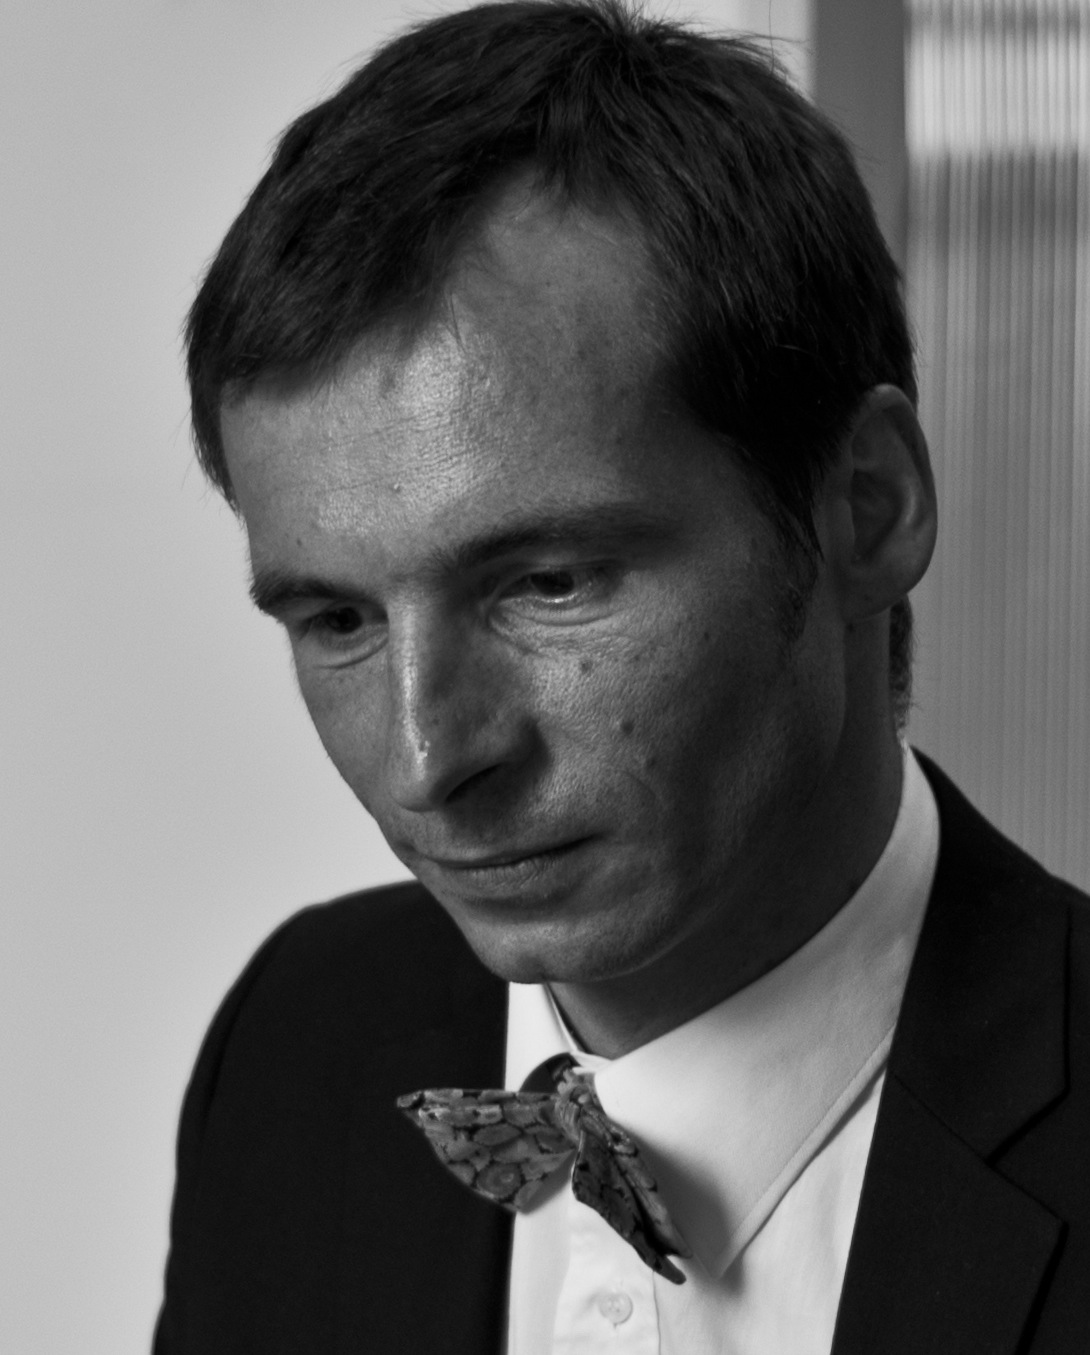
\includegraphics[width=0.28\linewidth]{images/the-opponent.jpg} \hspace{1cm}
			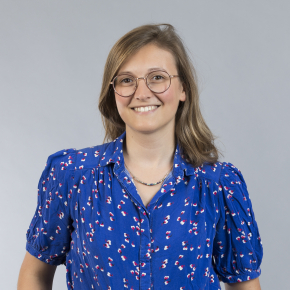
\includegraphics[width=0.35\linewidth]{images/GenevieveRobin_LD_.jpg}
		\end{center}
		\hspace{2cm}C. Ambroise \hspace{3cm}  G. Robin
		\begin{center}
			
\includegraphics[width=0.2\linewidth]{images/UPsaclay.png} 
			
\includegraphics[width=0.1\linewidth]{images/2048px-Centre_national_de_la_recherche_scientifique.svg.png}\hspace{0.1cm}
			
\includegraphics[width=0.12\linewidth]{images/new_logo_univ.png}\hspace{0.15cm}
			
\includegraphics[width=0.08\linewidth]{images/lamme.png}\hspace{0.1cm}
			
\includegraphics[width=0.2\linewidth]{images/Logo-INRAE_Transparent.svg.png}\hspace{0.15cm}
		\end{center}
	\end{frame}
	%====================================================================
	\section{Introduction}
	\subsection{Biological context}
	%====================================================================
	\begin{frame}{Climate change, trees and epigenetics (1)}
		\only<1-2>{
			\centering
			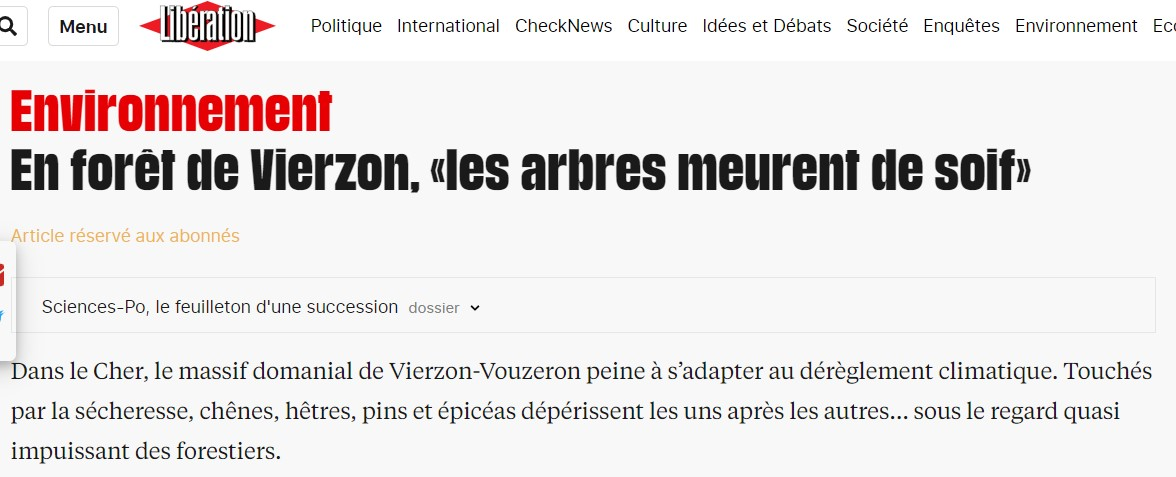
\includegraphics[height=3.5cm]{images/Liberation-environement-vierzon.jpg}	
		}
		\only<3>{
			\centering
			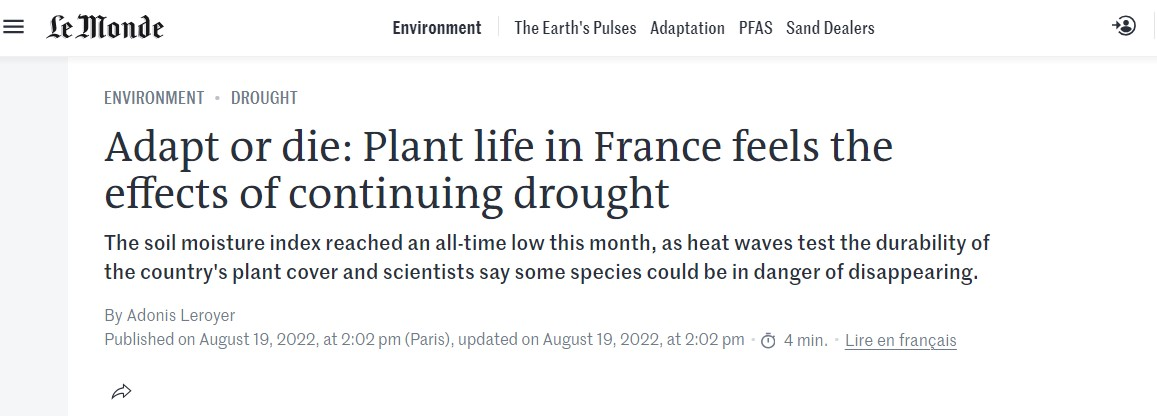
\includegraphics[height=3.5cm]{images/le-monde-environment-plant.jpg}	
		}
		\onslide<1->{
			\begin{block}{Forest \emphase{die-off}}
				\begin{itemize}
					\item Due to drought and heatwave. 
					\item \emphase{Need} to understand the impacts of climate change on forests. 
					\item Key issue: \emphase{Trees' adaptability}.
				\end{itemize}
		\end{block} }
	\end{frame}
	
	\begin{frame}{Climate change, trees and epigenetics (2)}
		\begin{block}{Tree's adaptability \emphase{study}}
			\begin{itemize}
				\item Genetics: DNA sequence and \emphase{genetic evolution}. 
				\item Epigenetics: \emphase{phenotypic plasticity} and environment.
			\end{itemize}
		\end{block}
		
		\begin{block}{\emphase{Example}: Epigenetics and priming in plants}
			
			\centering{
				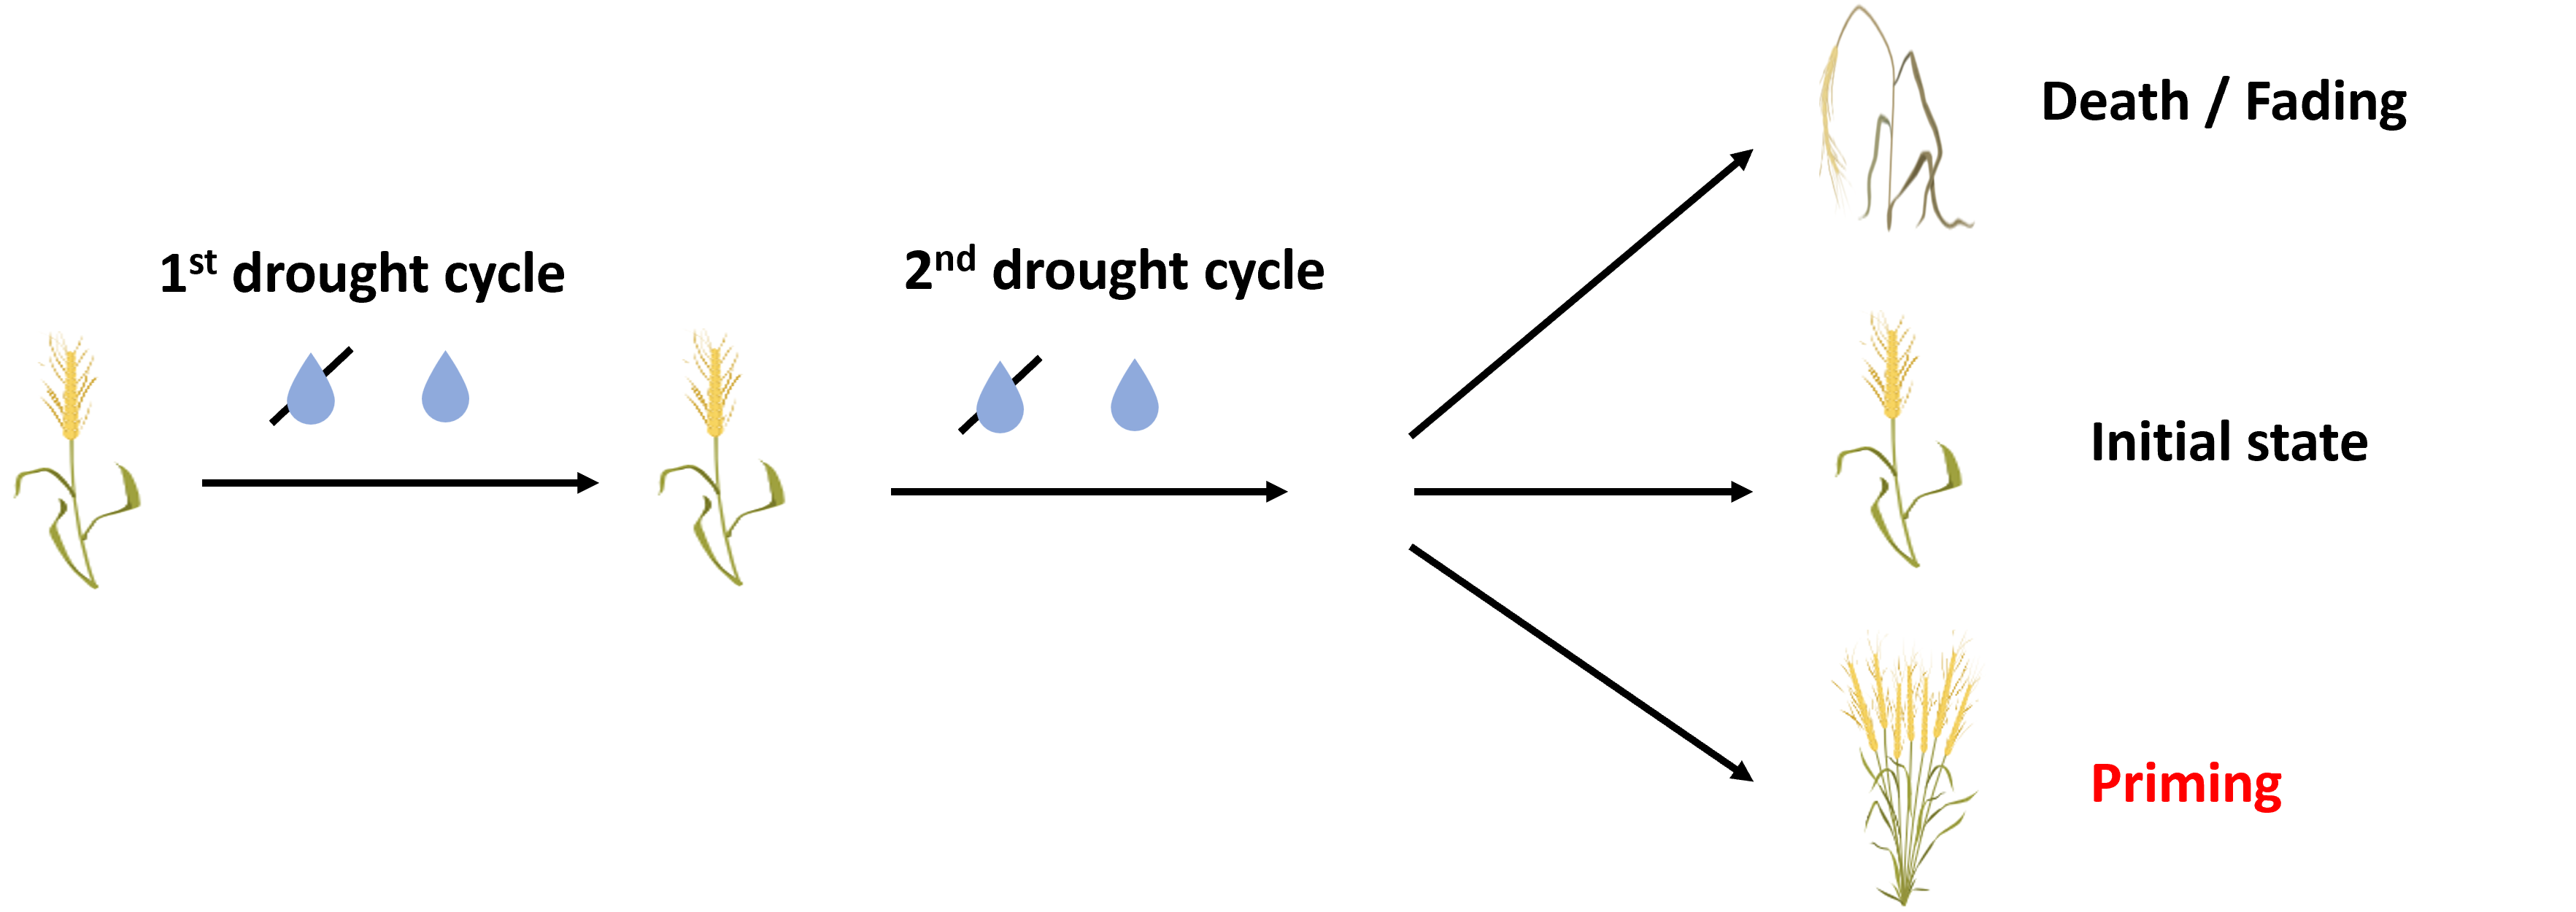
\includegraphics[height=3.5cm]{images/priming.png}}
		\end{block}
	\end{frame}
	
	\begin{frame}{What about \emphase{trees}?}
		
		\begin{columns}
			\begin{column}{2.5cm}
				
\includegraphics[width=2.5cm]{images/epitree.png}
			\end{column}
			\begin{column}{9.5cm}
				
				\begin{block}{EPITREE project}
					Evolutionary and functional impact of epigenetic variation in forest trees.
					%	\begin{itemize}
						%\item Evolutionary and functional impact of \emphase{epigenetic} variation in \emphase{forest trees.}
						%\item Model trees: Poplar and Oak
						%\item Cross-disciplinary teams
						%	\end{itemize}
				\end{block}
				
				\begin{block}{\emphase{Data}}
					Various \emphase{omics} data produced (transcriptomic, DNA methylation, SNPs) and \emphase{phenotypes} data. 
				\end{block}
				
				\begin{block}{\emphase{Example}}
					\centering
					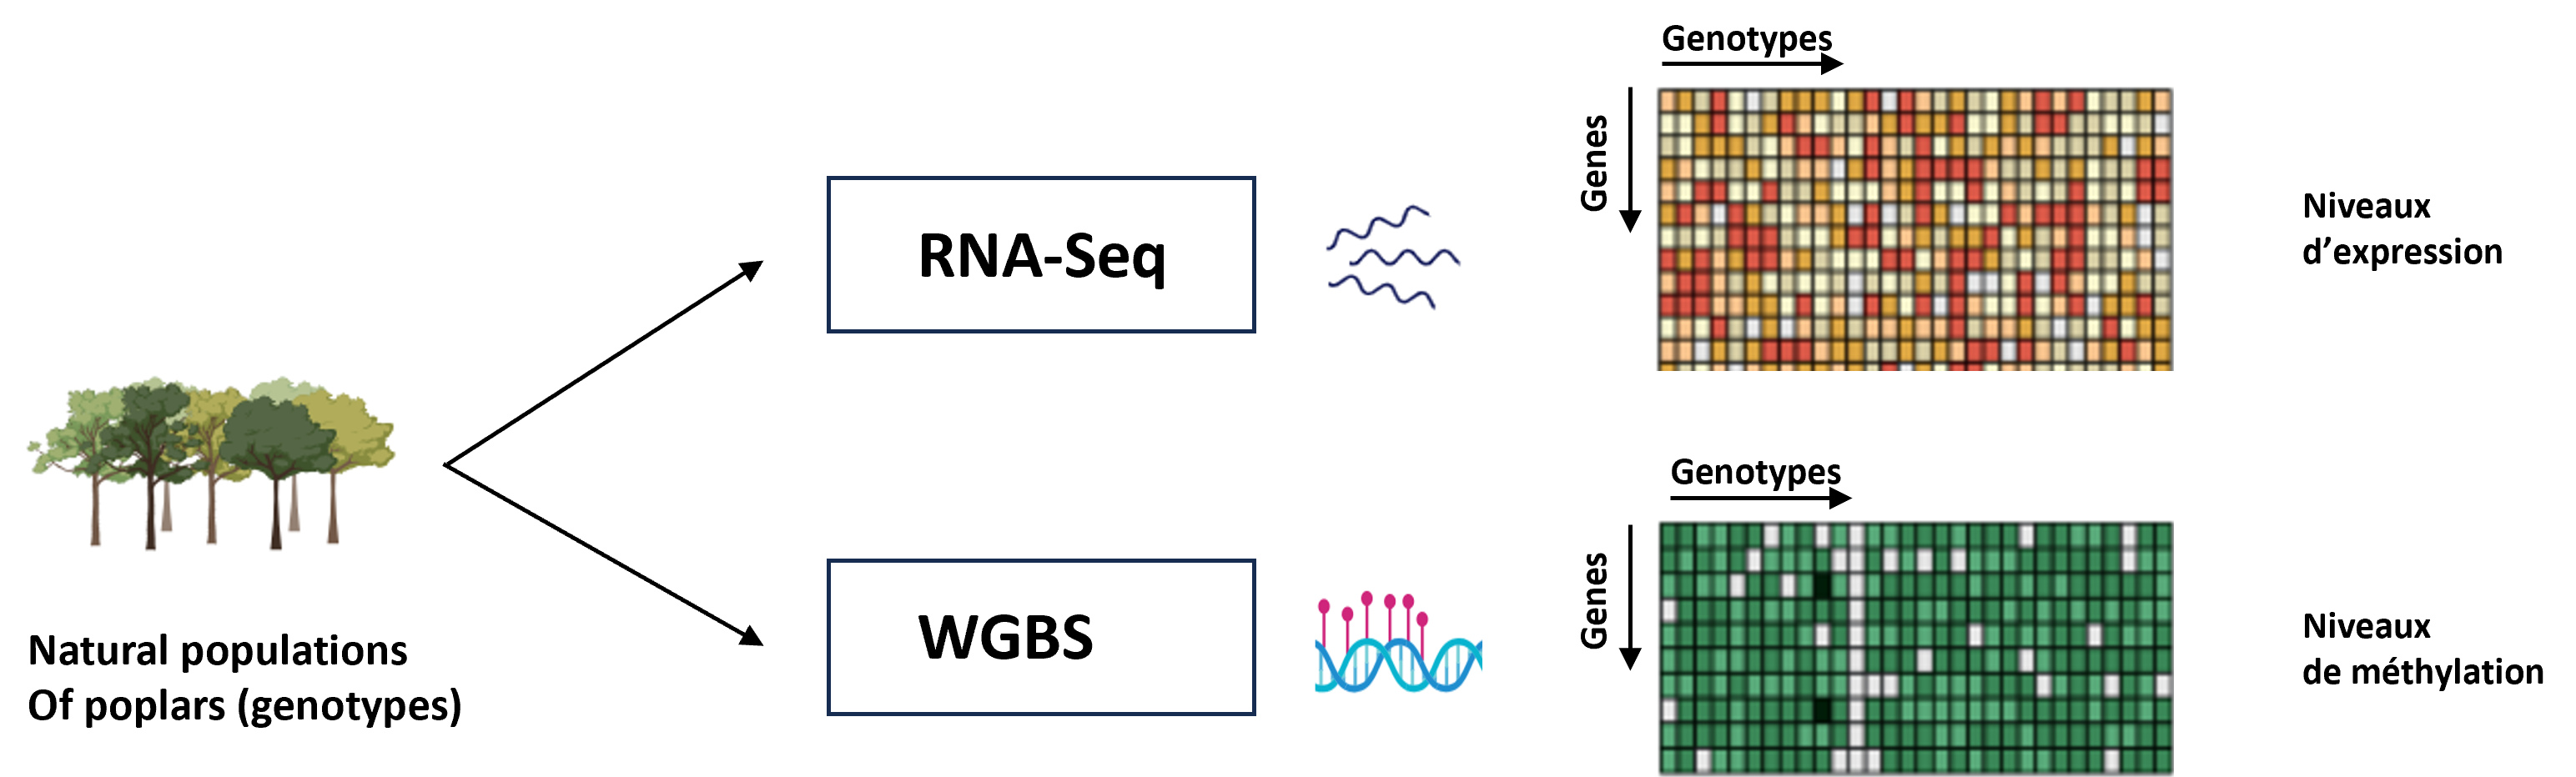
\includegraphics[width=\textwidth]{images/data-measures-methylation-transcriptome.png}
				\end{block}

			\end{column}
		\end{columns}
		%the project
	\end{frame}
	
		\subsection{Network inference}
		\begin{frame}{\emphase{Interactions} in multi-omics data}
			\begin{block}{\emphase{Genotype-Genotype} networks}
				\begin{itemize}
					%\item Interactions between different genotypes within populations 
					\item Co-regulation patterns and  identification of strongly associated genotypes across omics.
				\end{itemize}
			\end{block}
			
			\begin{columns}
				\begin{column}{6cm}
					\begin{block}{\emphase{Example}: One-level network on Transcriptomic and Methylation genotypes}
						\begin{figure}
							\centering
							\resizebox{!}{3.5cm}{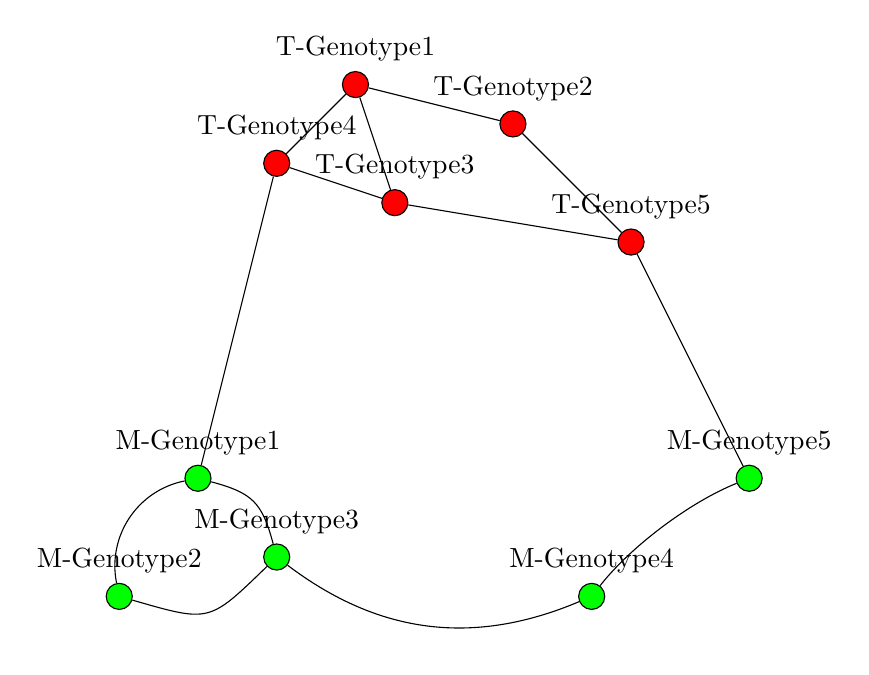
\begin{tikzpicture}[scale=1] % Adjust the scale factor for more space
									% Nodes with labels
									\node [style=node A, label={M-Genotype1}] (0) at (-11, 2) {};
									\node [style=node A, label={M-Genotype2}] (1) at (-12, 0.5) {};
									\node [style=node A, label={M-Genotype3}] (2) at (-10, 1) {};
									
									%\node [style=node A, label={M-Genotype4}] (3) at (-6, 0.5) {};
									\node [style=node B, label={M-Genotype4}] (4) at (-6, 0.5) {};
									\node [style=node B, label={M-Genotype5}] (5) at (-4, 2) {};
									\node [style=node C, label={T-Genotype1}] (6) at (-9, 7) {};
									\node [style=node C, label={T-Genotype2}] (7) at (-7, 6.5) {};
									\node [style=node C, label={T-Genotype3}] (8) at (-8.5, 5.5) {};
									\node [style=node C, label={T-Genotype4}] (9) at (-10, 6) {};
									\node [style=node C, label={T-Genotype5}] (10) at (-5.5, 5) {};
									
									% Edges
									\draw [bend left=45] (1) to (0);
									\draw [bend left, looseness=1.25] (0) to (2);
									\draw [bend right, looseness=1.50] (1) to (2);
									\draw [bend left=15, looseness=0.75] (4) to (5);
									\draw (6) to (7);
									\draw (7) to (10);
									\draw (9) to (8);
									\draw (8) to (10);
									\draw (6) to (9);
									\draw (6) to (8);
									\draw (0) to (9);
									\draw (10) to (5);
									\draw [bend right] (2) to (4);
								\end{tikzpicture}
							}
							%\caption{Your TikZ Diagram Caption}
							%\label{fig:your-diagram}
						\end{figure}
					\end{block}
				\end{column}
				\begin{column}{3cm}
					%		\onslide<3->
					
					\begin{block}{\emphase{Constraints} on building the networks}
						\begin{itemize}
							\item \emphase{Sparsity}
							%				\onslide<4->
							\item \emphase{Clustering structure} 
						\end{itemize}
					\end{block}
				\end{column}
			\end{columns}
			
		\end{frame}
		
		\begin{frame}{\emphase{Two-level} networks}
			
			\begin{block}{\citet{Cheng2017}}
				\begin{itemize}
					\item One level describes networks for variables.
					\onslide<3->{
						\item The other level describes networks for \emphase{known groups}}.
				\end{itemize}
			\end{block}
			\only<2>{
				\centering
				\resizebox{!}{4.5cm}{
					
					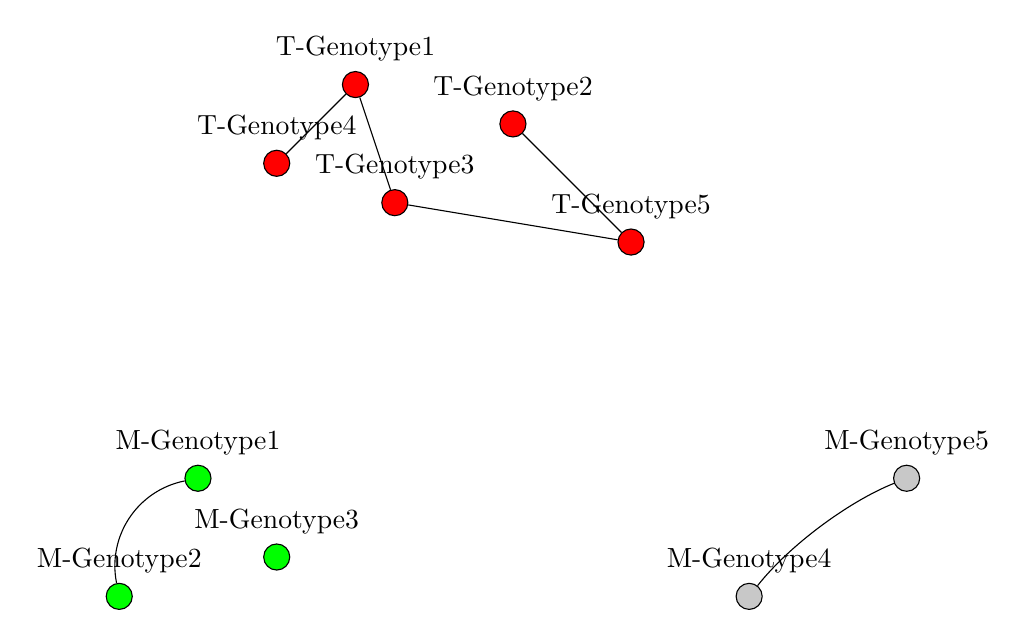
\begin{tikzpicture}[scale=1]
						% Nodes with labels
						\node [style=node A, label={M-Genotype1}] (0) at (-11, 2) {};
						\node [style=node A, label={M-Genotype2}] (1) at (-12, 0.5) {};
						\node [style=node A, label={M-Genotype3}] (2) at (-10, 1) {};
						
						\node [style=node O, label={M-Genotype4}] (4) at (-4, 0.5) {};
						\node [style=node O, label={M-Genotype5}] (5) at (-2, 2) {};
						
						\node [style=node C, label={T-Genotype1}] (6) at (-9, 7) {};
						\node [style=node C, label={T-Genotype2}] (7) at (-7, 6.5) {};
						\node [style=node C, label={T-Genotype3}] (8) at (-8.5, 5.5) {};
						\node [style=node C, label={T-Genotype4}] (9) at (-10, 6) {};
						\node [style=node C, label={T-Genotype5}] (10) at (-5.5, 5) {};
						
						% Edges
						\draw [bend left=45] (1) to (0);
						%\draw [bend left, looseness=1.25] (0) to (2);
						%\draw [bend right, looseness=1.50] (1) to (2);
						\draw [bend left=15, looseness=0.75] (4) to (5);
						%\draw (6) to (7);
						\draw (7) to (10);
						%\draw (9) to (8);
						\draw (8) to (10);
						\draw (6) to (9);
						\draw (6) to (8);

					\end{tikzpicture}
				}
			}
			
			
			\only<3>{

				\centering
				\resizebox{!}{4.5cm}{
					
					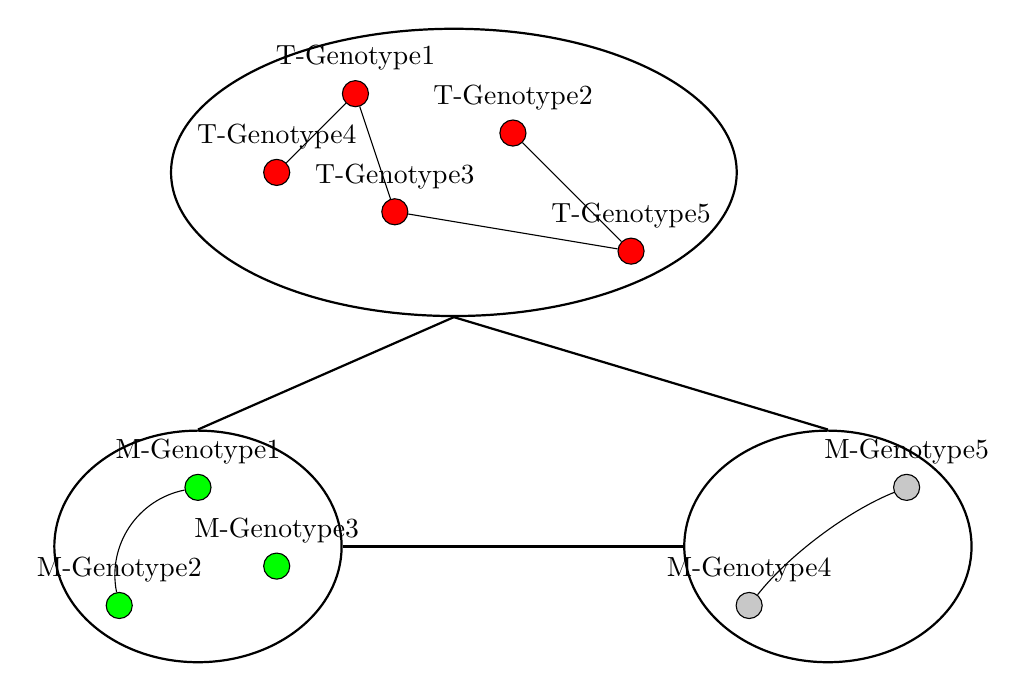
\begin{tikzpicture}[scale=1]
						% Nodes with labels
						\node [style=node A, label={M-Genotype1}] (0) at (-11, 2) {};
						\node [style=node A, label={M-Genotype2}] (1) at (-12, 0.5) {};
						\node [style=node A, label={M-Genotype3}] (2) at (-10, 1) {};
						
						\node [style=node O, label={M-Genotype4}] (4) at (-4, 0.5) {};
						\node [style=node O, label={M-Genotype5}] (5) at (-2, 2) {};
						
						\node [style=node C, label={T-Genotype1}] (6) at (-9, 7) {};
						\node [style=node C, label={T-Genotype2}] (7) at (-7, 6.5) {};
						\node [style=node C, label={T-Genotype3}] (8) at (-8.5, 5.5) {};
						\node [style=node C, label={T-Genotype4}] (9) at (-10, 6) {};
						\node [style=node C, label={T-Genotype5}] (10) at (-5.5, 5) {};
						
						% Edges
						\draw [bend left=45] (1) to (0);
						%\draw [bend left, looseness=1.25] (0) to (2);
						%\draw [bend right, looseness=1.50] (1) to (2);
						\draw [bend left=15, looseness=0.75] (4) to (5);
						%\draw (6) to (7);
						\draw (7) to (10);
						%\draw (9) to (8);
						\draw (8) to (10);
						\draw (6) to (9);
						\draw (6) to (8);
						%\draw (0) to (9);
						%\draw (10) to (5);
						%\draw [bend right] (2) to (4);
						
						
						\begin{scope}[on background layer]
							\node [ellipseNode, fit=(4)(5)] (ellipseB) {};
						\end{scope}
						
						% Group nodes 0, 1, and 2 in an ellipse
						\begin{scope}[on background layer]
							\node [ellipseNode, fit=(0)(1)(2)] (ellipseA) {};
						\end{scope}
						
						% Group nodes 6, 7, 8, 9, and 10 in an ellipse
						\begin{scope}[on background layer]
							\node [ellipseNode, fit=(6)(7)(8)(9)(10)] (ellipseC) {};
						\end{scope}
						
						Draw edges between ellipses
						\draw [black, thick, -] (ellipseA.east) -- (ellipseB.west) node[midway, right, black] {};
						\draw [black, thick, -] (ellipseB.north) -- (ellipseC.south) node[midway, above, black] {};
						\draw [black, thick, -] (ellipseA.north) -- (ellipseC.south) node[midway, below, black] {};
					\end{tikzpicture}
				}
			}
			
				\onslide<4>{
					\begin{block}{Drawbacks}
						\begin{itemize}
							\item Known groups
							\item Only two levels of granularity
						\end{itemize}
					\end{block}
				}
				
				%}
			
		\end{frame}
		
		\begin{frame}{Multilevel/Multiscale networks}
			
			
			\begin{block}{\citet{sanou2023}}
				\begin{columns}
					\begin{column}{0.5\textwidth} % Left column
						\resizebox{!}{4.5cm}{
							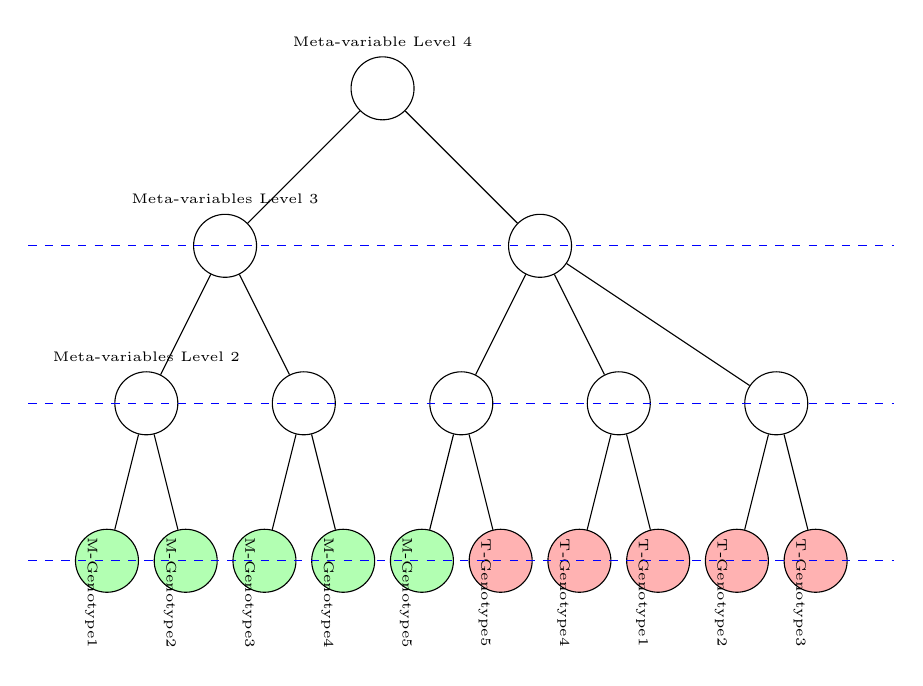
\begin{tikzpicture}[level distance=1.5cm, font=\tiny]
								% Create leaf nodes with rotated labels
								\node[greenLeaf, label={[rotate=-90]below:M-Genotype1}] (A) at (1, 0) {};
								\node[greenLeaf, label={[rotate=-90]below:M-Genotype2}] (B) at (2, 0) {};
								\node[greenLeaf, label={[rotate=-90]below:M-Genotype3}] (C) at (3, 0) {};
								\node[greenLeaf, label={[rotate=-90]below:M-Genotype4}] (D) at (4, 0) {};
								\node[greenLeaf, label={[rotate=-90]below:M-Genotype5}] (E) at (5, 0) {};
								\node[redLeaf, label={[rotate=-90]below:T-Genotype5}] (F) at (6, 0) {};
								\node[redLeaf, label={[rotate=-90]below:T-Genotype4}] (G) at (7, 0) {};
								\node[redLeaf, label={[rotate=-90]below:T-Genotype1}] (H) at (8, 0) {};
								\node[redLeaf, label={[rotate=-90]below:T-Genotype2}] (I) at (9, 0) {};
								\node[redLeaf, label={[rotate=-90]below:T-Genotype3}] (J) at (10, 0) {};
								
								% Create intermediate nodes and connect them
								\node[dendroNode, label={Meta-variables Level 2}] (AB) at (1.5, 2) {};
								\node[dendroNode] (CD) at (3.5, 2) {};
								\node[dendroNode] (EF) at (5.5, 2) {};
								\node[dendroNode] (GH) at (7.5, 2) {};
								\node[dendroNode] (IJ) at (9.5, 2) {};
								
								\node[dendroNode, label={Meta-variables Level 3}] (ABCD) at (2.5, 4) {};
								\node[dendroNode] (EFGH) at (6.5, 4) {};
								
								\node[dendroNode, label={Meta-variable Level 4}] (ABCDEFGH) at (4.5, 6) {};
								
								% Connect the nodes
								\draw (A) -- (AB);
								\draw (B) -- (AB);
								\draw (C) -- (CD);
								\draw (D) -- (CD);
								\draw (E) -- (EF);
								\draw (F) -- (EF);
								\draw (G) -- (GH);
								\draw (H) -- (GH);
								\draw (I) -- (IJ);
								\draw (J) -- (IJ);
								
								\draw (AB) -- (ABCD);
								\draw (CD) -- (ABCD);
								\draw (EF) -- (EFGH);
								\draw (GH) -- (EFGH);
								\draw (IJ) -- (EFGH);
								
								\draw (ABCD) -- (ABCDEFGH);
								\draw (EFGH) -- (ABCDEFGH);
								
								% Draw dotted horizontal blue lines at each level
								\foreach \y in {0, 2, 4} {
									\draw [blue, dashed] (0, \y) -- (11, \y);
								}
							\end{tikzpicture}
						}		
						%\caption{Hierarchical Clustering Tree}
						\onslide<2>{\textcolor{Framaprune}{Challenge}: simultaneous clustering and network inference} 
					\end{column}
					\begin{column}{0.5\textwidth} % Right column
						\begin{minipage}[b]{\textwidth}
							\centering
							\resizebox{1cm}{!}{
								\begin{tikzpicture}[scale=1] % Adjust the scale factor for more space
									% Nodes with labels
									\node [dendroNode] (4) at (-6, 0.5) {};
									\node [dendroNode] (5) at (-4, 2) {};
									% Edges
									\draw [bend left=15, looseness=0.75] (4) to (5);
								\end{tikzpicture}
							}
							\captionof{figure}{Level 3: compressed view}
						\end{minipage}
						\hfill
						\begin{minipage}[b]{\textwidth}
							\centering
							\resizebox{1.5cm}{!}{
								\begin{tikzpicture}[scale=1] % Adjust the scale factor for more space
									% Nodes with labels
									\node [dendroNode] (4) at (-6, 0.5) {};
									\node [dendroNode] (5) at (-4, 2) {};
									\node [dendroNode] (7) at (-7, 6.5) {};
									\node [dendroNode] (8) at (-8.5, 5.5) {};
									\node [dendroNode] (10) at (-5.5, 5) {};
									
									% Edges
									\draw [bend left=15, looseness=0.75] (4) to (5);
									\draw (7) to (10);
									\draw (8) to (10);
									\draw (10) to (5);
								\end{tikzpicture}
							}
							\captionof{figure}{Level 2: compressed view}
						\end{minipage}
						\vspace{1em}
						\begin{minipage}[t]{\textwidth}
							\centering
							\resizebox{!}{2cm}{
								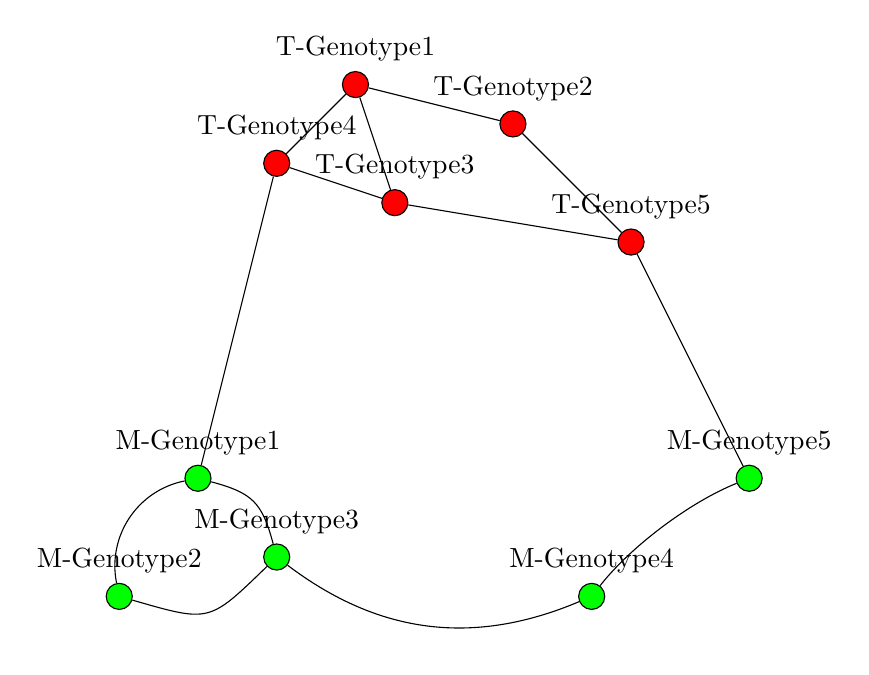
\begin{tikzpicture}[scale=1] % Adjust the scale factor for more space
									% Nodes with labels
									\node [style=node A, label={M-Genotype1}] (0) at (-11, 2) {};
									\node [style=node A, label={M-Genotype2}] (1) at (-12, 0.5) {};
									\node [style=node A, label={M-Genotype3}] (2) at (-10, 1) {};
									
									%\node [style=node A, label={M-Genotype4}] (3) at (-6, 0.5) {};
									\node [style=node B, label={M-Genotype4}] (4) at (-6, 0.5) {};
									\node [style=node B, label={M-Genotype5}] (5) at (-4, 2) {};
									\node [style=node C, label={T-Genotype1}] (6) at (-9, 7) {};
									\node [style=node C, label={T-Genotype2}] (7) at (-7, 6.5) {};
									\node [style=node C, label={T-Genotype3}] (8) at (-8.5, 5.5) {};
									\node [style=node C, label={T-Genotype4}] (9) at (-10, 6) {};
									\node [style=node C, label={T-Genotype5}] (10) at (-5.5, 5) {};
									
									% Edges
									\draw [bend left=45] (1) to (0);
									\draw [bend left, looseness=1.25] (0) to (2);
									\draw [bend right, looseness=1.50] (1) to (2);
									\draw [bend left=15, looseness=0.75] (4) to (5);
									\draw (6) to (7);
									\draw (7) to (10);
									\draw (9) to (8);
									\draw (8) to (10);
									\draw (6) to (9);
									\draw (6) to (8);
									\draw (0) to (9);
									\draw (10) to (5);
									\draw [bend right] (2) to (4);
								\end{tikzpicture}
							}
							\captionof{figure}{Level 1}
						\end{minipage}
					\end{column}
				\end{columns}
				
				
		\end{block}\end{frame}
		
				
		\section{Mathematical framework}
		%====================================================================
		
		
		
		\begin{frame}{}
			\begin{center}
				\Huge{\prune{Mathematical framework}}
			\end{center}
			\normalsize
			\begin{center}
				\begin{description}
					\item[i] {Graphical Models}
					\item[ii]  Convex clustering 
					%\item[iii]  Non-smooth optimization
				\end{description}
			\end{center}
			
		\end{frame}
		
		\subsection{Undirected Graphical Models}
		%==================================================================
		\begin{frame}{Undirected \emphase{Graphical models}}
			\begin{block}{}
				\begin{itemize}
					%\item Marriage between probability theory and graph theory.
					\item Popular computational analysis tool for \emphase{biological} data.
					%\item Conceptual architecture where biological and mathematical objects can be expressed with a common formalism.
					\onslide<3->{\item Describe \emphase{statistical dependencies} between variables.}
				\end{itemize}
			\end{block}
			\bigskip
			\begin{columns}
				
				\begin{column}{0.4\linewidth}\hspace{0.5cm}
					
					
					
					\only<4>{
						\begin{block}{Example: spurrious correlation}
							\begin{figure}
								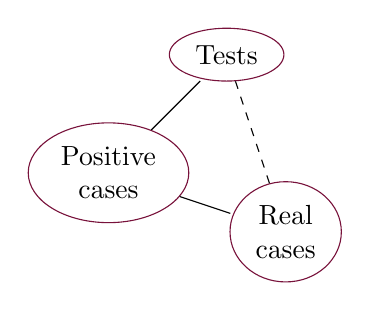
\begin{tikzpicture}
									\tikzstyle{every edge}=[-,>=stealth',shorten >=1pt,auto,thin,draw]
									\node[draw = Framaprune, ellipse, align=center] (X1) at (0*\edgeunit, 0*\edgeunit) {Positive\\ cases};
									\node[draw = Framaprune, ellipse, align=center] (X2) at (1.5*\edgeunit, -0.5*\edgeunit) {Real\\ cases};
									\node[draw = Framaprune, ellipse, align=center] (X3) at (1*\edgeunit, 1*\edgeunit) {Tests};
									\path (X1) edge [] (X2)
									(X1) edge [] (X3);
									\draw [dashed] (X2) -- (X3) node[sloped, above] {};
								\end{tikzpicture}
							\end{figure}
						\end{block}
					}
					
					\onslide<2-3>{\begin{figure}
							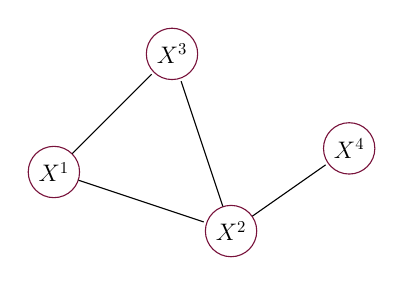
\begin{tikzpicture}	
								\tikzstyle{every edge}=[-,>=stealth',shorten >=1pt,auto,thin,draw]
								\node[observed] (X1) at (0*\edgeunit, 0*\edgeunit) {$X^1$};
								\node[observed] (X2) at (1.5*\edgeunit, -0.5*\edgeunit) {$X^2$};
								\node[observed] (X3) at (1*\edgeunit, 1*\edgeunit) {$X^3$};
								\node[observed] (X4) at (2.5*\edgeunit, 0.2*\edgeunit) {$X^4$};
								\path (X1) edge [] (X2)
								(X1) edge [] (X3)
								(X2) edge [] (X3)
								(X2) edge [] (X4);
							\end{tikzpicture}
							\caption{\emphase{Undirected graph.}}
					\end{figure}}
				\end{column}
				\only<3>{
					\begin{column}{0.5\linewidth}
						\begin{itemize}
							\item Connected: \emphase{conditional dependence} \\\bigskip
							\emphase{Markov property}: $X^4$ is independent from  $(X^1, X^3)$ conditionally to  $X^2$ \vspace{0.2cm}
							%\item Probabilistic background\\$p(a,b\mid c) = p(a\mid c)\, p(b \mid c)$.
						\end{itemize}
				\end{column}}
			\end{columns}
		\end{frame}
		


\begin{frame}{Undirected Graphical Models}
	%Key idea: write the joint distribution as a product of clique wise potential functions.
	
	%Pair $(G,\mathbb P)$ where $G$ is a graph with undirected edges and $\mathbb P$ is a distribution that factorizes with respect to $G.$ 
	Pair $(G,\mathbb P)$ where $\mathbb P$ is a distribution that \emphase{factorizes} with respect to the graph $G.$ \\
	Let $X = (X^1, \dots,  X^p)$ be a random vector taking values in $\chi.$ 
	\vspace{0.5cm}
	\begin{block}{Factorization}
		%and $\mathcal C$ the set of maximal cliques of the graph $G$.
		%$$\mathbb P (X) = \frac{1}{Z} \prod_{C \in \textcolor{Framaprune}{\mathcal{C}}} \textcolor{Framaprune}{\phi_C}(\textcolor{Framaprune}{X^C}).$$
		\begin{equation*}
			\mathbb P (X) = \tikzmarknode[]{identity}{\frac{1}{Z}} \tikzmarknode[]{G}{\prod_{C \in \mathcal{C}}}\,\,\, 
			\tikzmarknode[]{L}{\phi_C} ( \tikzmarknode[]{C}{X^C})
		\end{equation*}
		\begin{tikzpicture}[overlay, remember picture,node distance =1.5cm]
			
			\node (identitydescr) [below left=of identity, yshift=0.7cm ]{\emphase{Partition} function};
			\draw[,->,thick] (identitydescr) to [in=-90,out=90] (identity);
			
			\node[yshift=0.8cm] (Gdescr) [below =of G]{Product over \emphase{cliques}};
			
			\draw[,->,thick] (Gdescr) to [in=-90,out=90] (G);
			
			\node[] (Ldescr) [above right =of L, yshift=-2]{\emphase{Potential} function};
			\draw[,->,thick] (Ldescr) to [in=45,out=-90] (L.north);
			
			\node[] (Cdescr) [below right =of C, xshift=-0.2]{Variables in clique $C$};
			\draw[,->,thick] (Cdescr) to [in=-90,out=90] (C.south);
		\end{tikzpicture}
		
	\end{block}
	
	%Exponential formulation
	%\begin{equation*}
	%	\mathbb P(X) = \exp \left(  \sum_{C \in \mathcal{C}} \log \left(\phi_C(X^C)\right) \right).
	%\end{equation*}
	%
	%Pairwise Markov Random Fields
	%\begin{equation*}
	%	\mathbb P(X) = \exp \left ( \sum_{i=1}^p \theta_i f_i(X^i) + \sum_{i < j} \theta_{ij} f_{ij} (X^i, X^j) \right )
	%\end{equation*}
	\vspace{1cm}
	\textcolor{Framaprune}{Some distributions for $\phi_C$}
	\begin{itemize}
		\item Ising model: $\chi = \{ 0,1\}$ 
		\item Potts model: $\chi = \{1, \dots, m\}$ 
		\item Gaussian model: $\chi = \mathbb{R}$ 
	\end{itemize}
	
	%				\tikzstyle{every edge}=[-,>=stealth',shorten >=1pt,auto,thin,draw]
	%\node[observed] (X1) at (0*\edgeunit, 0*\edgeunit) {$X^1$};
	%\node[observed] (X2) at (1.5*\edgeunit, -0.5*\edgeunit) {$X^2$};
	%\node[observed] (X3) at (1*\edgeunit, 1*\edgeunit) {$X^3$};
	%\node[observed] (X4) at (2.5*\edgeunit, 0.2*\edgeunit) {$X^4$};
	%\path (X1) edge [] (X2)
	%(X1) edge [] (X3)
	%(X2) edge [] (X3)
	%(X2) edge [] (X4);
\end{frame}

\begin{frame}{Gaussian Graphical Models (GGM)}
	\textcolor{Framaprune}{Gaussian distribution}\\
	Let $\Xbf\sim \mathcal{N}(0_p, \Sigmab)$ with precision matrix $\Omegab=\Sigmab^{-1}.$
	
	\only<1>{
		\begin{equation*}
			\mathbb P_{\mathbf \Omega} (\Xbf) = \frac{\left (\det(\Omegab) \right ) ^{1/2}}{(2 \pi)^{p/2}} \exp \left \{ -\frac{1}{2} \Xbf^\top \Omegab \Xbf \right \}
		\end{equation*}
	}
	
	\onslide<2->{
		\begin{equation*}
			\mathbb P_{\mathbf \Omega}(\Xbf) = \frac{1}{\textcolor{Framaprune}{Z_{\mathbf \Omega}}} \exp \left \{ -\frac{1}{2} \sum_{s,t=1}^p \textcolor{Framaprune}{\Omega_{st}}X^sX^t \right \}
		\end{equation*}
	}
	
	\only<3>{
		\textcolor{Framaprune}{Based on the factorization (Hammersley-Clifford)}
		\vspace{0.3cm}
		\begin{columns}
			\begin{column}{0.4\linewidth}
				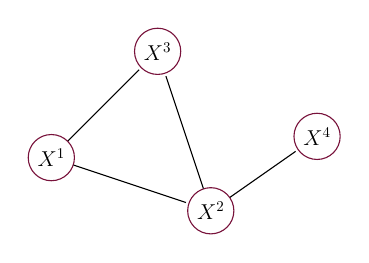
\begin{tikzpicture}[scale=0.9]
					\tikzstyle{every edge}=[-,>=stealth',shorten >=1pt,auto,thin,draw]
					\node[observed] (X1) at (0*\edgeunit, 0*\edgeunit) {$X^1$};
					\node[observed] (X2) at (1.5*\edgeunit, -0.5*\edgeunit) {$X^2$};
					\node[observed] (X3) at (1*\edgeunit, 1*\edgeunit) {$X^3$};
					\node[observed] (X4) at (2.5*\edgeunit, 0.2*\edgeunit) {$X^4$};
					\path (X1) edge [] (X2)
					(X1) edge [] (X3)
					(X2) edge [] (X3)
					(X2) edge [] (X4);
				\end{tikzpicture}
			\end{column}
			\begin{column}{0.1\linewidth}
				\emphase{$\iff$ }
			\end{column}
			\begin{column}{0.4\linewidth}
				$\Omegab=\left(\begin{array}{llll}
					*&*&*&\emphase{0}\\
					*&*&*&*\\
					*&*&*&\emphase{0}\\
					\emphase{0}&*&\emphase{0}&*
				\end{array}\right) $
			\end{column}
		\end{columns}
	}
	%	\begin{itemize}
		%		%\item   We have 
		%		% $$f(\Xbf) \propto \prod_{j,k, {\Omega_{jk}\neq 0}} \exp(-X^{k}\Omega_{jk}X^{j}/2).$$
		%		\item Inferring GGM: learning the structure of $\Omegab.$
		%	\end{itemize}
	
	%\begin{block}{Partial correlation \& precision matrix}
	%	\begin{itemize}
		%		\item  Conditional dependencies encoded in \emphase{partial correlations}
		%		\item $\operatorname{cor}(X^j, X^k | \Xbf^{\setminus (j, k)}) = -\Omega_{jk}/\sqrt{\Omega_{jj}\Omega_{kk}} \quad \forall j \neq k$
		%	\end{itemize}
	%\end{block}
	%Two ways of estimating the structure of $\Omega$
\end{frame}

\begin{frame}{Maximum likelihood estimator}
	
	\begin{itemize}
		\item Log-likelihood
		$$\log \mathcal{L}(\Xbf, \Omegab) = \sum_{i=1}^n \log \mathbb P(X_i; \Omegab) \propto \log \det (\Omegab) - \operatorname{tr}(\Xbf ^\top \Xbf \Omegab)$$
		\item Solution 
		$$\widehat \Omegab_{MLE} = \argmax_{\mathbf \Omega} \log \mathcal{L}(\Xbf, \Omegab) = \mathbf S^{-1}$$ %with $\mathbf S$ non-singular.
		%	The solution to the likelihood maximization problem is unique and given by  
		%	$\widehat \Omegab_{MLE} = \mathbf S^{-1}$
		%	whenever $\mathbf S$ is non singular, with $\mathbf S = \frac{1}{n}\mathbf X^\top \mathbf X.$
	\end{itemize}
	
	\begin{block}{Drawbacks}
		\begin{itemize}
			\item Singularity of the covariance matrix in high dimension
			\item Complete graphs
			% one drawback related to pseudo likelihood advantage \item %
		\end{itemize}
	\end{block}
\end{frame}

\begin{frame}{Maximum pseudo-likelihood estimator}
	%Regression based estimation   
	%Let $\Xbf\sim \mathcal{N}(0_p, \Sigmab).$  
	
	\begin{itemize}
		\item Conditional distribution 
		%The conditional distribution of $X^i|\Xbf^{\backslash i}$  is gaussian.
		$$X^i|X^{\backslash i} = X^{\backslash i} \sim \mathcal N \left ( -\Omega_{ii}^{-1} \Omega_{i\backslash i}  X^{\backslash i}, ~~ \Omega_{ii}^{-1} \right).$$
		\item Solving $p$ \emphase{linear regressions}
		%One may use $p$ different \emphase{linear regressions} to learn the structure of $\Omegab.$
		\small $$\boldsymbol X^i = \Xbf^{\setminus i} \boldsymbol \beta^i + \boldsymbol \epsilon, \quad \quad \text{where} \quad \boldsymbol \beta^i = - \boldsymbol \Omega_{i \backslash i}/\Omega_{ii}, \forall i=1, \dots, p$$
		\item A pseudo-likelihood criterion \citep{Ambroise2009}
		%Proceeding so is equivalent to maximizing a pseudo-likelihood criterion \citep{Ambroise2009} with:
		$$\hat{\boldsymbol{\beta}} = \argmax_{\boldsymbol{\beta}} \log \tilde{\mathcal L} (\Xbf, \boldsymbol{\beta}) = \argmax_{\boldsymbol{\beta}} \sum_{i=1}^n \sum_{j=1}^p \mathbb \log P \left (X_j^i | X^{\setminus i}_j; \boldsymbol \beta^i \right)$$
	\end{itemize}
\end{frame}

\begin{frame}{Estimation with sparsity constraint}
	%structural constraints 
	%% lasso 
	%% grouping penalties 
	
	% Challenges 
	% 1 Clustering / regression 
	% grouping regressions 
	%Structural constraints; Lasso penalty: neighborhood selection 
	
	\textcolor{Framaprune}{Neighborhood selection \citep{Meinshausen2006}}
	\begin{itemize}
		\item Solve $p$ independant Lasso regression problems:
		\small $$\hat{\boldsymbol \beta^i}(\lambda) = \argmin_{\boldsymbol \beta^i} \frac{1}{n} || \boldsymbol X^i - \mathbf X^{\setminus i} \boldsymbol \beta^i ||_2^2 + \lambda||\boldsymbol \beta^i||_1, \forall i=1, \dots, p $$
	\end{itemize}
	
	\begin{block}{Drawbacks}
		\begin{itemize}
			\item Limitations of Lasso in the presence of strongly correlated variables 
		\end{itemize}
	\end{block}
	
	\begin{block}{Alternative approaches in single task regression problems}
		\begin{itemize}
			\item In two-step: clustering followed by regression e.g. Cluster representative Lasso \citep{Buhlmann2012}
			% followed by estimation on cluster representative variables e.g. Cluster representative Lasso
			\item In one-step: penalty functions for grouping e.g. Fused-Lasso \citep{Tibshirani2005}
		\end{itemize}
	\end{block}
\end{frame}

\begin{frame}{Challenges in multitask learning}
	%Challenge in defining fusion penalties for Multitask regression problems 
	\textcolor{Framaprune}{Framework}
	\begin{itemize}
		\item $p$ responses variables: $\boldsymbol X^1, \dots, \boldsymbol X^p \in \mathbb R^{n}$ 
		\item $p$ sets of explanatory variables $\Xbf^{\backslash 1}, \dots, \Xbf^{\backslash p} \in \mathbb R^{n, p-1}$ 
		\item $p$ regression vectors $\boldsymbol \beta^1, \dots, \boldsymbol \beta^{p} \in \mathbb R^{p-1}$ giving the neighborhood structure the variables
		\item The pseudo log-likelihood writes:
		$$\frac{1}{2} \sum_{i=1}^p \left
		\lVert \mathbf{X}^i - \mathbf{X}^{\setminus i} \boldsymbol{\beta}^i \right
		\rVert_2 ^2  + \lambda_1 \sum_{i = 1}^p  \left \lVert \boldsymbol{\beta}^i
		\right \rVert_1$$
	\end{itemize}
	
	\textcolor{Framaprune}{Challenge: penalty for grouping over non-fixed set of covariates }
	$$\frac{1}{2} \sum_{i=1}^p \left
	\lVert \mathbf{X}^i - \mathbf{X}^{\setminus i} \boldsymbol{\beta}^i \right
	\rVert_2 ^2  + \lambda_1 \sum_{i = 1}^p  \left \lVert \boldsymbol{\beta}^i
	\right \rVert_1 + \textcolor{Framaprune}{pen(\boldsymbol{\beta}^i, \dots, \boldsymbol{\beta}^p)}$$
\end{frame}



\subsection{Clustering}

%\begin{frame}{Clustering}
% 	% Definition 
% 	%% Kmeans 
% 	%% HAC 
% 	% Illustration of instability in kmeans 
% 	% Illustration of instability in HAC
% 	\begin{itemize}
	% 		\item Fundamental cornerstone of pattern recognition, machine learning and statistics 
	% 		\item Divide datapoints into groups based on common properties.
	% 		\item Tons of clustering algorithms developped.
	% 	\end{itemize}
% 	
% 	\textcolor{Framaprune}{Popular techniques}
% 	\begin{itemize}
	% 		\item $K$-means partitionning (since the 1950s)
	% 		\begin{itemize}
		% 			\item Alternate minimizes the square error criterion $\sum_{i=1}^K \sum_{i\in S_k} d(x_i, \alpha_k)$ 
		% 			\item Weakness: sensitive to initialization and require number of clusters.
		% 		\end{itemize} 
	% 		\item Hierarchical agglomerative clustering (HAC)
	% 		\begin{itemize}
		% 			\item Represent data in the form of a hierarchy 
		% 			\item Drawbacks: instability of clustering partitions and greedy algorithm.
		% 		\end{itemize}
	% 	\end{itemize}
% \end{frame}

\begin{frame}{Convex clustering}
Let $\boldsymbol x_i \in \mathbb R^{p}$ be datapoints and $\boldsymbol \alpha_i \in \mathbb R^{p}$ corresponding centroids with $i=1, \dots, n.$

\emphase{Convex} clustering \citep{pelckmans2005convex, Hocking2011, Lindsten2011} solves:
\begin{equation*}
	\argmin_{\boldsymbol \alpha \in \mathbb R^{n\times p}} \underbrace{\frac{1}{2} \sum_{i=1}^n||x_i - \boldsymbol \alpha_i||_2^2}_{Clustering~loss} + \underbrace{\lambda \sum_{i < j} ||\boldsymbol \alpha_i - \boldsymbol \alpha_j||_q}_{Shrinkage~term}
\end{equation*}
\begin{itemize}
	%\item Convex version of the hierarchical clustering 
	%\item Constrains the rows of a $\alpha \in \mathbb R^{n\times p} $ matrix of centroids to be identical.
	\item Global optimum reached and independent of initialization.
	\item $\lambda$ determines the number of clusters.
	\item Choice of the $q$-norm influences solutions' path.
\end{itemize}
\end{frame}

\begin{frame}{Clustering path}
\begin{figure}
	\centering
	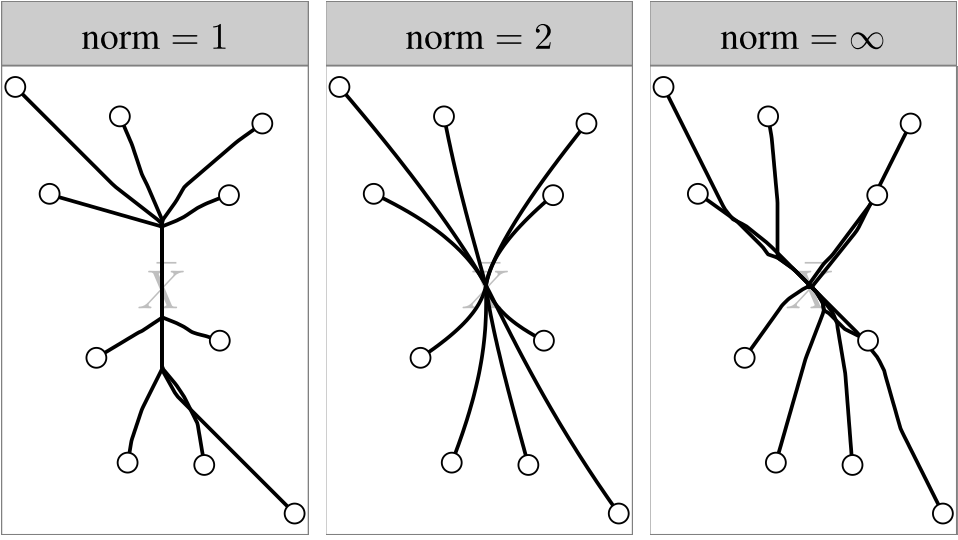
\includegraphics[scale=0.5]{images/clusterpath-Hocking.png}
	\caption{Clustering path for different norms \citep{Hocking2011}}
\end{figure}
\end{frame}


%\begin{frame}{}
%	\only<1>{
%			\begin{tikzpicture}[scale=0.8]
	%			\begin{axis}[
		%				width=\linewidth,
		%				title={KMeans Clustering ($k=2$)},
		%				xmin=0,xmax=10,ymin=0,ymax=10,
		%				xlabel={x},
		%				ylabel={y}
		%				]
		%				%\node[text=blue,font=\sffamily\bfseries,scale=2] at (3,3) {X};
		%				\addplot+[y filter/.expression={y+1},only marks,mark=*,samples=50,domain=1:5] {4*rnd};
		%				%\node[text=red,font=\sffamily\bfseries,scale=2] at (7,7){X};
		%				\addplot+[y filter/.expression={y+5},only marks,mark=*,mark options={fill=lightgray},samples=50,domain=5:9] {4*rnd};
		%			\end{axis}
	%		\end{tikzpicture}
%	}
%	\only<2>{
%			\begin{tikzpicture}[scale=0.8]
	%			\begin{axis}[
		%				width=\linewidth,
		%				title={KMeans Clustering ($k=2$)},
		%				xmin=0,xmax=10,ymin=0,ymax=10,
		%				xlabel={x},
		%				ylabel={y}
		%				]
		%				\node[text=blue,font=\sffamily\bfseries,scale=2] at (3,3) {X};
		%				\addplot+[y filter/.expression={y+1},only marks,mark=*,samples=50,domain=1:5] {4*rnd};
		%				\node[text=red,font=\sffamily\bfseries,scale=2] at (7,7){X};
		%				\addplot+[y filter/.expression={y+5},only marks,mark=*,mark options={fill=red},samples=50,domain=5:9] {4*rnd};
		%			\end{axis}
	%		\end{tikzpicture}
%	}
%\end{frame}

%\begin{frame}{Convex clustering}
%	% Solution path 
%	% Optimization methods 
%	% ? Introduce conesta in the mglasso section 
%\end{frame}

%\begin{frame}{Clustering path}
%	\begin{figure}
%		\centering
%		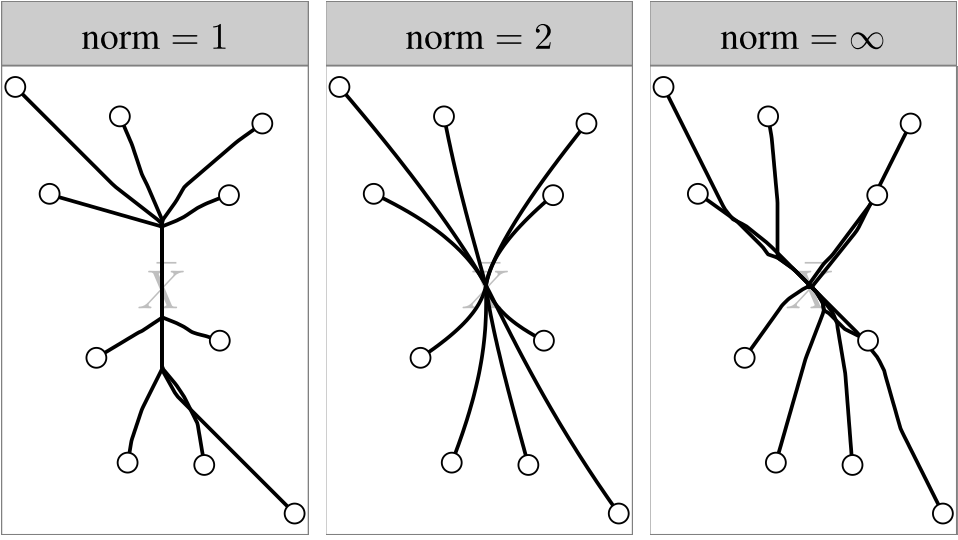
\includegraphics[scale = 0.5]{images/clusterpath-Hocking.png}
%		\caption{Clustering path for different norms \citep{Hocking2011}}
%	\end{figure}
%	
%	 Notion of equality between coefficients centroids
%	 Conditions under which this is a hierarchical tree?
%	 Park paper on aggregation?
%	 Clusters membership
%\end{frame}

% \begin{frame}{Getting back to Gaussian data}
% \begin{center}
	%\begin{tikzpicture}
	%      \tikzstyle{every edge}=[-,>=stealth',shorten >=1pt,auto,thin,draw]
	%		\node (A1) at (0*\edgeunit, 0*\edgeunit) {
		%		\includegraphics[width=3cm]{images/discret.png}};
	%		\node (A2) at (5*\edgeunit, 0*\edgeunit) {
		%		\includegraphics[width=3cm]{images/continu.png}};
	%	 \node (A3) at (2.5*\edgeunit, 1.25*\edgeunit) {\text{Transformations}};
	%	  \node (A4) at (2.5*\edgeunit, 0.15*\edgeunit) {\text{Copulas}};
	%	   
	%		\path (A1) edge [->, bend left] (A2) 
	%		(A1) edge [->] (A2);
	%	
	%		\node (A5) at (2.5*\edgeunit, -1.25*\edgeunit) {\emphase{\text{Latent variables}}};
	%		\path (A1) edge [->, bend right] (A2) ;
	%	%  
	%		\node (A6) at (2.5*\edgeunit, -2.5*\edgeunit) {\text{Modeling counts with Gaussian latent parameters}};
	%		\path (A5) edge [->] (A6) ;
	%\end{tikzpicture}
	% \end{center}
% \end{frame}

%=======================================
%%%%%%%%%%%%%%%%%%%%%%%%%%%%%%%%%%
%%%%%%%%%%%%%%%%%%%%%%%%%%%%%%%%%%

\section{Multiscale Gaussian Graphical Model}
\begin{frame}{}
\begin{center}
	\Huge{\prune{Multiscale Gaussian Graphical Model}}
\end{center}
\begin{center}
	\begin{description}
		\item[i] Model
		\item[ii] Inference
	\end{description}
\end{center}
\end{frame}

%=======================================
\subsection{Model}
\begin{frame}{Intuition}
\centering
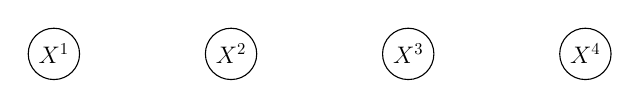
\begin{tikzpicture}	[scale=1]
	\tikzstyle{every edge}=[-,>=stealth,shorten >=1pt,auto,thin,draw]
	\tikzstyle{every node}=[scale=0.6,circle,draw=black,transform shape,fill=white,font=\Large]
	\node (X1) at (0*1.5, 0*1.5) {$X^1$};
	\node[] (X2) at (1.5*1.5, 0*1.5) {$X^2$};
	\node[] (X3) at (3*1.5, 0*1.5) {$X^3$};
	\node[] (X4) at (4.5*1.5, 0*1.5) {$X^4$};
	%(X2) edge [bend right = 25] (X4)
	%(X2) edge [bend left = 35] (X3);
\end{tikzpicture}
\begin{itemize}
	\item Identify the \emphase{neighborhood} of each node \\ $\rightarrow$ via Lasso selection: $\sum_{i = 1}^p  \left \lVert \boldsymbol{\beta}^i
	\right \rVert_1$ 
	\vspace{0.2cm}
	\begin{center}
		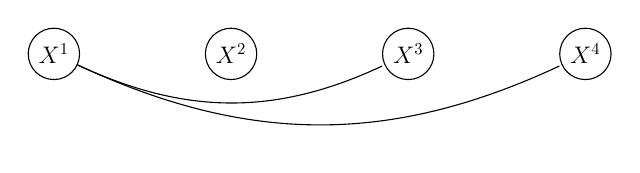
\begin{tikzpicture}	[scale=1]
			\tikzstyle{every edge}=[-,>=stealth,shorten >=1pt,auto,thin,draw]
			\tikzstyle{every node}=[scale=0.6,circle,draw=black,transform shape,fill=white,font=\Large]
			\node (X1) at (0*1.5, 0*1.5) {$X^1$};
			\node[] (X2) at (1.5*1.5, 0*1.5) {$X^2$};
			\node[] (X3) at (3*1.5, 0*1.5) {$X^3$};
			\node[] (X4) at (4.5*1.5, 0*1.5) {$X^4$};
			\path (X1) edge [bend right = 25] (X3)
			(X1) edge [bend right = 25] (X4);
			%(X2) edge [bend right = 25] (X4)
			%(X2) edge [bend left = 35] (X3);
		\end{tikzpicture}
	\end{center}
	\item Group variables with similar neighborhood structure (\emphase{Local constancy}) \\ $\rightarrow $ via group-fused Lasso: $\sum_{i < j} \left \lVert \emphase{
		\boldsymbol{\beta}^i }  - \emphase{\boldsymbol \tau_{ij}} \boldsymbol{\beta}^j \right \rVert_2$ 
	\vspace{0.2cm}
	\begin{center}
		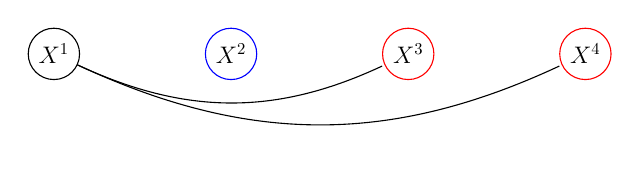
\begin{tikzpicture}	[scale=1]
			\tikzstyle{every edge}=[-,>=stealth,shorten >=1pt,auto,thin,draw]
			\tikzstyle{every node}=[scale=0.6,circle,draw=black,transform shape,fill=white,font=\Large]
			\node (X1) at (0*1.5, 0*1.5) {$X^1$};
			\node[draw=blue] (X2) at (1.5*1.5, 0*1.5) {$X^2$};
			\node[draw=red] (X3) at (3*1.5, 0*1.5) {$X^3$};
			\node[draw=red] (X4) at (4.5*1.5, 0*1.5) {$X^4$};
			\path (X1) edge [bend right = 25] (X3)
			(X1) edge [bend right = 25] (X4);
			%(X2) edge [bend right = 25] (X4)
			%(X2) edge [bend left = 35] (X3);
		\end{tikzpicture}
	\end{center}
	
	%	\caption{Illustration of locality graph in the MGLasso model with $4$
		%		variables. All the nodes are expected to be local neighbors. The
		%		pairwises differences includes all the existing pairs of variables.}
	%	\label{fig-local-cst-mglasso}
	
	%\item Take in account the non fixed set of covariates problem via permutations
	%\begin{figure}[H]
	%	\begin{equation*}
		%		(\boldsymbol \beta^i,  \textcolor{black}{\boldsymbol \tau_{ij}}
		%		\boldsymbol \beta^j)  =
		%		\begin{pmatrix}
			%			\beta_1^i & \beta_2^i & \dots & \tikzmarknode{a}{\beta_j^i} &
			%			\dots \dots & \tikzmarknode{b}{\beta_k^i} & \dots & \beta_p^i\\
			%			\\
			%			\\
			%			\beta_1^j & \beta_2^j & \dots & \tikzmarknode{c}{\beta_k^j} &
			%			\dots \dots & \tikzmarknode{d}{\beta_i^j} & \dots & \beta_p^j
			%		\end{pmatrix}
		%	\end{equation*}
	%	\begin{tikzpicture}[remember picture,overlay]
		%		\draw[black,-latex]([yshift=0.1ex]d.south) to[bend left]node[below]{}
		%		([yshift=0.1ex]c.south);
		%		\draw[black,-latex]([yshift=-.1000ex]c.north) to[bend left]node[below]{}
		%		([yshift=-.1000ex]d.north);
		%	\end{tikzpicture}
	%	%\caption{Illustration of the permutation between regression coefficients in the MGLASSO model.}
	%	\label{fig:permute-beta}
	%\end{figure}
\end{itemize}
\end{frame}


\begin{frame}{Formulation}
The Multiscale Graphical LASSO (MGLASSO, \cite{sanou2023}) problem minimizes the following pseudo-likelihood criterion:
\only<1>{
	\small $$
	\mathcal J_{\lambda_1,
		\lambda_2}(\boldsymbol{\beta}; \mathbf{X} ) = \frac{1}{2} 
	\underbrace{\sum_{i=1}^p \left
		\lVert \mathbf{X}^i - \mathbf{X}^{\setminus i} \boldsymbol{\beta}^i \right
		\rVert_2 ^2  + \lambda_1 \sum_{i = 1}^p  \left \lVert \boldsymbol{\beta}^i
		\right \rVert_1}_{Neighborhood~selection} + \underbrace{\lambda_2 \sum_{i < j} \left \lVert \boldsymbol{\beta}^i -
		\boldsymbol \tau_{ij}\boldsymbol{\beta}^j \right \rVert_2}_{convex~clustering},
	\label{eq:cost-fct}
	$$
	with 
	$\left
	\lVert \boldsymbol{\beta}^i - \boldsymbol \tau_{ij}\boldsymbol{\beta}^j \right
	\rVert_2 = \sqrt{\sum_{k \in \{1, \dots,p \} \backslash \{i,j\}} (\beta^i_k -
		\beta^j_k)^2 + (\beta^i_j - \beta^j_i)^2 }.$
}

\onslide<2>{
	$$\mathcal J_{\lambda_1,
		\lambda_2}(\boldsymbol{\beta}; \mathbf{X} ) = \frac{1}{2} 
	\underbrace{\sum_{i=1}^p \left
		\lVert \mathbf{X}^i - \mathbf{X}^{\setminus i} \boldsymbol{\beta}^i \right
		\rVert_2 ^2}_{Smooth}  + \underbrace{\textcolor{Framaprune}{\lambda_1 \sum_{i = 1}^p  \left \lVert \boldsymbol{\beta}^i
			\right \rVert_1 + \lambda_2 \sum_{i < j} \left \lVert \boldsymbol{\beta}^i -
			\boldsymbol \tau_{ij}\boldsymbol{\beta}^j \right \rVert_2}}_{Non~smooth}$$
	
	\begin{block}{Non-smooth convex optimization}
		\begin{itemize}
			\item Subgradient method \citep{shor2012minimization}
			\item Alternating Direction Method of Multipliers \citep{Boyd2011}
			\item Continuation method based on smoothing criterion \citep{hadjselem2018}
		\end{itemize}
	\end{block}
}

\end{frame}

%=======================================
\subsection{Inference}
%=======================================

\begin{frame}{Optimization}
% COntinuation algorithm 
\begin{itemize}
	\item CONESTA: COntinuation with NEsterov smoothing in a Shrinkage-Thresholding Algorithm \citep{hadjselem2018}
	\item Dedicated to regression problems with structured sparsity.
\end{itemize}

% NOn smooth convex optimization.
\textcolor{Framaprune}{CONESTA problem form}
% optimize ... ...
$$ f(\theta ) = \underbrace{g(\theta)}_{smooth} + \underbrace{\lambda_1 h(\theta) + \lambda_2 s(\theta)}_{non-smooth}, $$
with 
\begin{itemize}
	\item $g(\theta)$: convex and smooth criterion %least square criterion with ridge loss
	\item $h(\theta)$: convex and non-smooth penalty whose proximal is known
	\item $s(\theta)$: convex and non-smooth penalty with an explicit max-structure:
	%$s(\theta)= \sum_{\phi \in \Phi} \|D_\phi \theta_\phi\|_2$
	$$s(\theta)= \max_{\mathbf u \in U} \left \{\mathbf u^\top \mathbf A \mathbf \theta - \phi(\mathbf u) \right \}$$
\end{itemize}
\end{frame}  

\begin{frame}{Reformulation}
The objective of MGLASSO reformulates as follows:
\small \begin{equation*}
	\begin{split}
		f(\widetilde{\boldsymbol{\beta}}) &= \frac{1}{2} ||\mathbf{Y} - \widetilde{\mathbf{X}}
		\widetilde{\boldsymbol{\beta}}||_2^2 + 
		\lambda_1 ||\widetilde{\boldsymbol{\beta}}||_1 +
		\lambda_2 \sum_{i<j} ||\boldsymbol D_{ij} \widetilde{\boldsymbol{\beta}}||_2 \\
		&= \frac{1}{2} ||\mathbf{Y} - \widetilde{\mathbf{X}}
		\widetilde{\boldsymbol{\beta}}||_2^2 + 
		\lambda_1 ||\widetilde{\boldsymbol{\beta}}||_1 +
		\lambda_2 \max_{\boldsymbol{\alpha}
		} \left \{ \boldsymbol{\alpha}^{\top} \mathbf{D} \widetilde{\boldsymbol{\beta}}  \right \},
	\end{split}
\end{equation*}

\begin{block}{Steps}
	\begin{itemize} 
		\item Nesterov smoothing: 
		\begin{itemize}
			\item $f_\mu(\widetilde{\boldsymbol{\beta}}) = \frac{1}{2} ||\mathbf{Y} - \widetilde{\mathbf{X}}
			\widetilde{\boldsymbol{\beta}}||_2^2 + 
			\lambda_1 ||\widetilde{\boldsymbol{\beta}}||_1 +
			\lambda_2 \max_{\boldsymbol{\alpha}
			} \left \{ \boldsymbol{\alpha}^{\top} \mathbf{D} \widetilde{\boldsymbol{\beta}} -
			\textcolor{Framaprune}{\frac{\mu}{2} \| \boldsymbol{\alpha} \|_2^2} \right \}$
			\item Good approximation of $f(\widetilde{\boldsymbol{\beta}})$ when $\mu$ is small.
		\end{itemize}
		
		\item Key idea of CONESTA: Start with a relative large value of $\mu$ and decrease it with respect to the distance to the minimum.   
		\item The duality gap provides an upper bound of the distance:
		$\operatorname{GAP}(\widetilde{\boldsymbol{\beta}}^{(k)}) \ge
		f(\widetilde{\boldsymbol{\beta}}^{(k)}) - f(\widetilde{\boldsymbol{\beta}}^\star) \ge 0.$
	\end{itemize}
\end{block}
\end{frame}

\begin{frame}{In practice}
\textcolor{Framaprune}{MGLASSO learning}  \\
The selection problem operates at two levels:
\begin{itemize}
	\item $\lambda_1$ chosen via model selection using the StARS approach 
	\item $\lambda_2$ varies across a grid of values to obtain graphs with different levels of granularity for a fixed value of $\lambda_1.$
\end{itemize} 

\begin{block}{Performances in support recovery (stochastic block model)}
	\begin{itemize}
		\item Adding a fusion penalty improves AUC compared to GLASSO 
	\end{itemize} 
\end{block}

\begin{block}{Performances in clustering (hierarchically structured simulation model)}
	\begin{itemize}
		\item Good adjusted Rand indices for $n/p = 0.5$ and higher levels in the hierarchical clustering tree
		\item Can't conclude for lower levels 
	\end{itemize} 
\end{block}


\end{frame}



\section{EPITREE}
\begin{frame}{}
\begin{center}
\Huge{\prune{Illustration on multi-omics data}}
\end{center}

\end{frame}

\subsection{Context and data}
\begin{frame}{Natural populations of trees}
%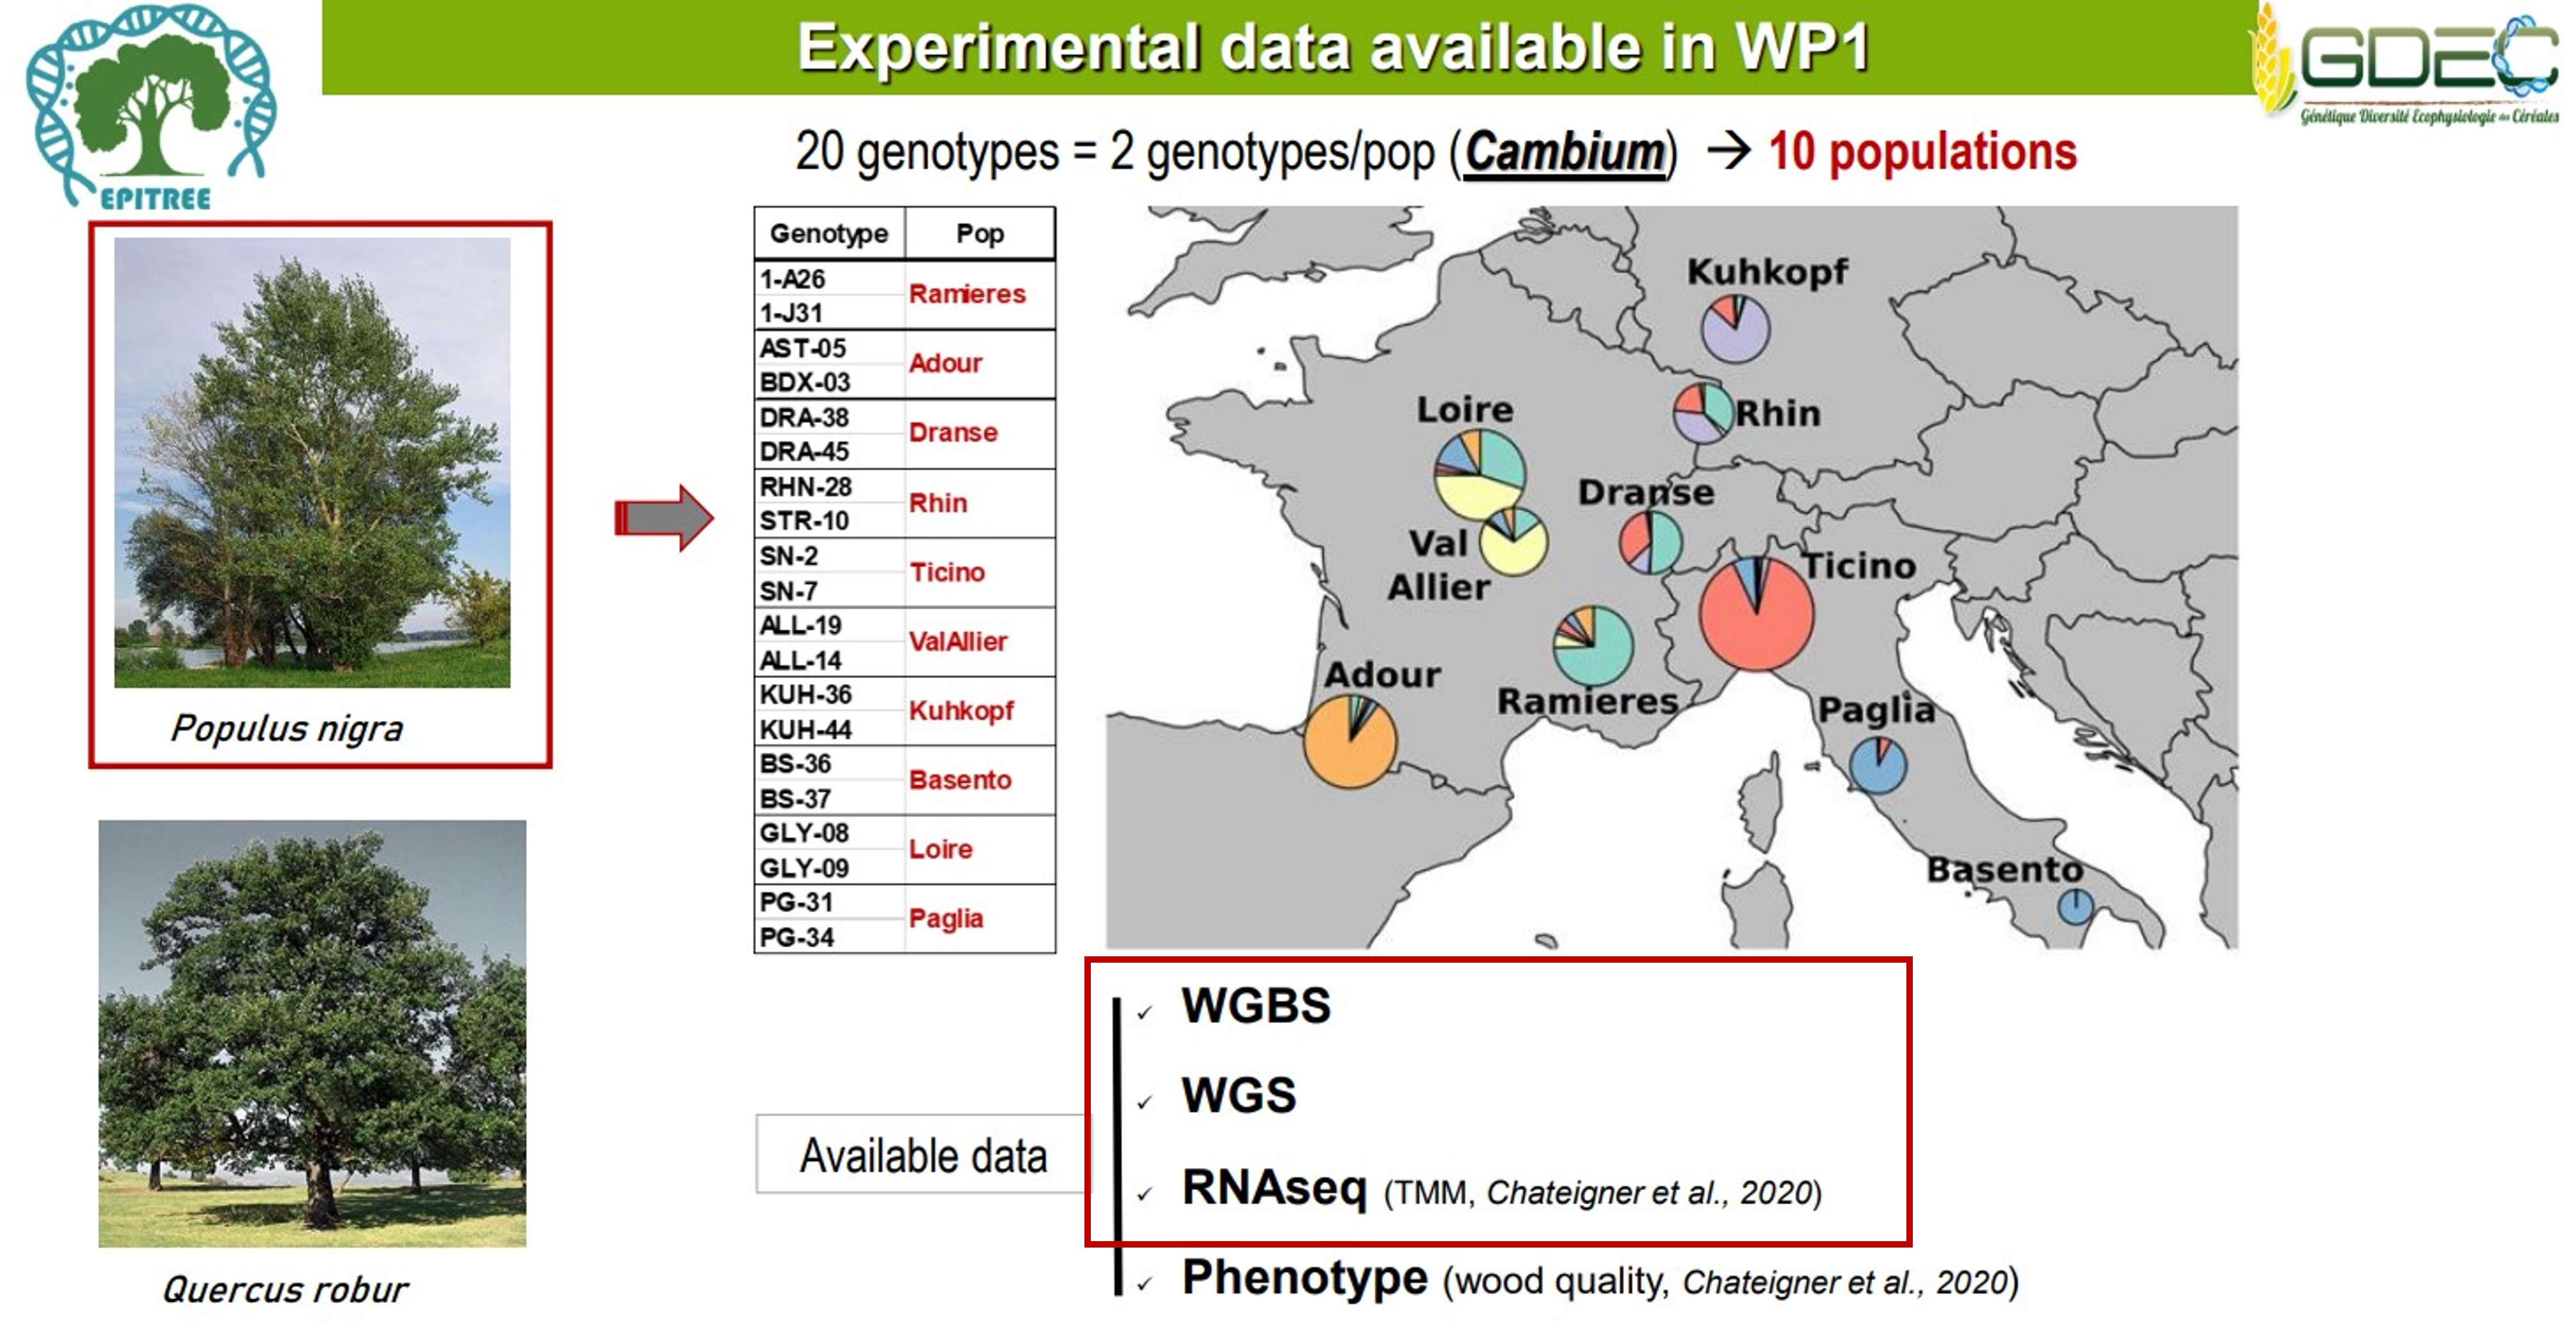
\includegraphics[width=\linewidth]{images/poplar-genotypes.jpg}
\begin{itemize}
\item \emphase{Model tree}: poplar
\item \onslide<2->{$10$ natural populations sampled in Western Europe} 
\item \onslide<3>{$2$ \emphase{genotypes} per population $\rightarrow$ $20$ genotypes.}
\end{itemize}
\begin{figure}[H]
\onslide<1->{
\begin{subfigure}{.25\textwidth}
	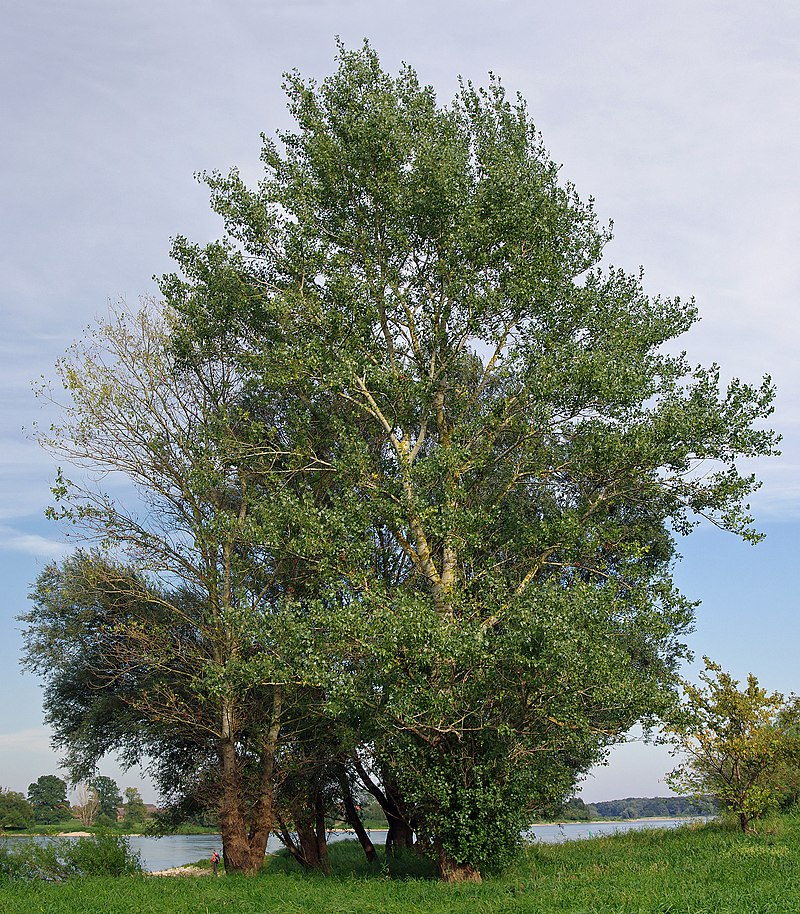
\includegraphics[width=\linewidth]{images/peuplier-noir-Christian-Fischer.jpeg}
	%\caption{\tiny{Poplar; \\ Source: C. Fischer, Wikimedia}}
\end{subfigure}
}
\onslide<2->{
\begin{subfigure}{.45\textwidth}
	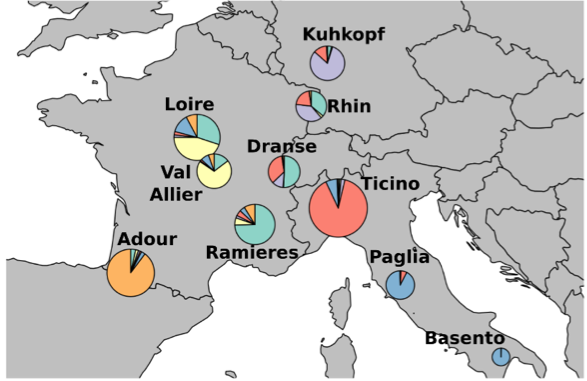
\includegraphics[width=\linewidth]{images/carte-genotypes.png}
\end{subfigure}
}
\caption{Poplar and map of natural populations.}
\end{figure}
\end{frame}

\begin{frame}{Multi-omic data}
Omics measured for $20$ genotypes (\textbf{variables}) for genotype-genotype networks 
\begin{block}{Transcriptomic (\emphase{Gene expression}): \emphase{RNA-Seq} data \citep{chateigner2020gene}}
 \begin{itemize}
\item $34229$ genes (\textbf{samples}).
\item Provided data: continuous and Gaussian. 
\end{itemize}
\end{block}
\begin{block}{Epigenomic (\emphase{DNA methylation}): \emphase{WGBS} data \citep{Sow2022Landscape}} 
\only<4>{
\centering
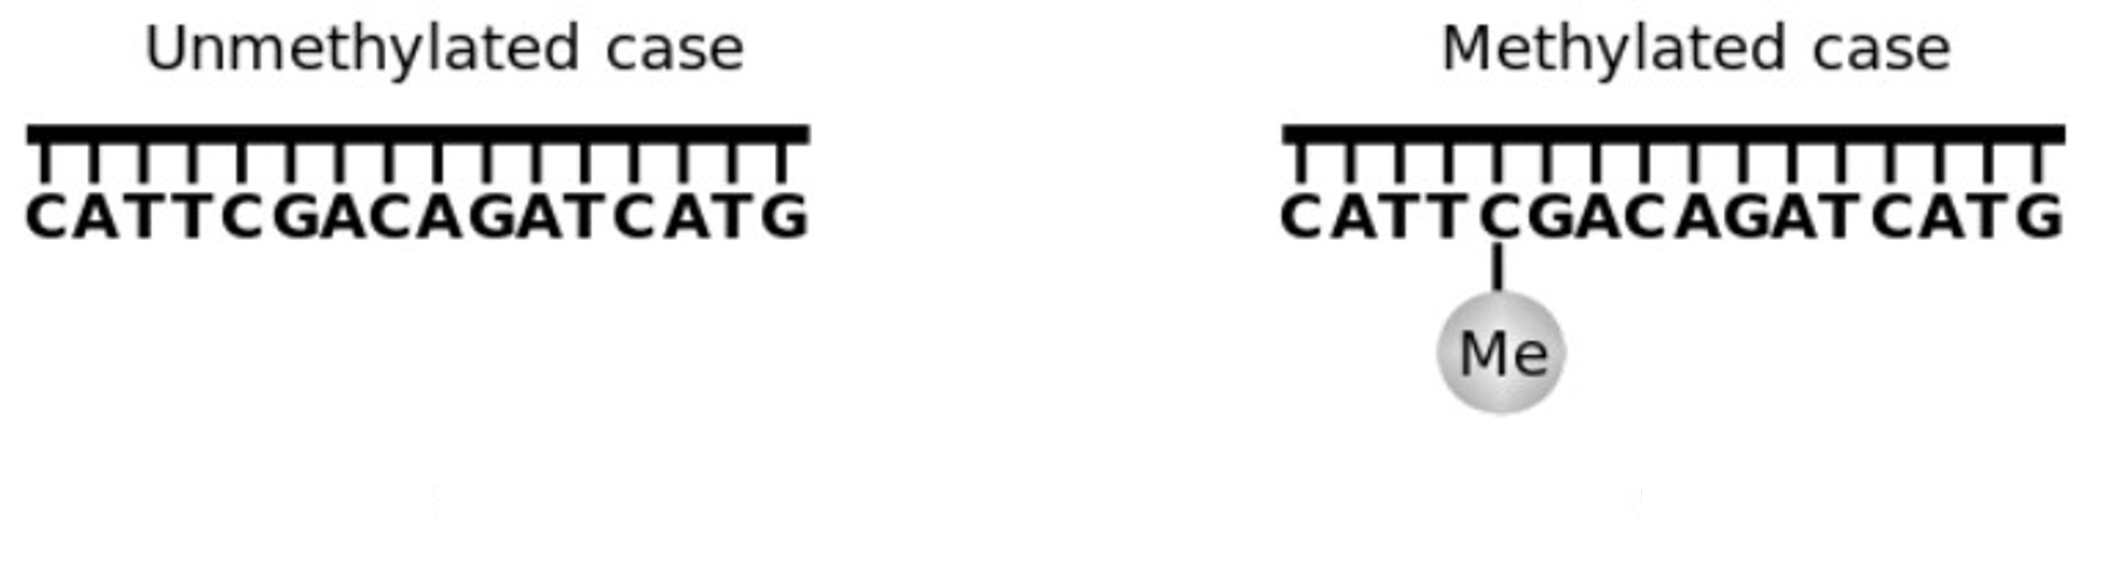
\includegraphics[width=0.8\linewidth]{images/unmethyl-methyl.png}}

\only<5>{
\centering
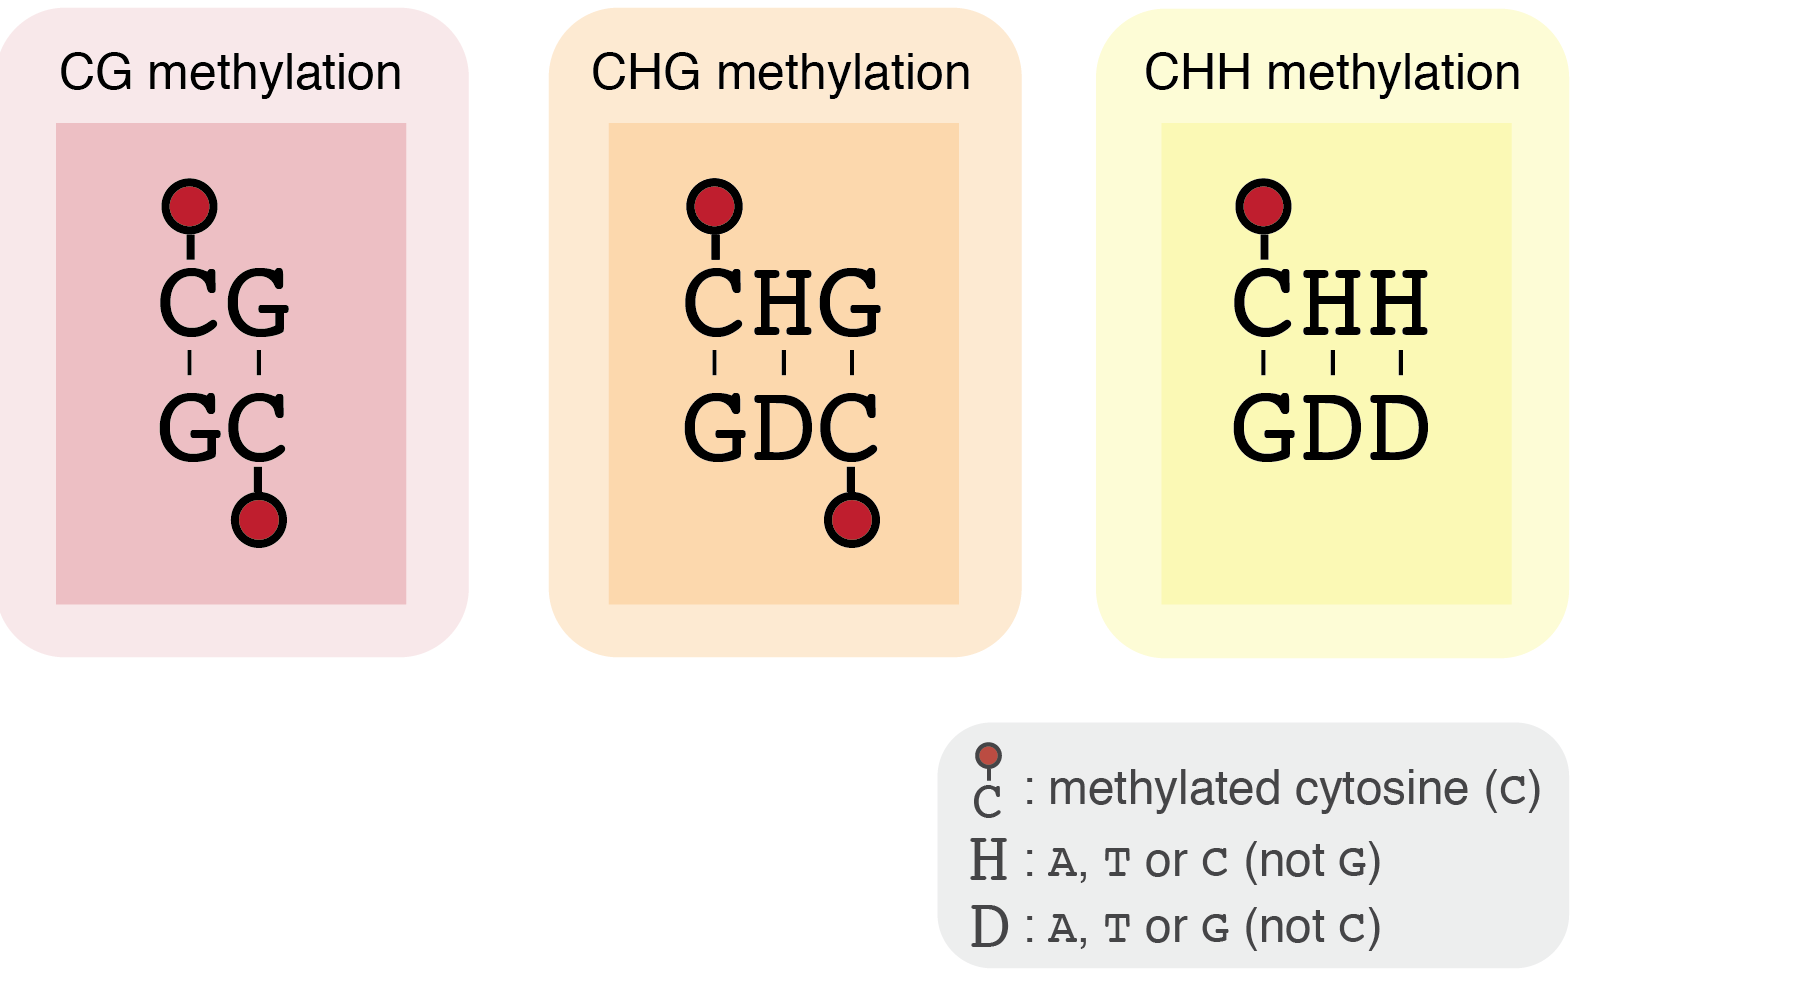
\includegraphics[width=7cm]{images/Methylation_context.png}
}

\only<6>{
\centering
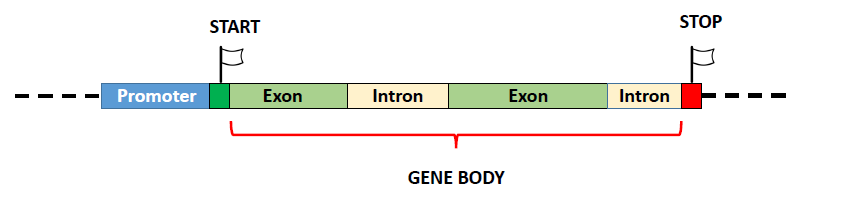
\includegraphics[width=8cm]{images/gene-body-promoter.png}
}
\begin{itemize} 
\onslide<7->{\item Three \emphase{methylation contexts} measured on \emphase{gene-body and gene-promoter}.
	\item $\rightarrow 6$ data-sets each containing about $40000$ genes (\textbf{samples}). } 
\onslide<8->{\item Provided data: normalized counts per gene.
	\item To gaussian: $log_2(x+1)$ with $x \in \mathbb R.$}
	\end{itemize}
\end{block}
\onslide<9>{For each omic, average measures per natural populations.}
\end{frame}



\subsection{Genotype x Genotype networks}

\begin{frame}{Complex omics data integration}

\centering
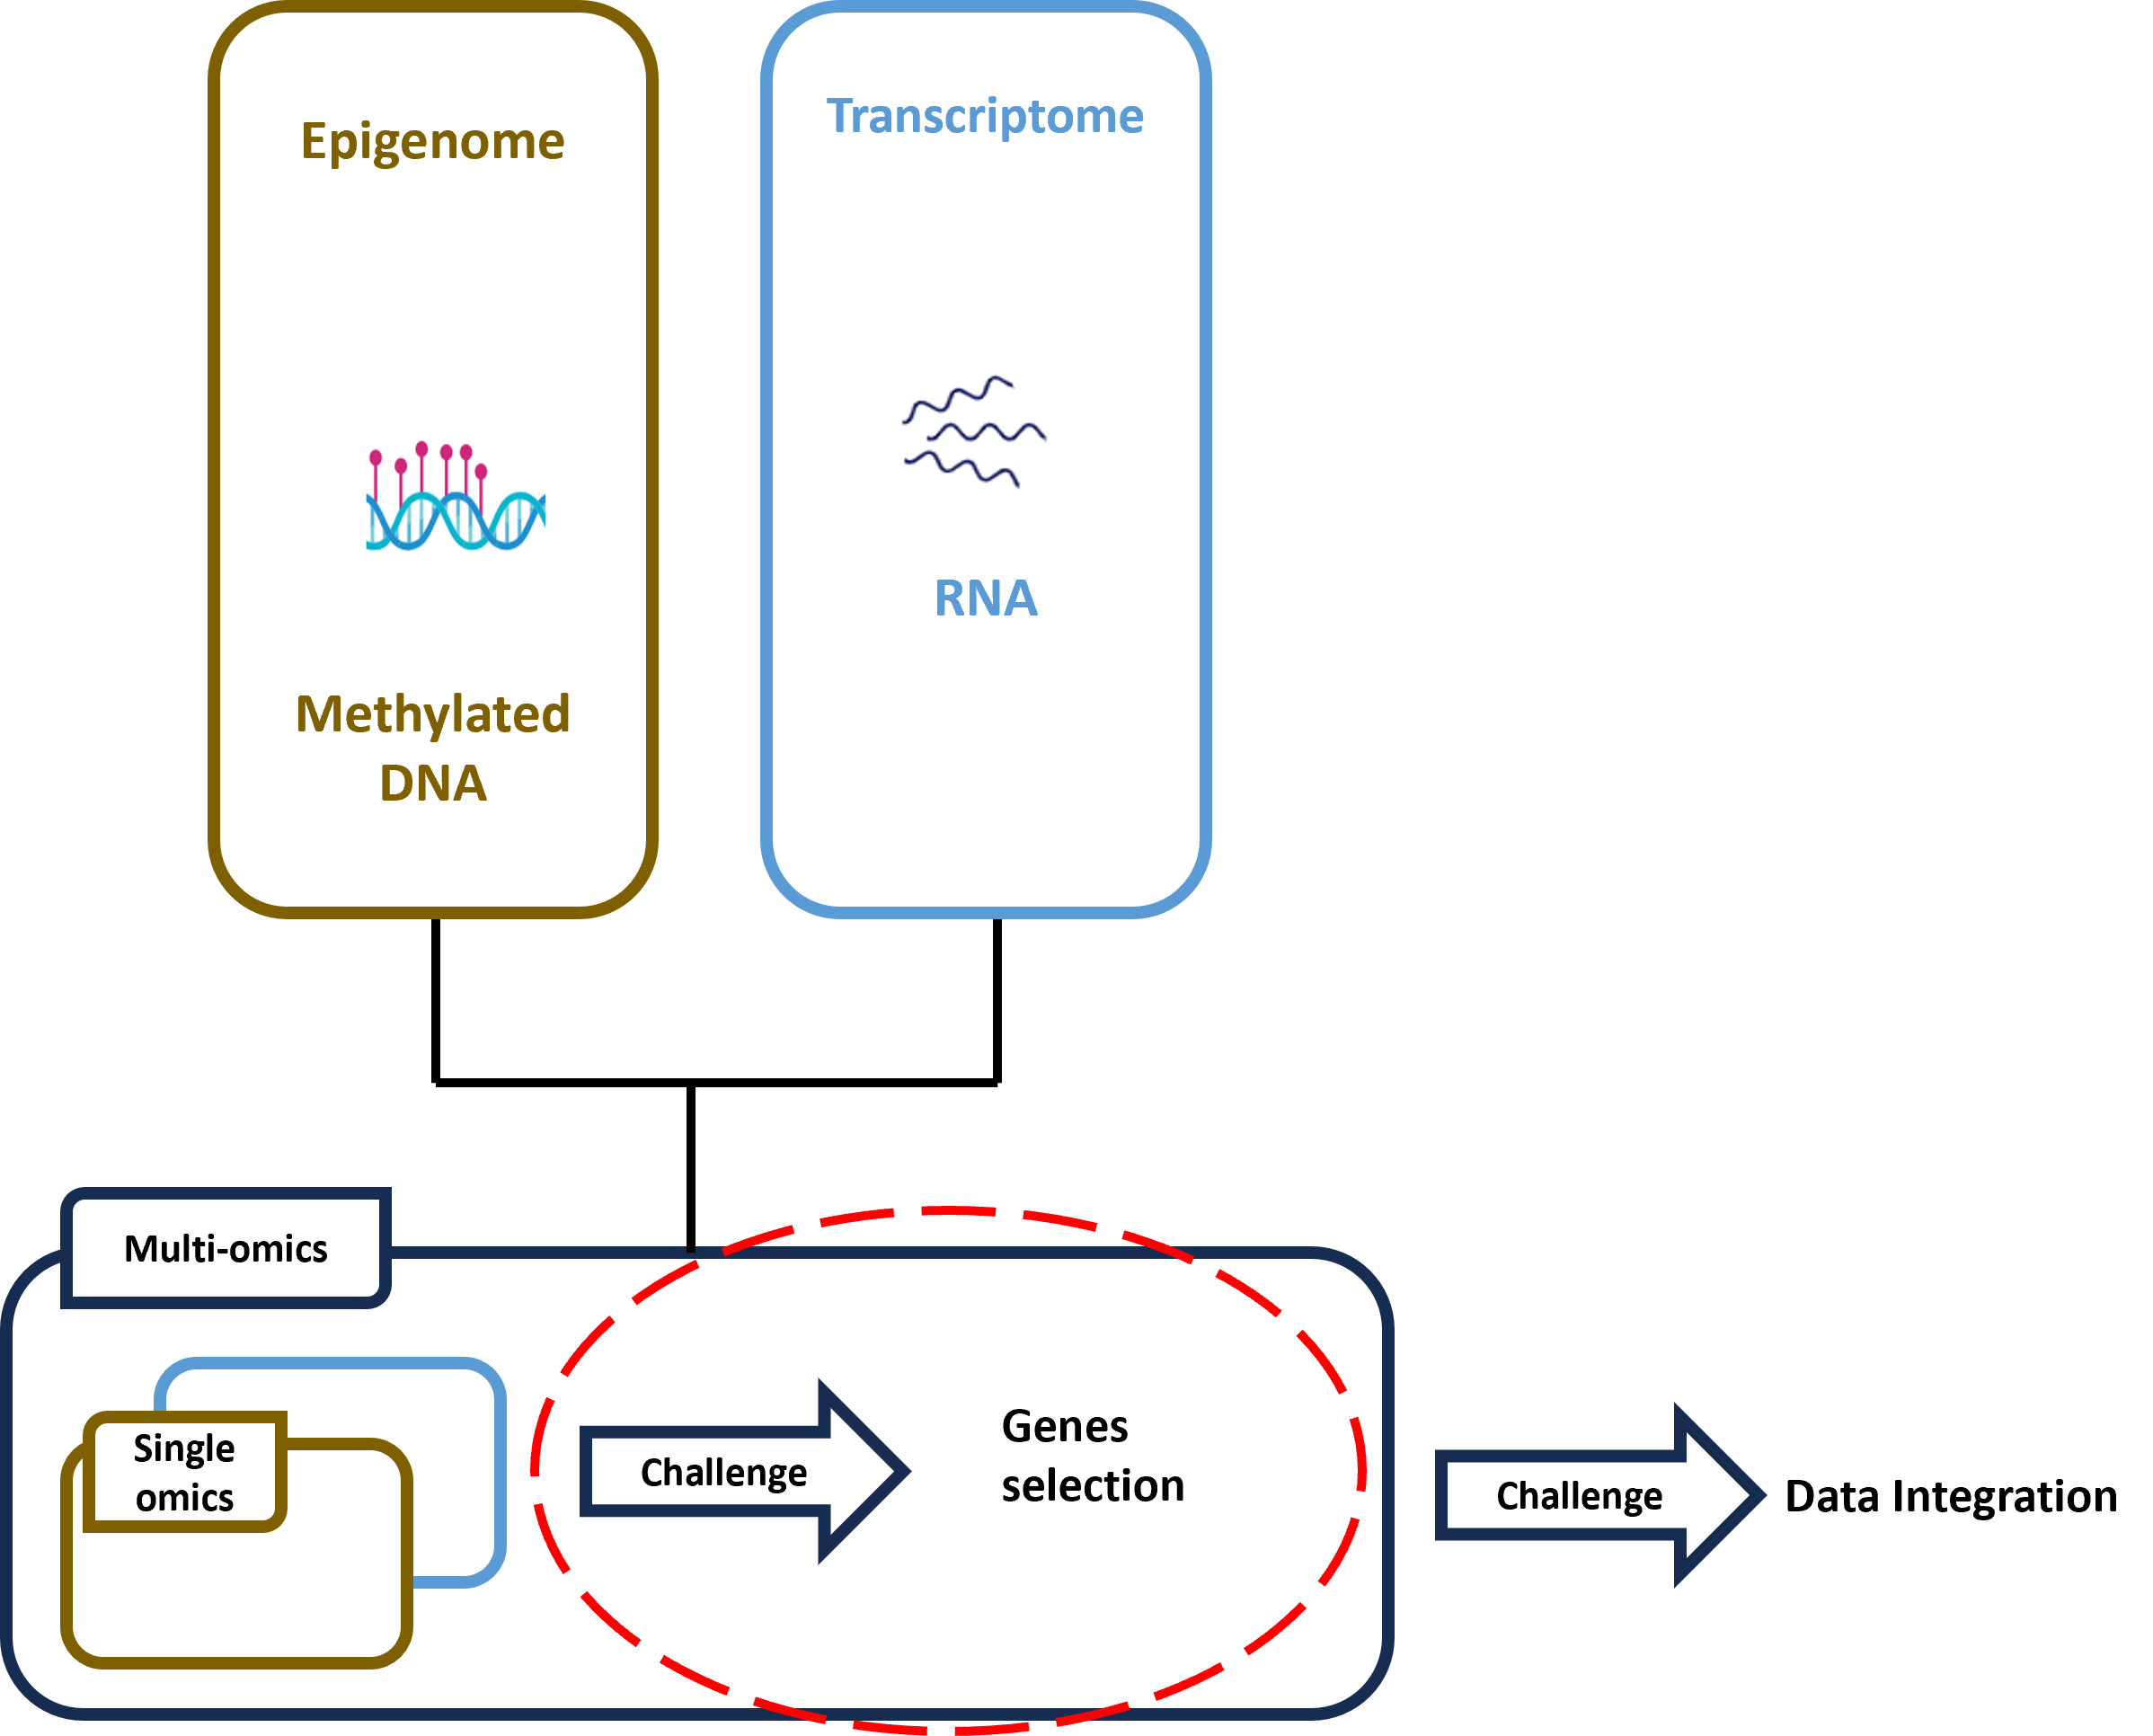
\includegraphics[width=5cm]{images/epigenome-transcriptome-feature-selection.png}

\begin{block}{Genes (\textbf{samples}) selection }
\begin{itemize}
\item For scalability issue of MGLASSO. 
\item For each omic data, apply \emphase{sparse PCA} and select $15$ top-genes for the $3$ PCs using \texttt{mixomics}.
\item Merge genes lists for all the omics and remove duplicates: $151$ genes.
\end{itemize}
\end{block}
\end{frame}

\begin{frame}{Integration across genes}
\centering
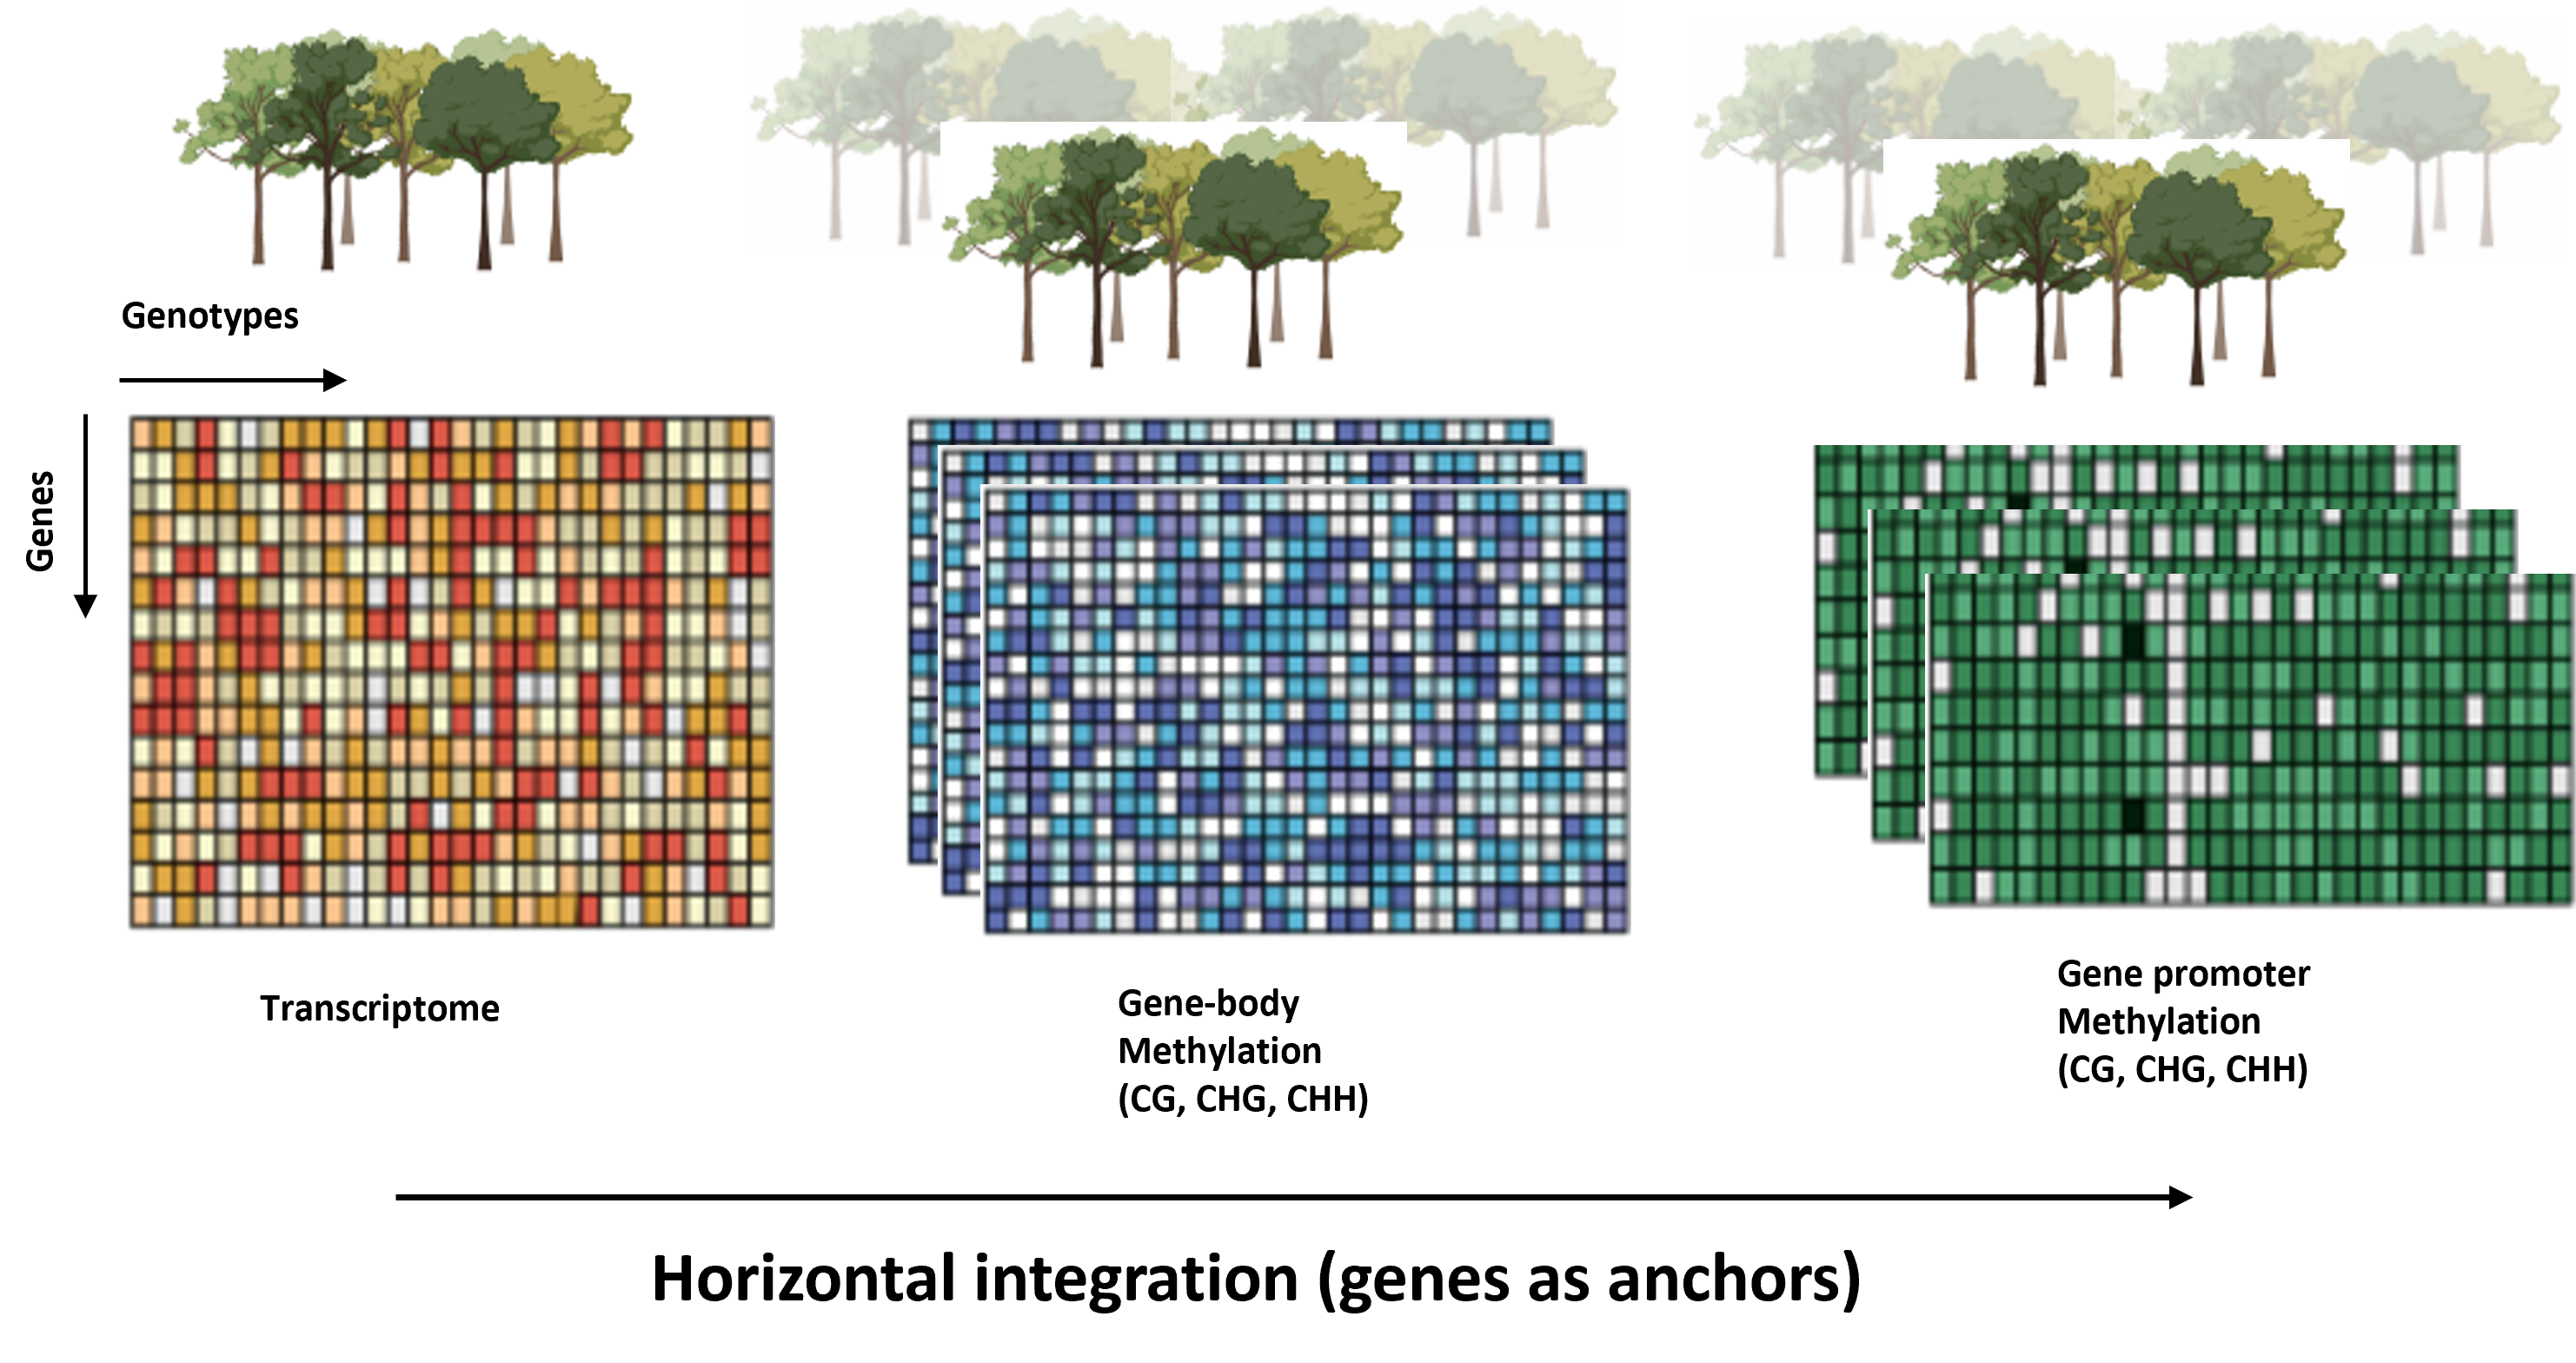
\includegraphics[width=7cm]{images/horizontal-integration-after-slection.png}

\begin{itemize}
\item $\mathbf X: 151$ (genes) observations of $70$ Gaussian methylation and transcriptomic profiles (variables)
\end{itemize}
\end{frame}



\begin{frame}{Clustering path}
MGLASSO identifies \emphase{three coherent groups} of omics profiles.
%merge
%\begin{columns}
%\begin{column}{0.7\textwidth}
\begin{figure}
\centering
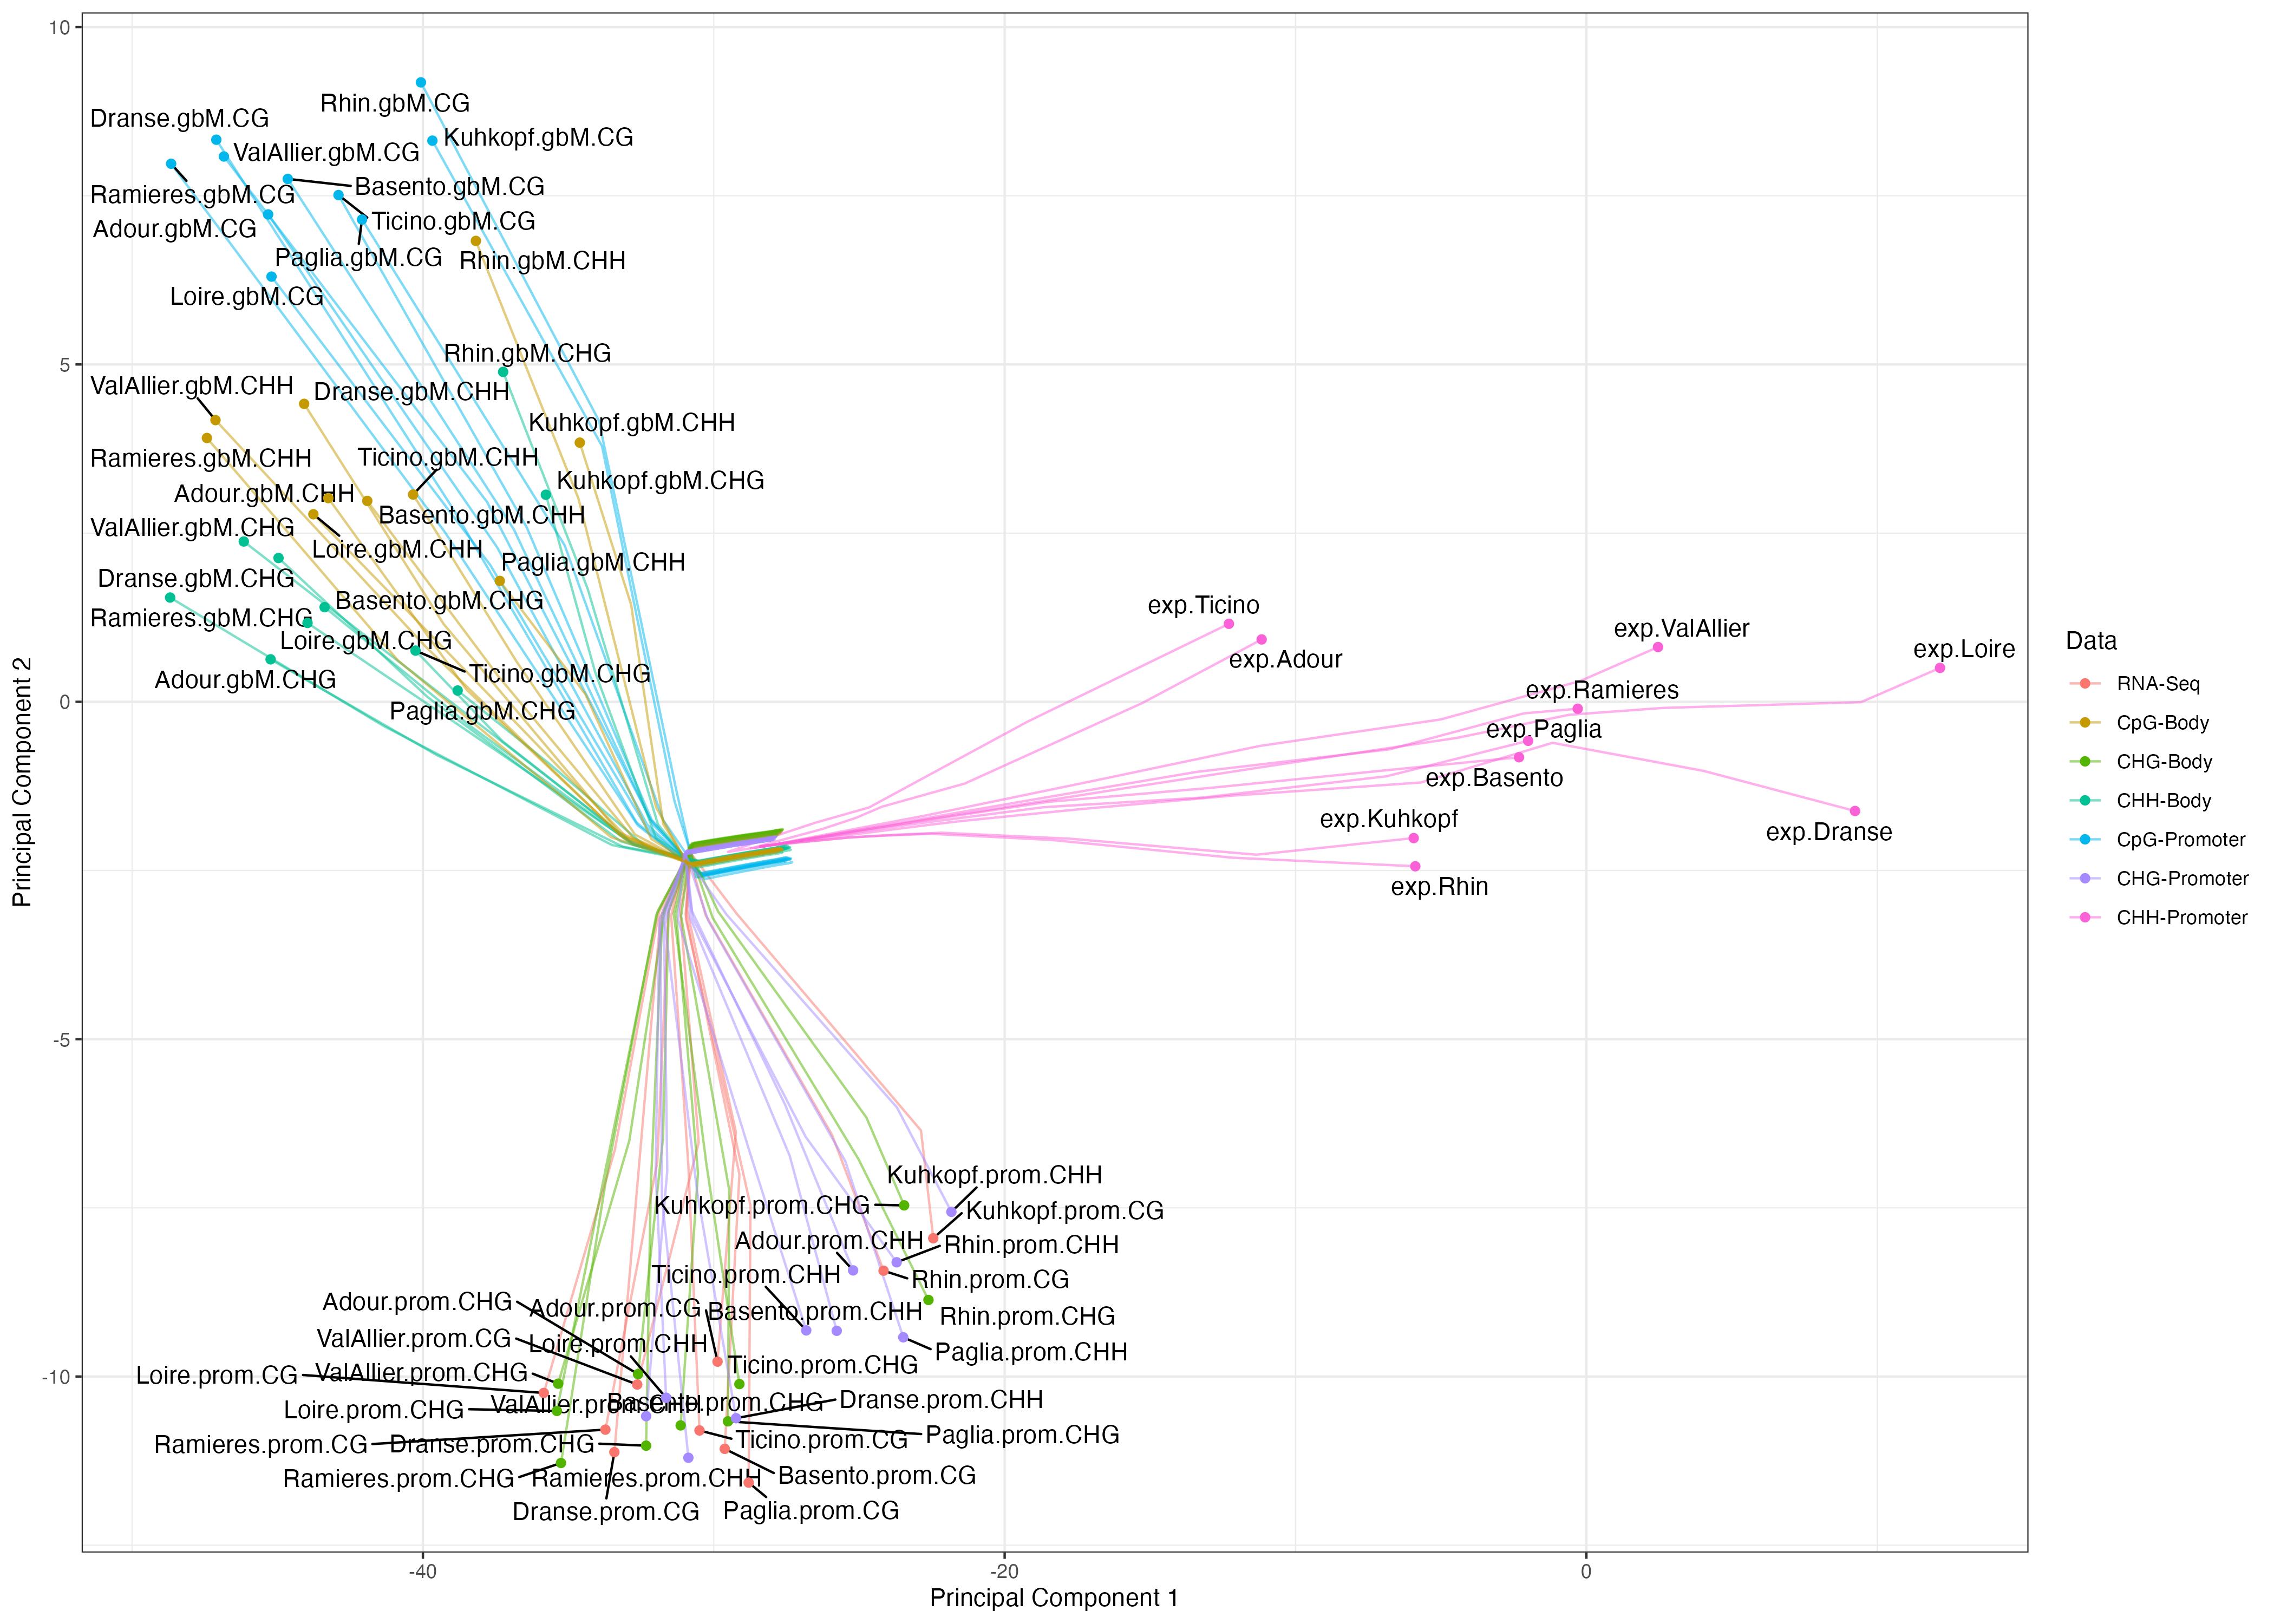
\includegraphics[width=0.85\linewidth]{images/cuttree-clusterpath-path-poplar-exp-meth.png}
\end{figure}
%\end{column}


\end{frame}

\begin{frame}{Multiscale Networks: non-compressed view (1)}
%\only<1>{
\begin{figure}
\centering
\subfloat[$\lambda_2$ = 0]{\label{fig:adj_mat_mglasso_epitree1}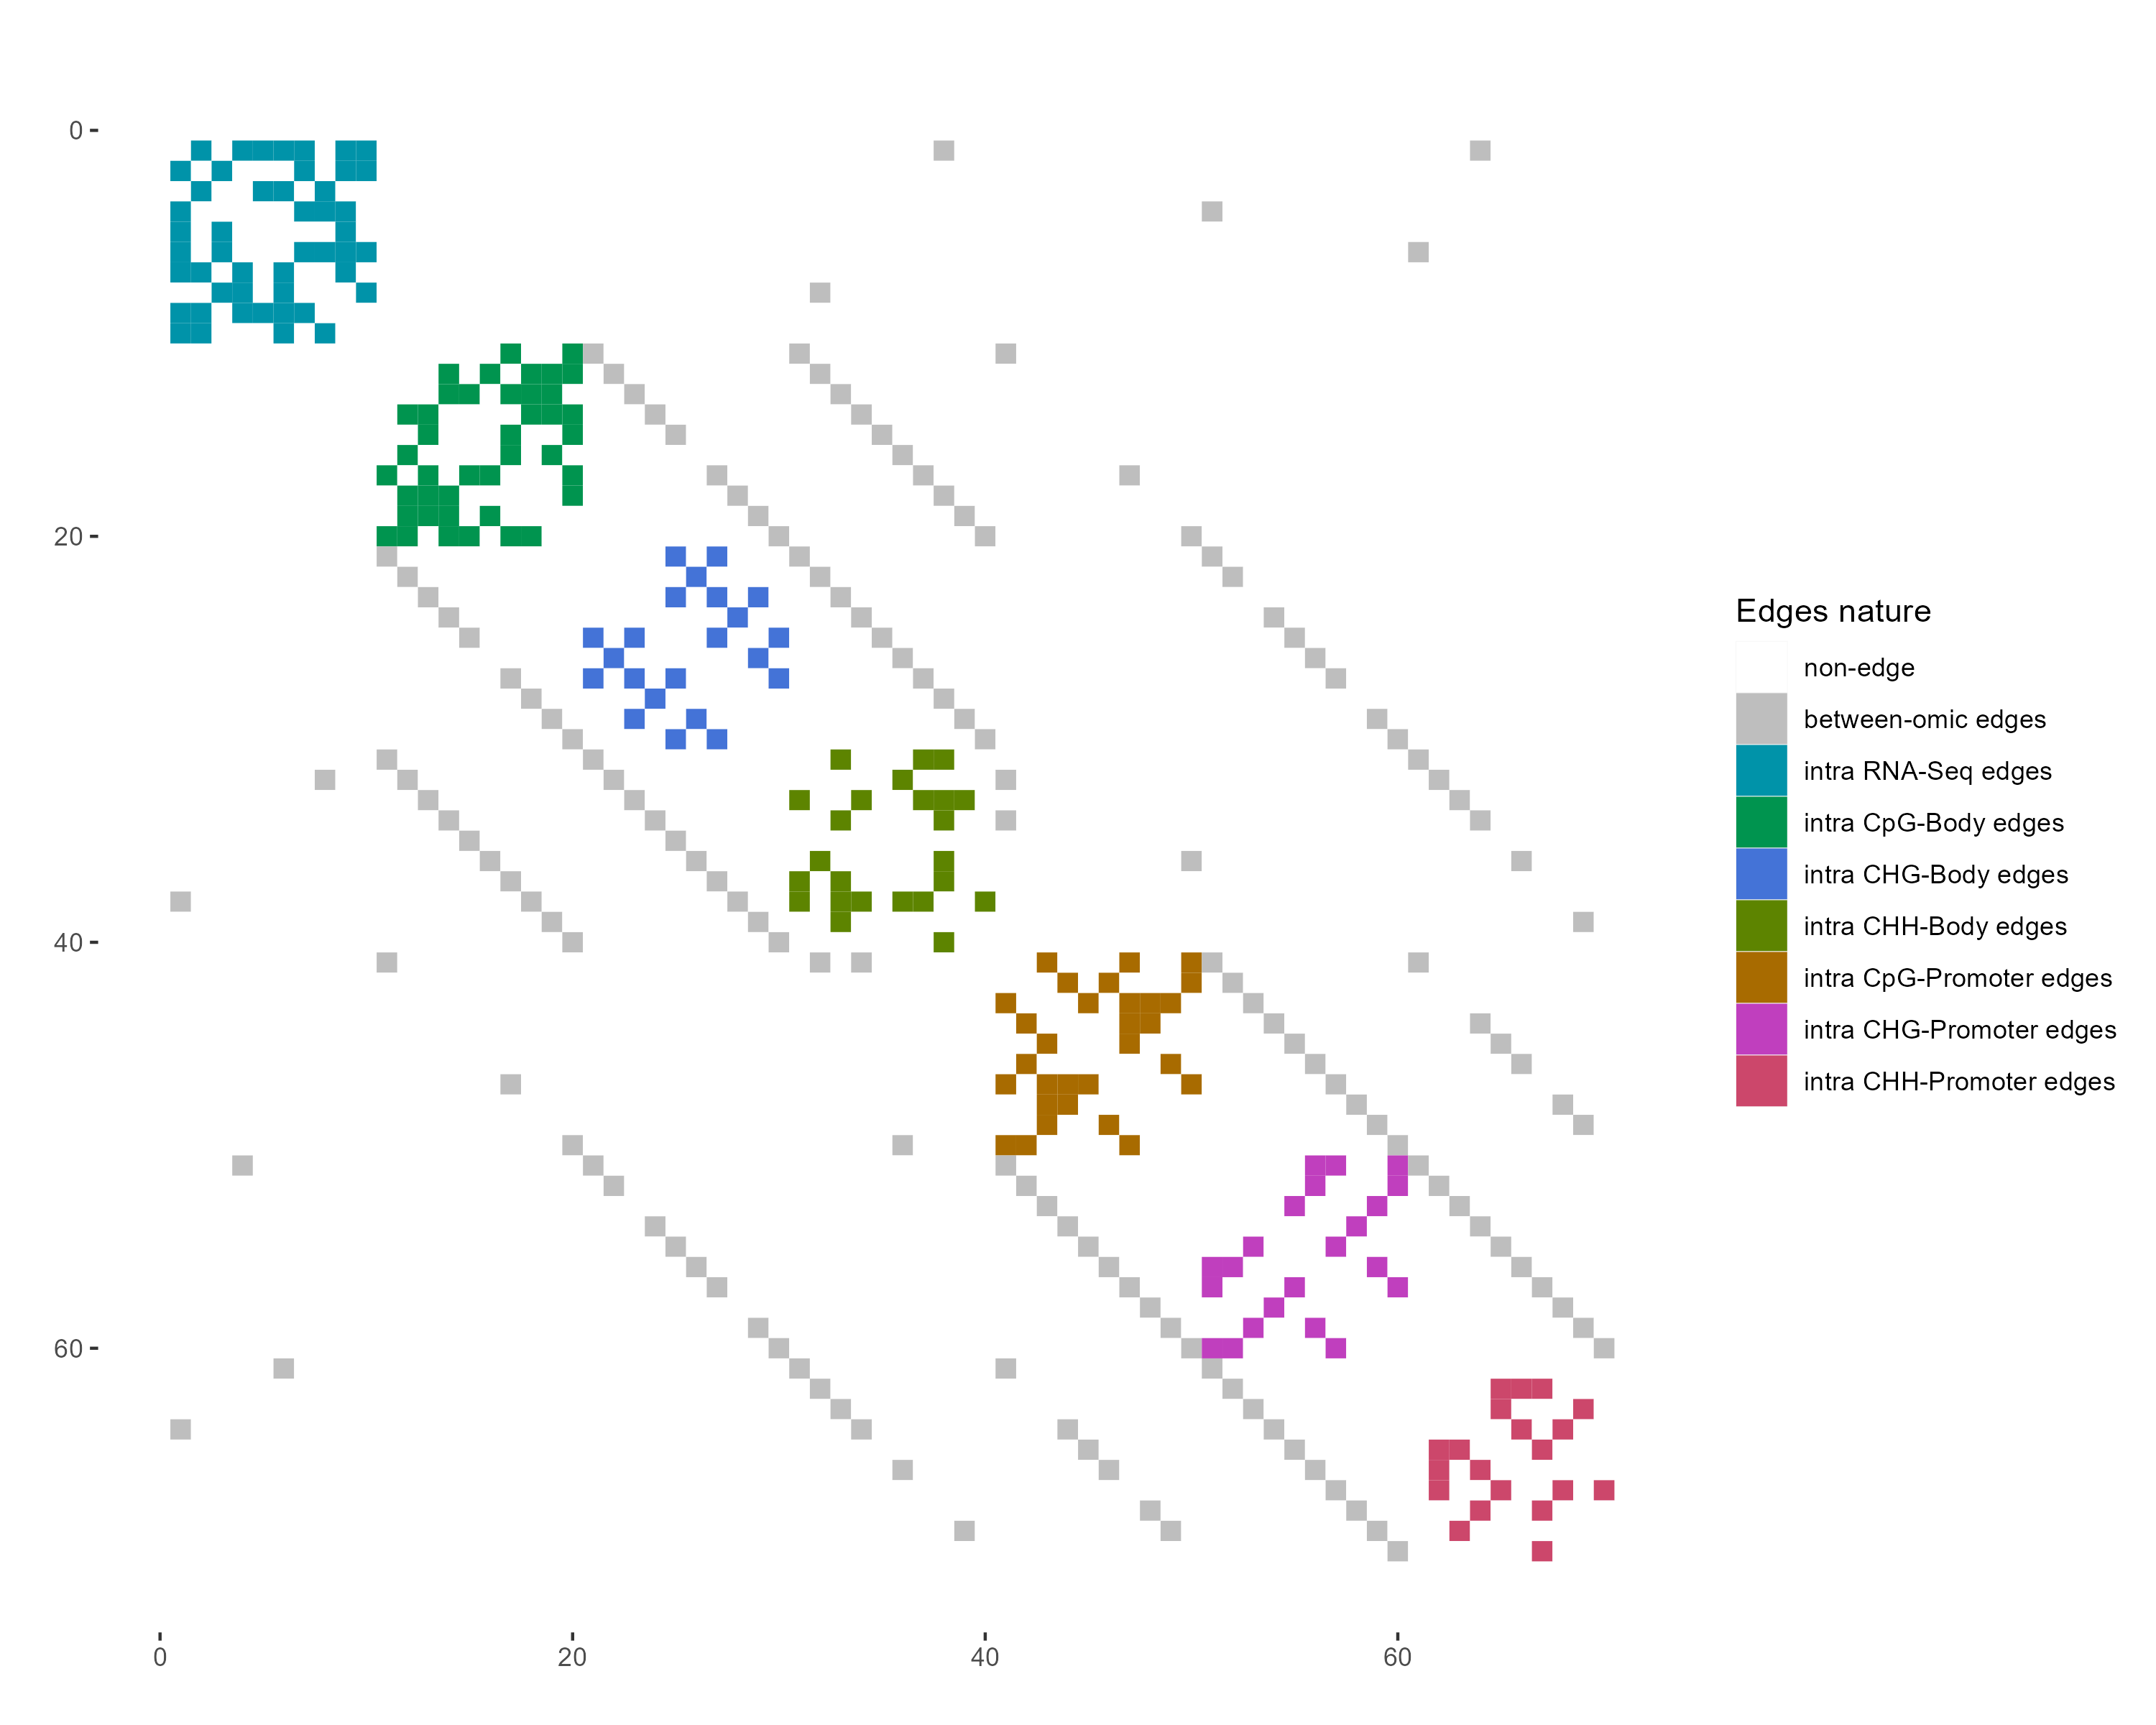
\includegraphics[height=7cm]{images/colored-adj_mat_mglasso_genot1_order_omic.png}}
\end{figure}



\end{frame}

\begin{frame}{Multiscale Networks: non-compressed view (2)}
\begin{figure}
\centering
\begin{subfigure}{0.4\linewidth}
\centering
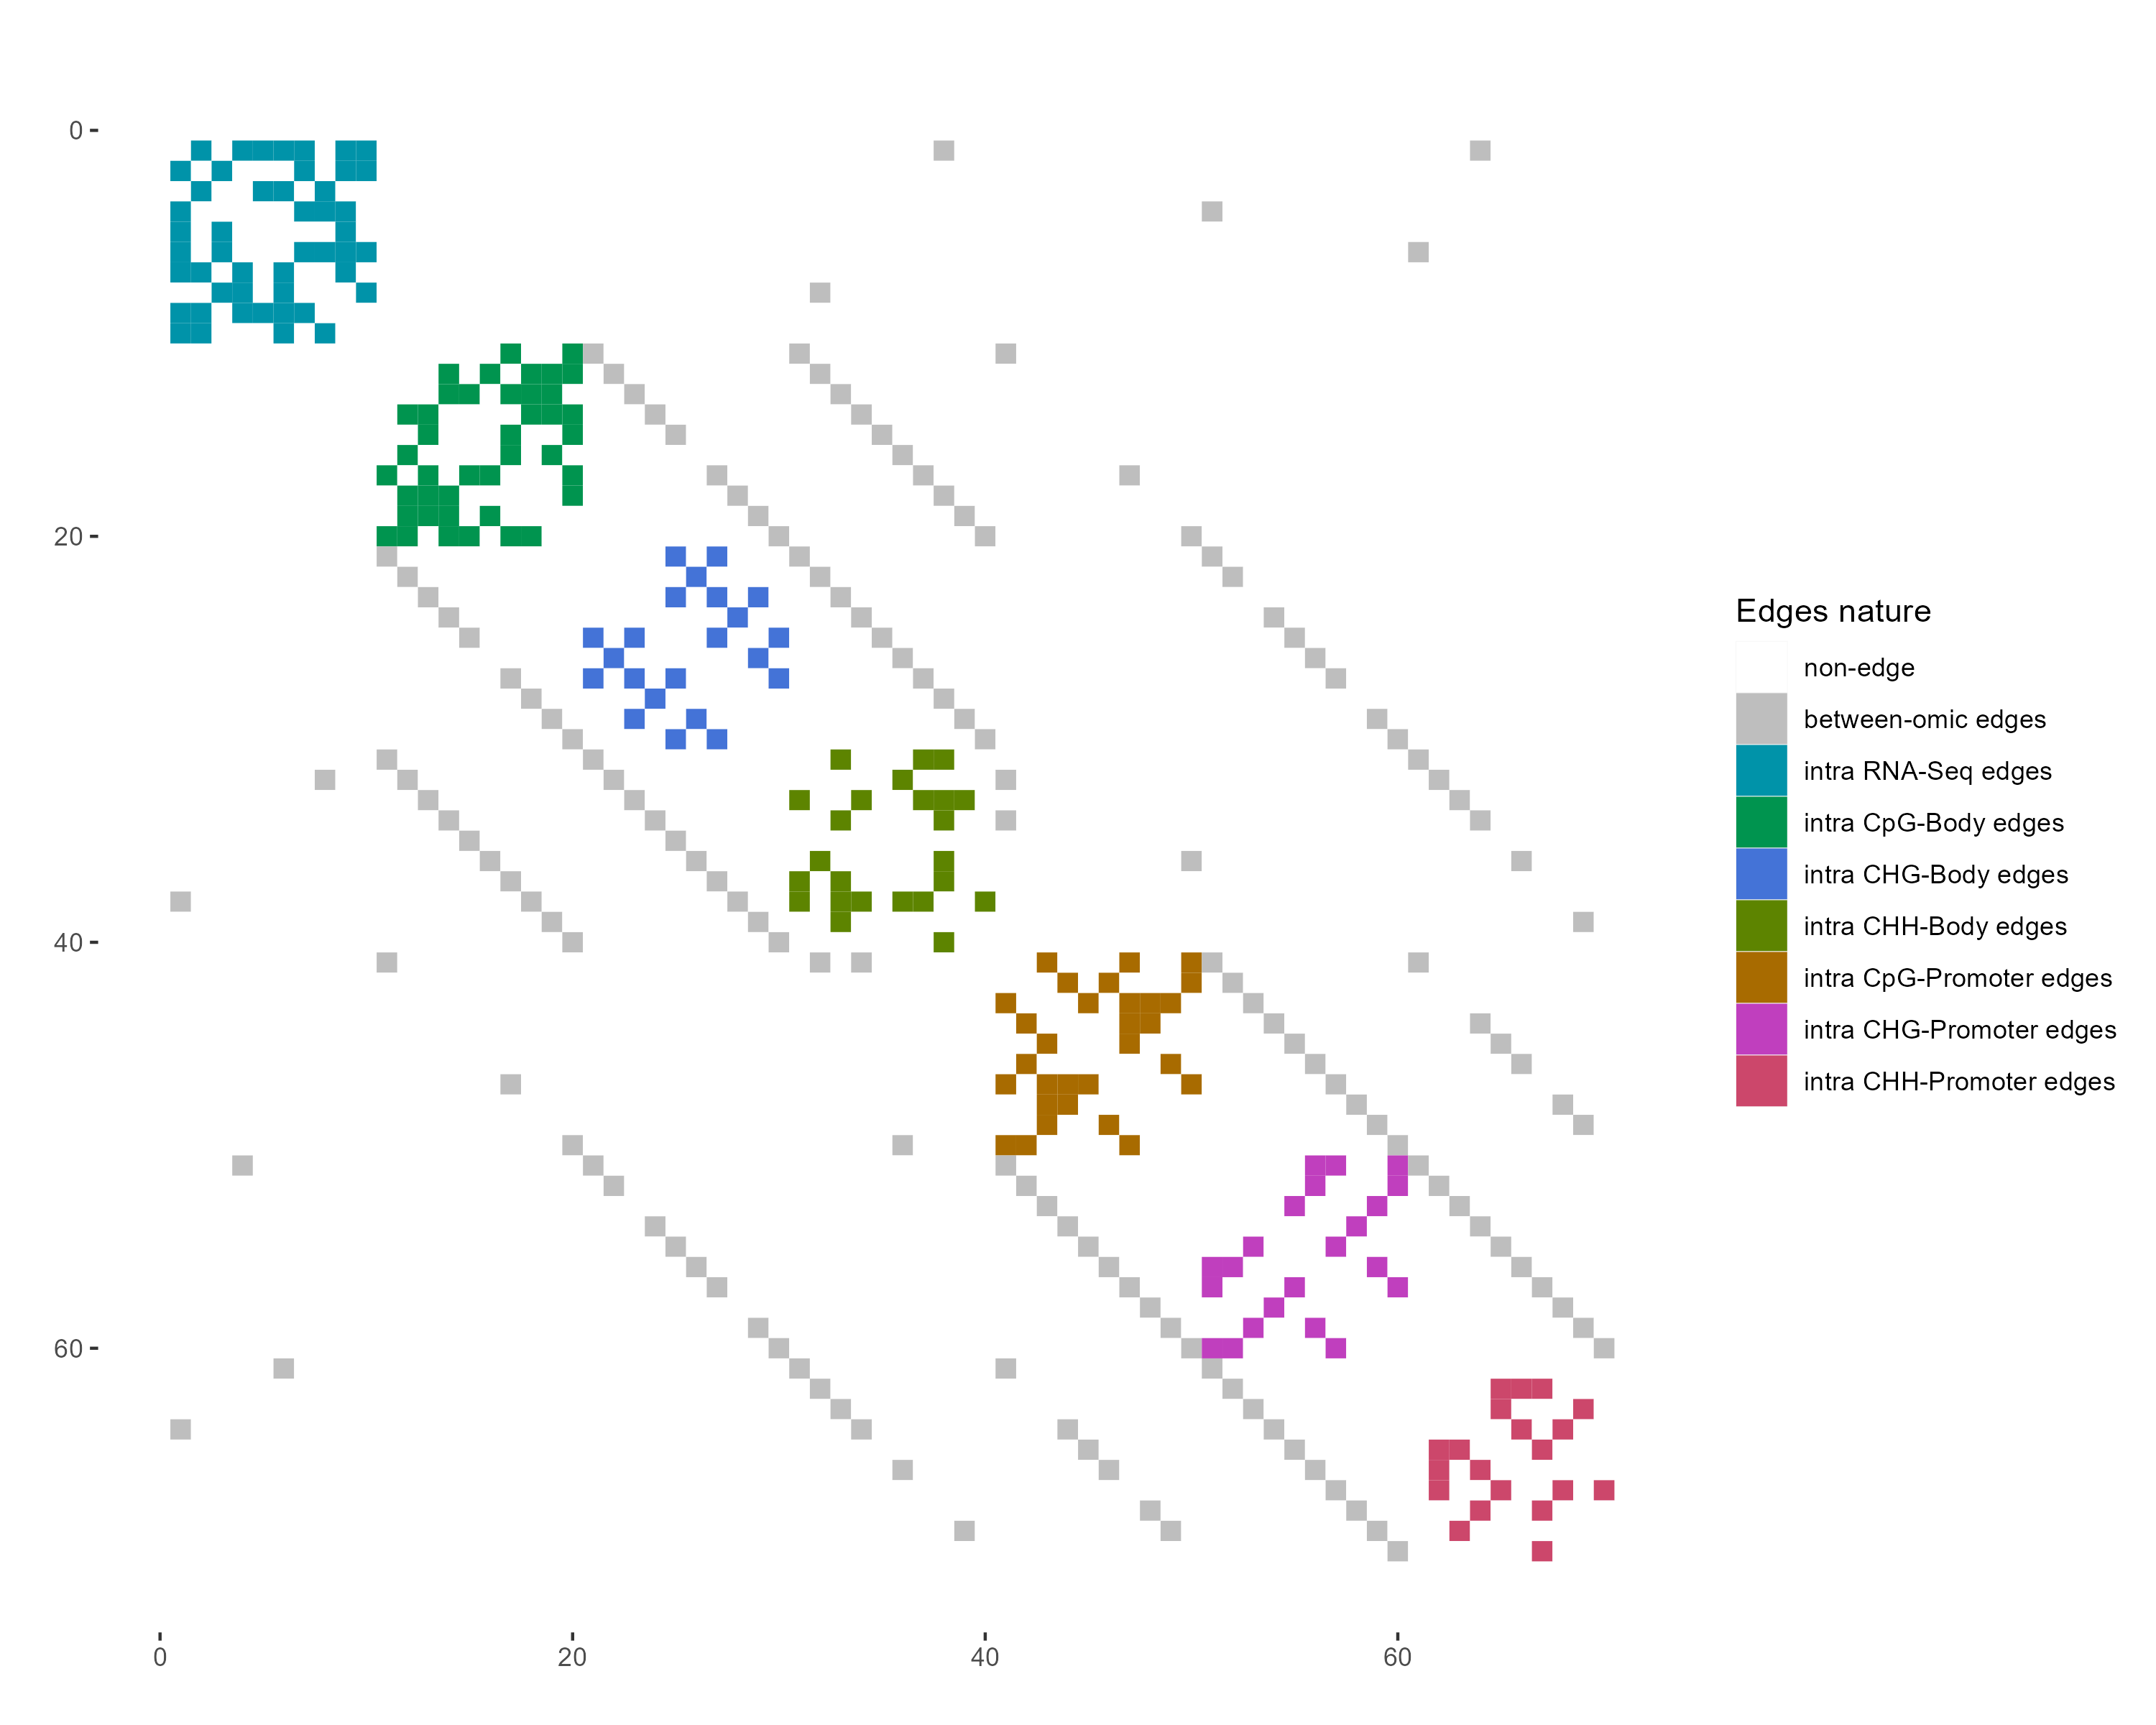
\includegraphics[scale = 0.14]{images/colored-adj_mat_mglasso_genot1_order_omic.png}
\caption{$\lambda_2$ = 0}
\end{subfigure}
\hfill
\begin{subfigure}{0.4\linewidth}
\centering
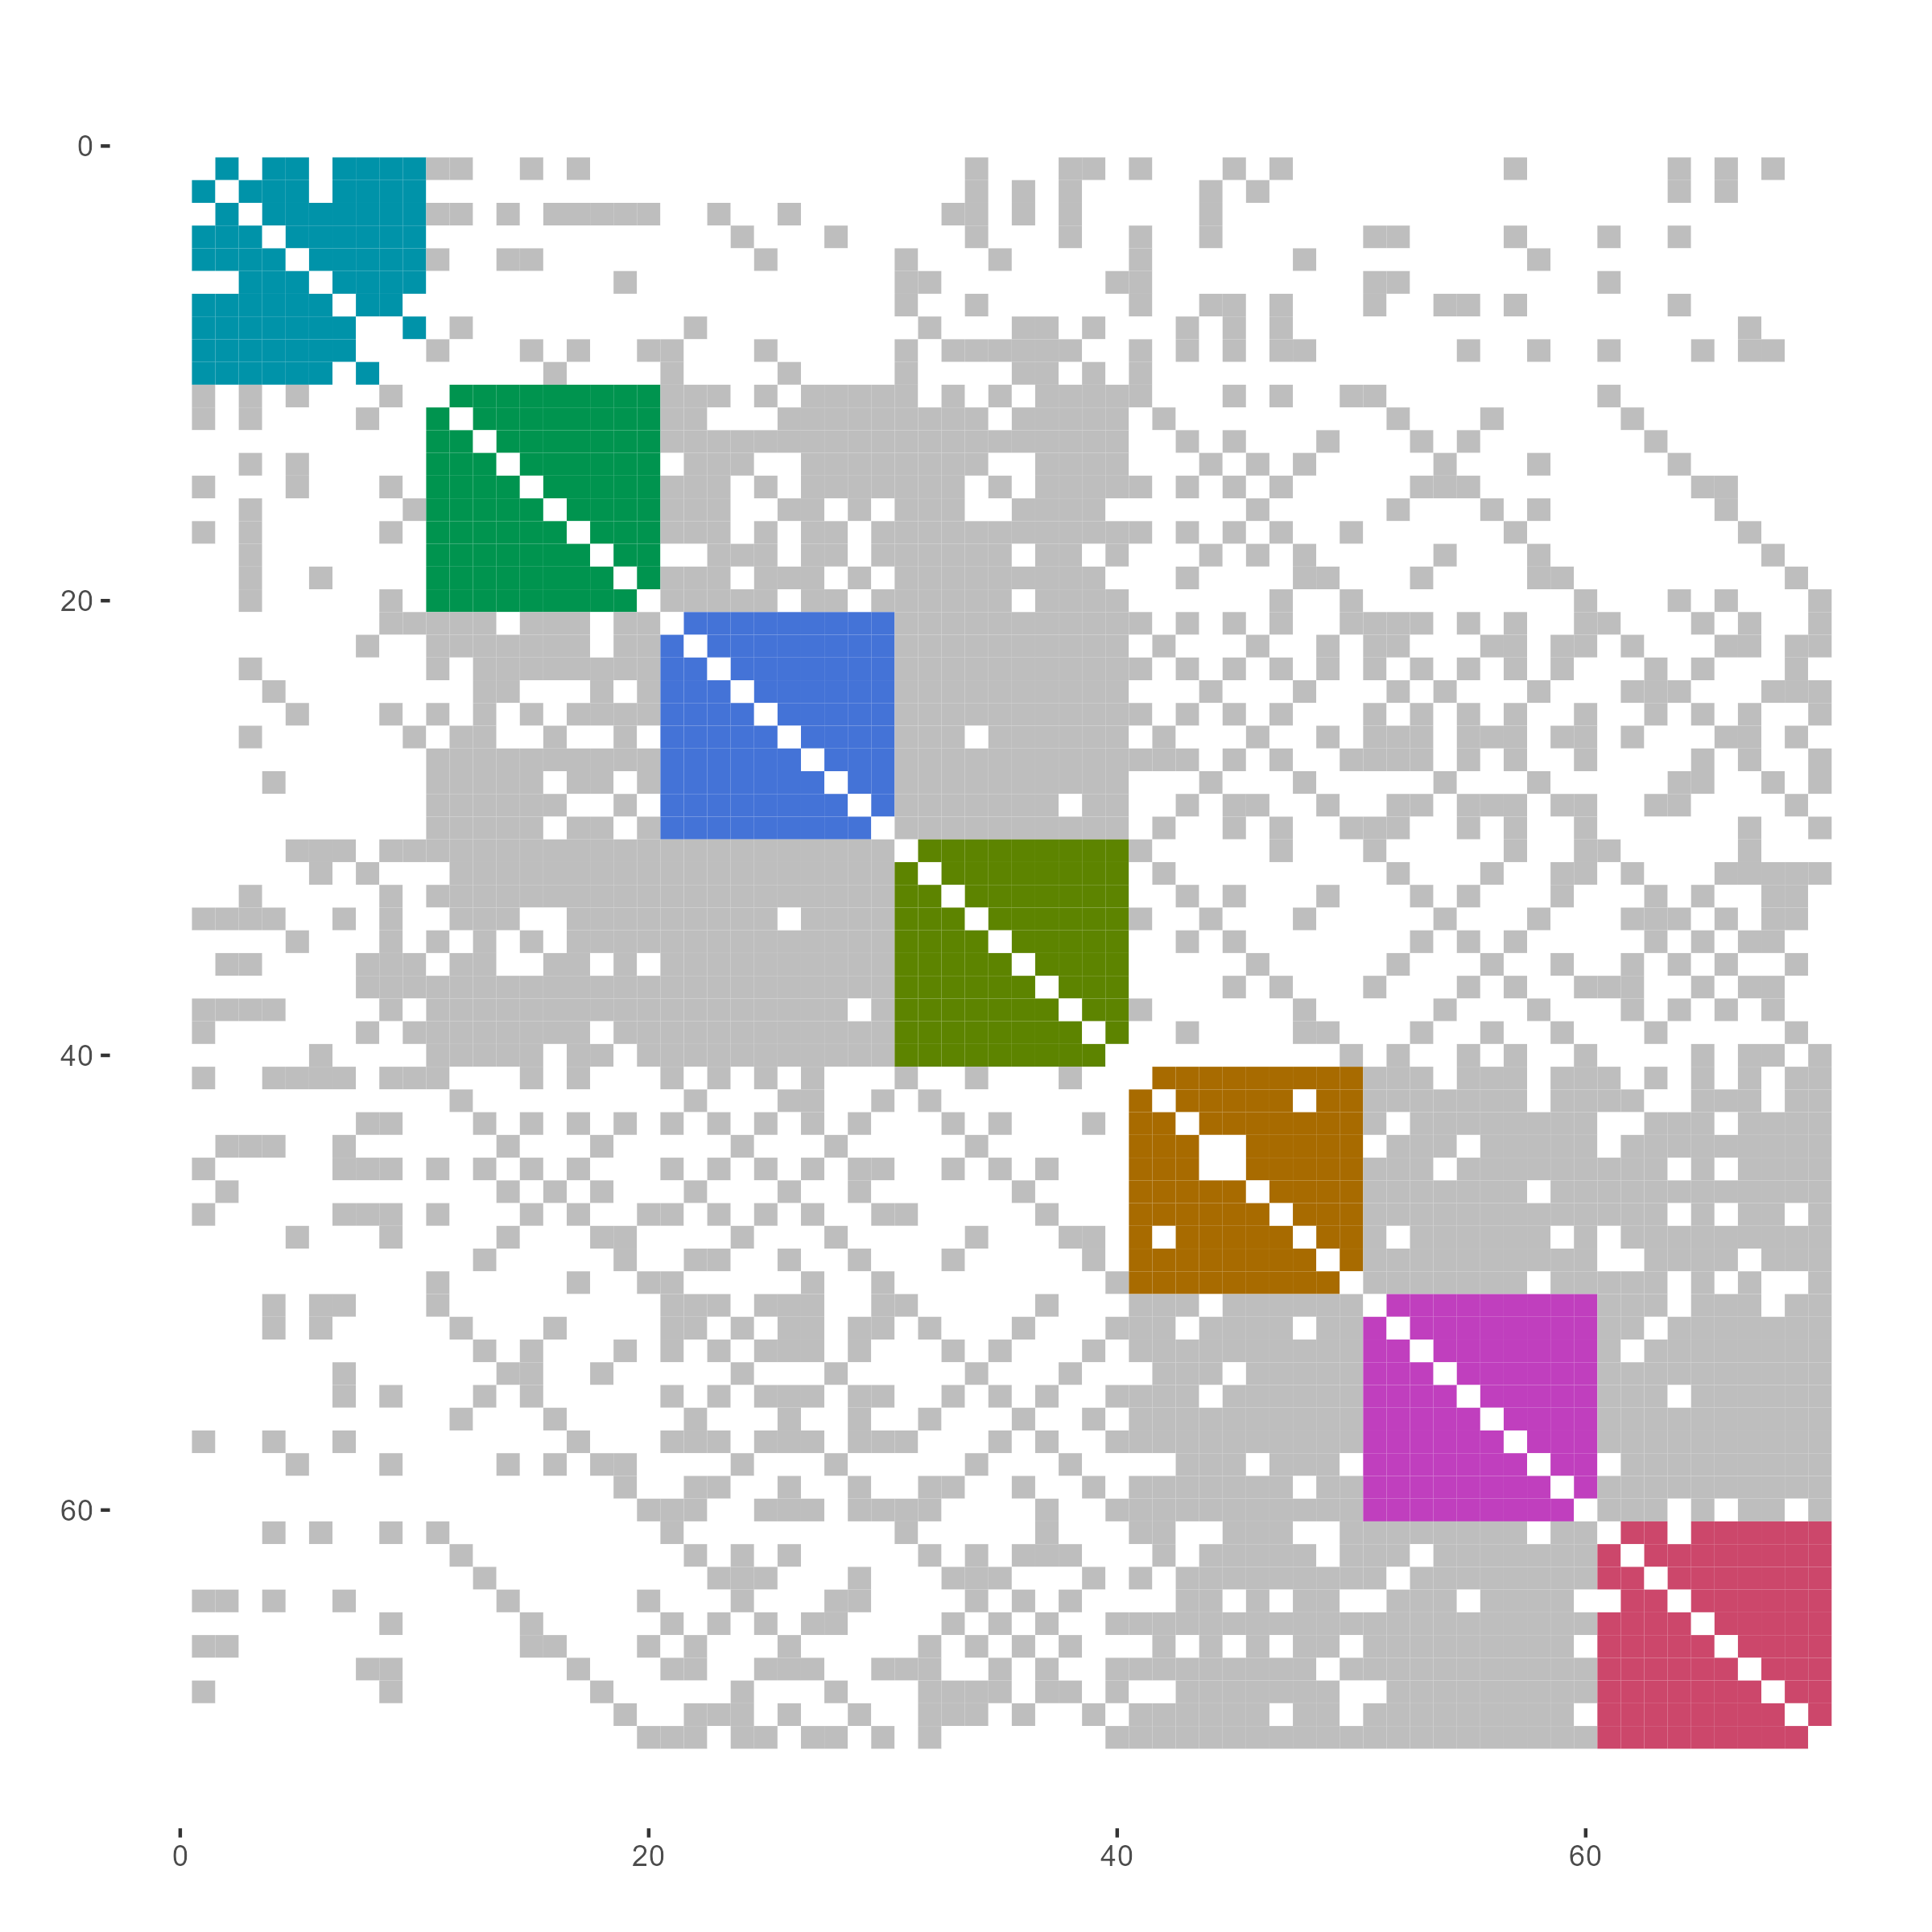
\includegraphics[scale = 0.14]{images/colored-adj_mat_mglasso_genot2_order_omic.png}
\caption{$\lambda_2$ = 1.63}
\end{subfigure}
\hfill
%	\begin{subfigure}{0.3\linewidth}
%		%\centering
%		%\includegraphics[width=\linewidth]{subfig6}
%		%\caption{Subfigure 6}
%	\end{subfigure}
%\hfill
\begin{subfigure}{0.3\linewidth}
\centering
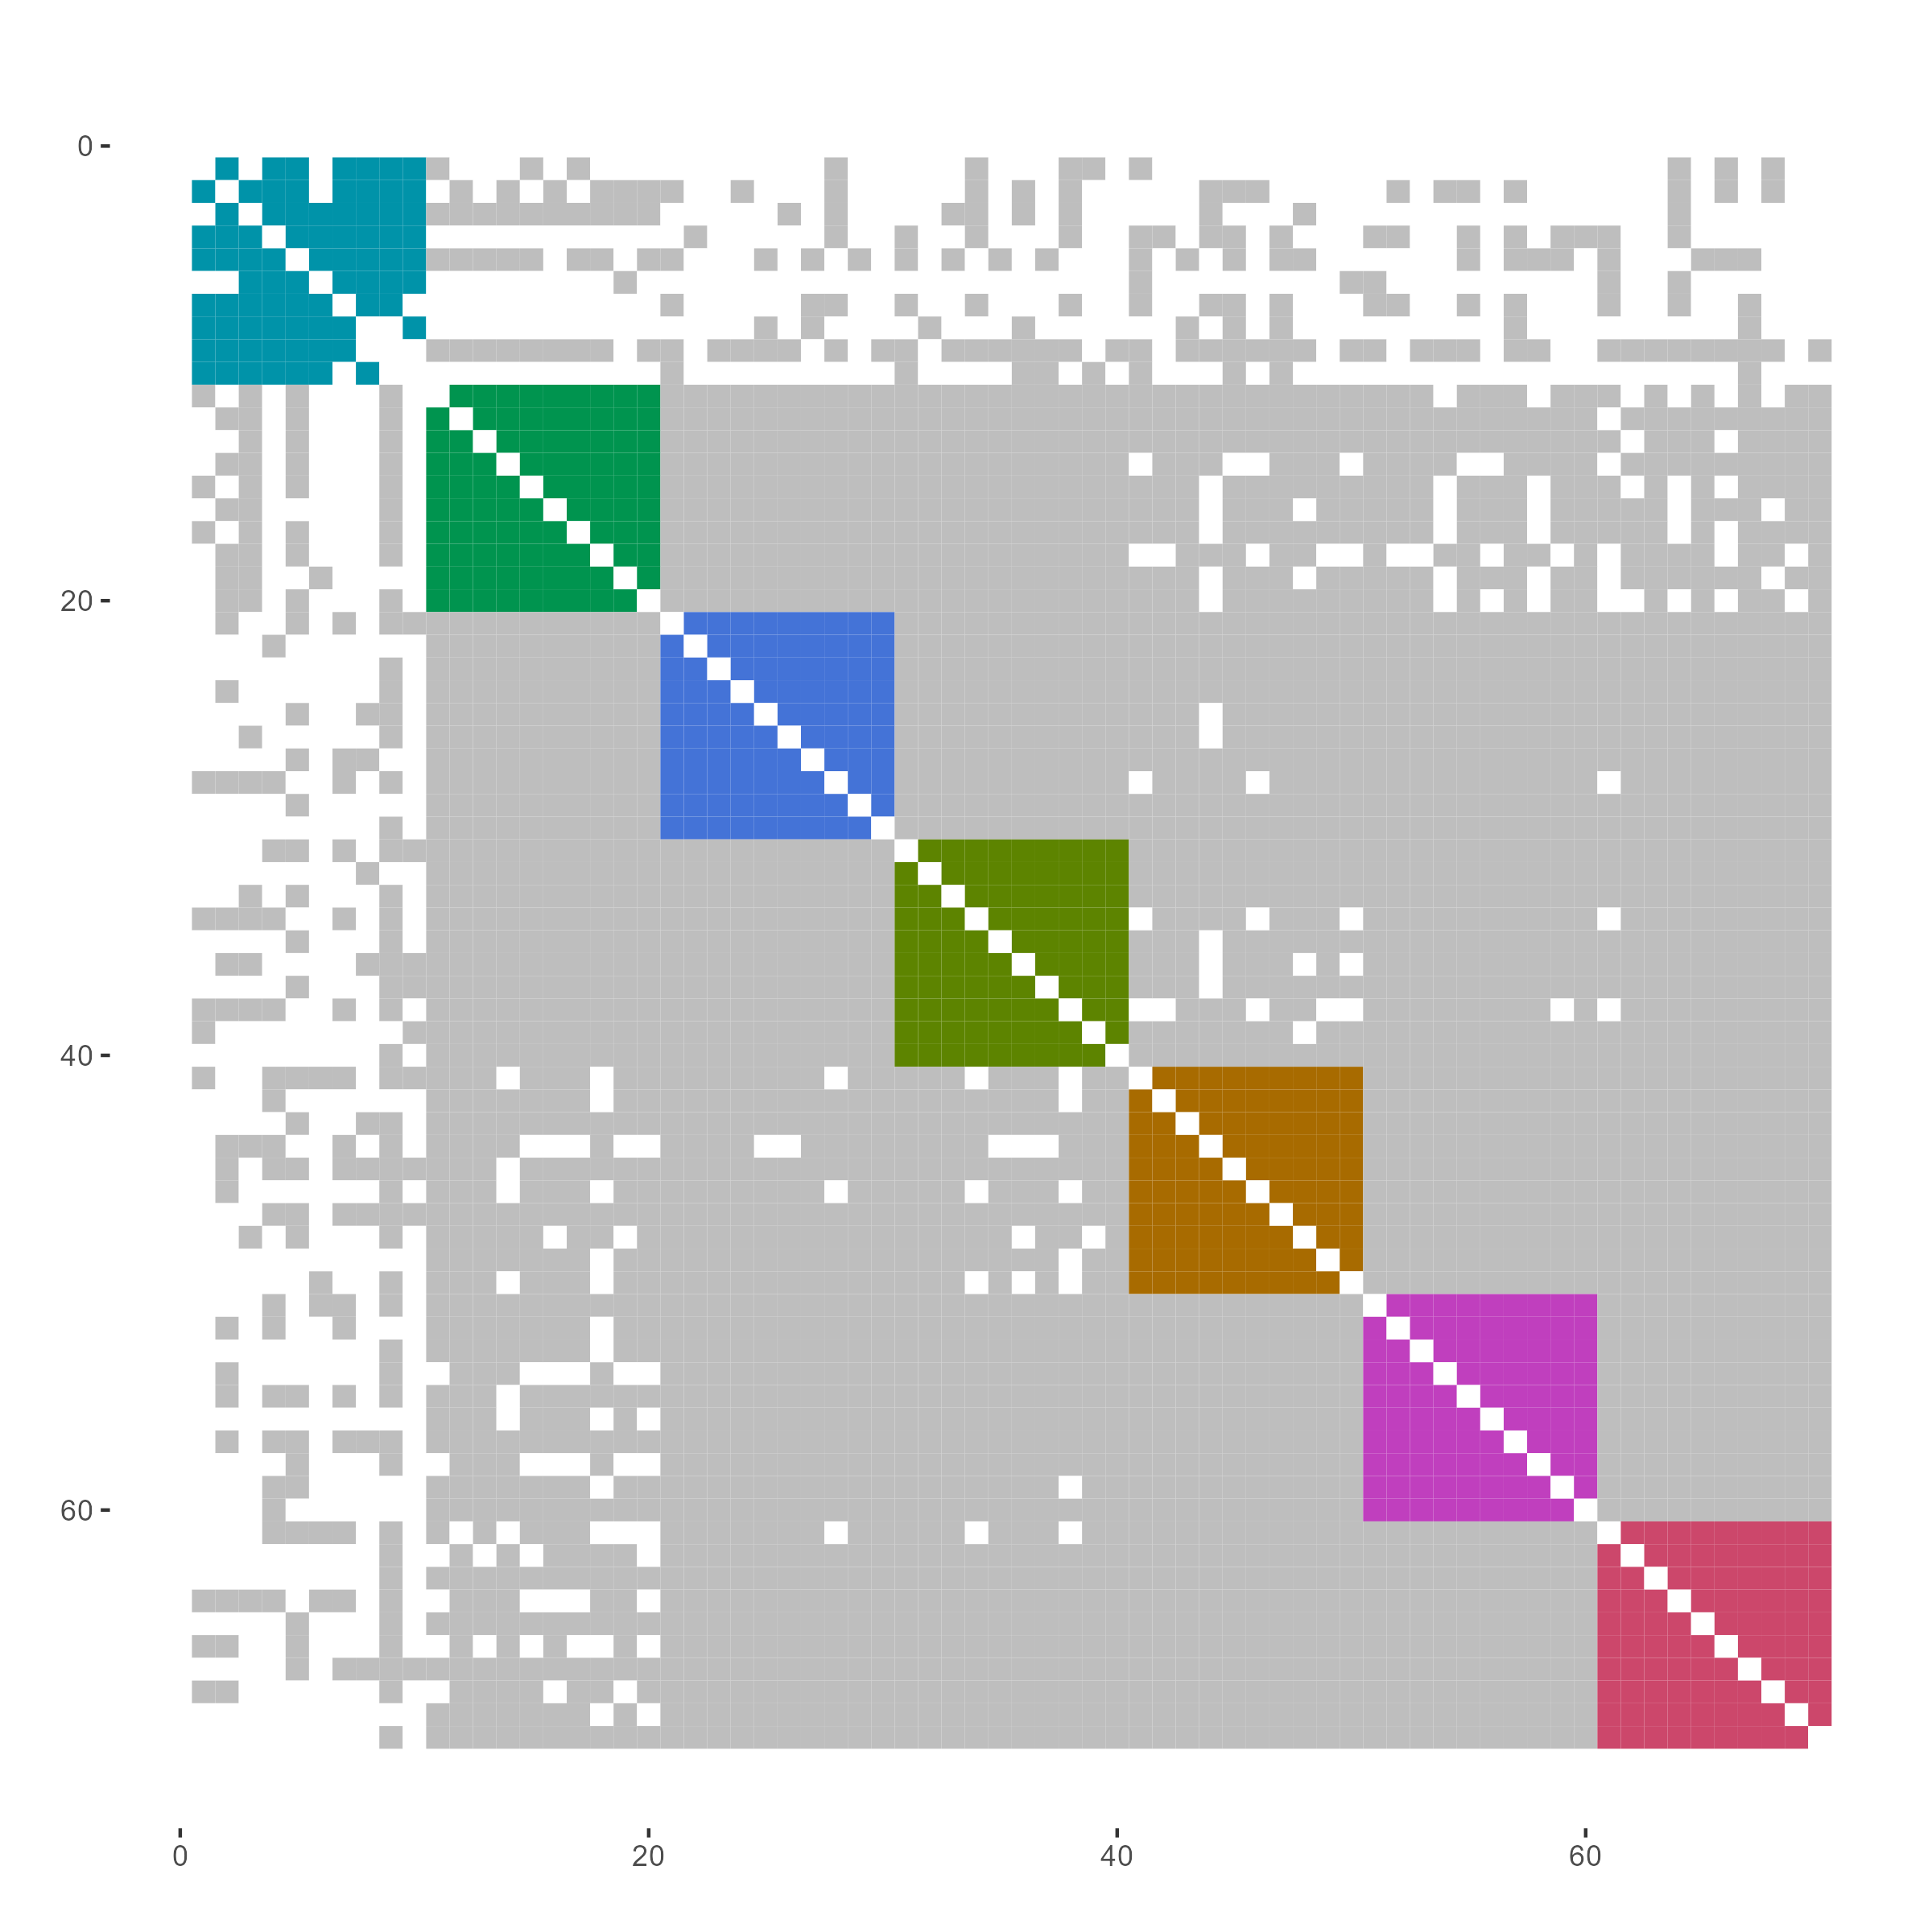
\includegraphics[scale = 0.14]{images/colored-adj_mat_mglasso_genot3_order_omic.png}
\caption{$\lambda_2$ = 3.26}
\end{subfigure}
\begin{subfigure}{0.3\linewidth}
\centering
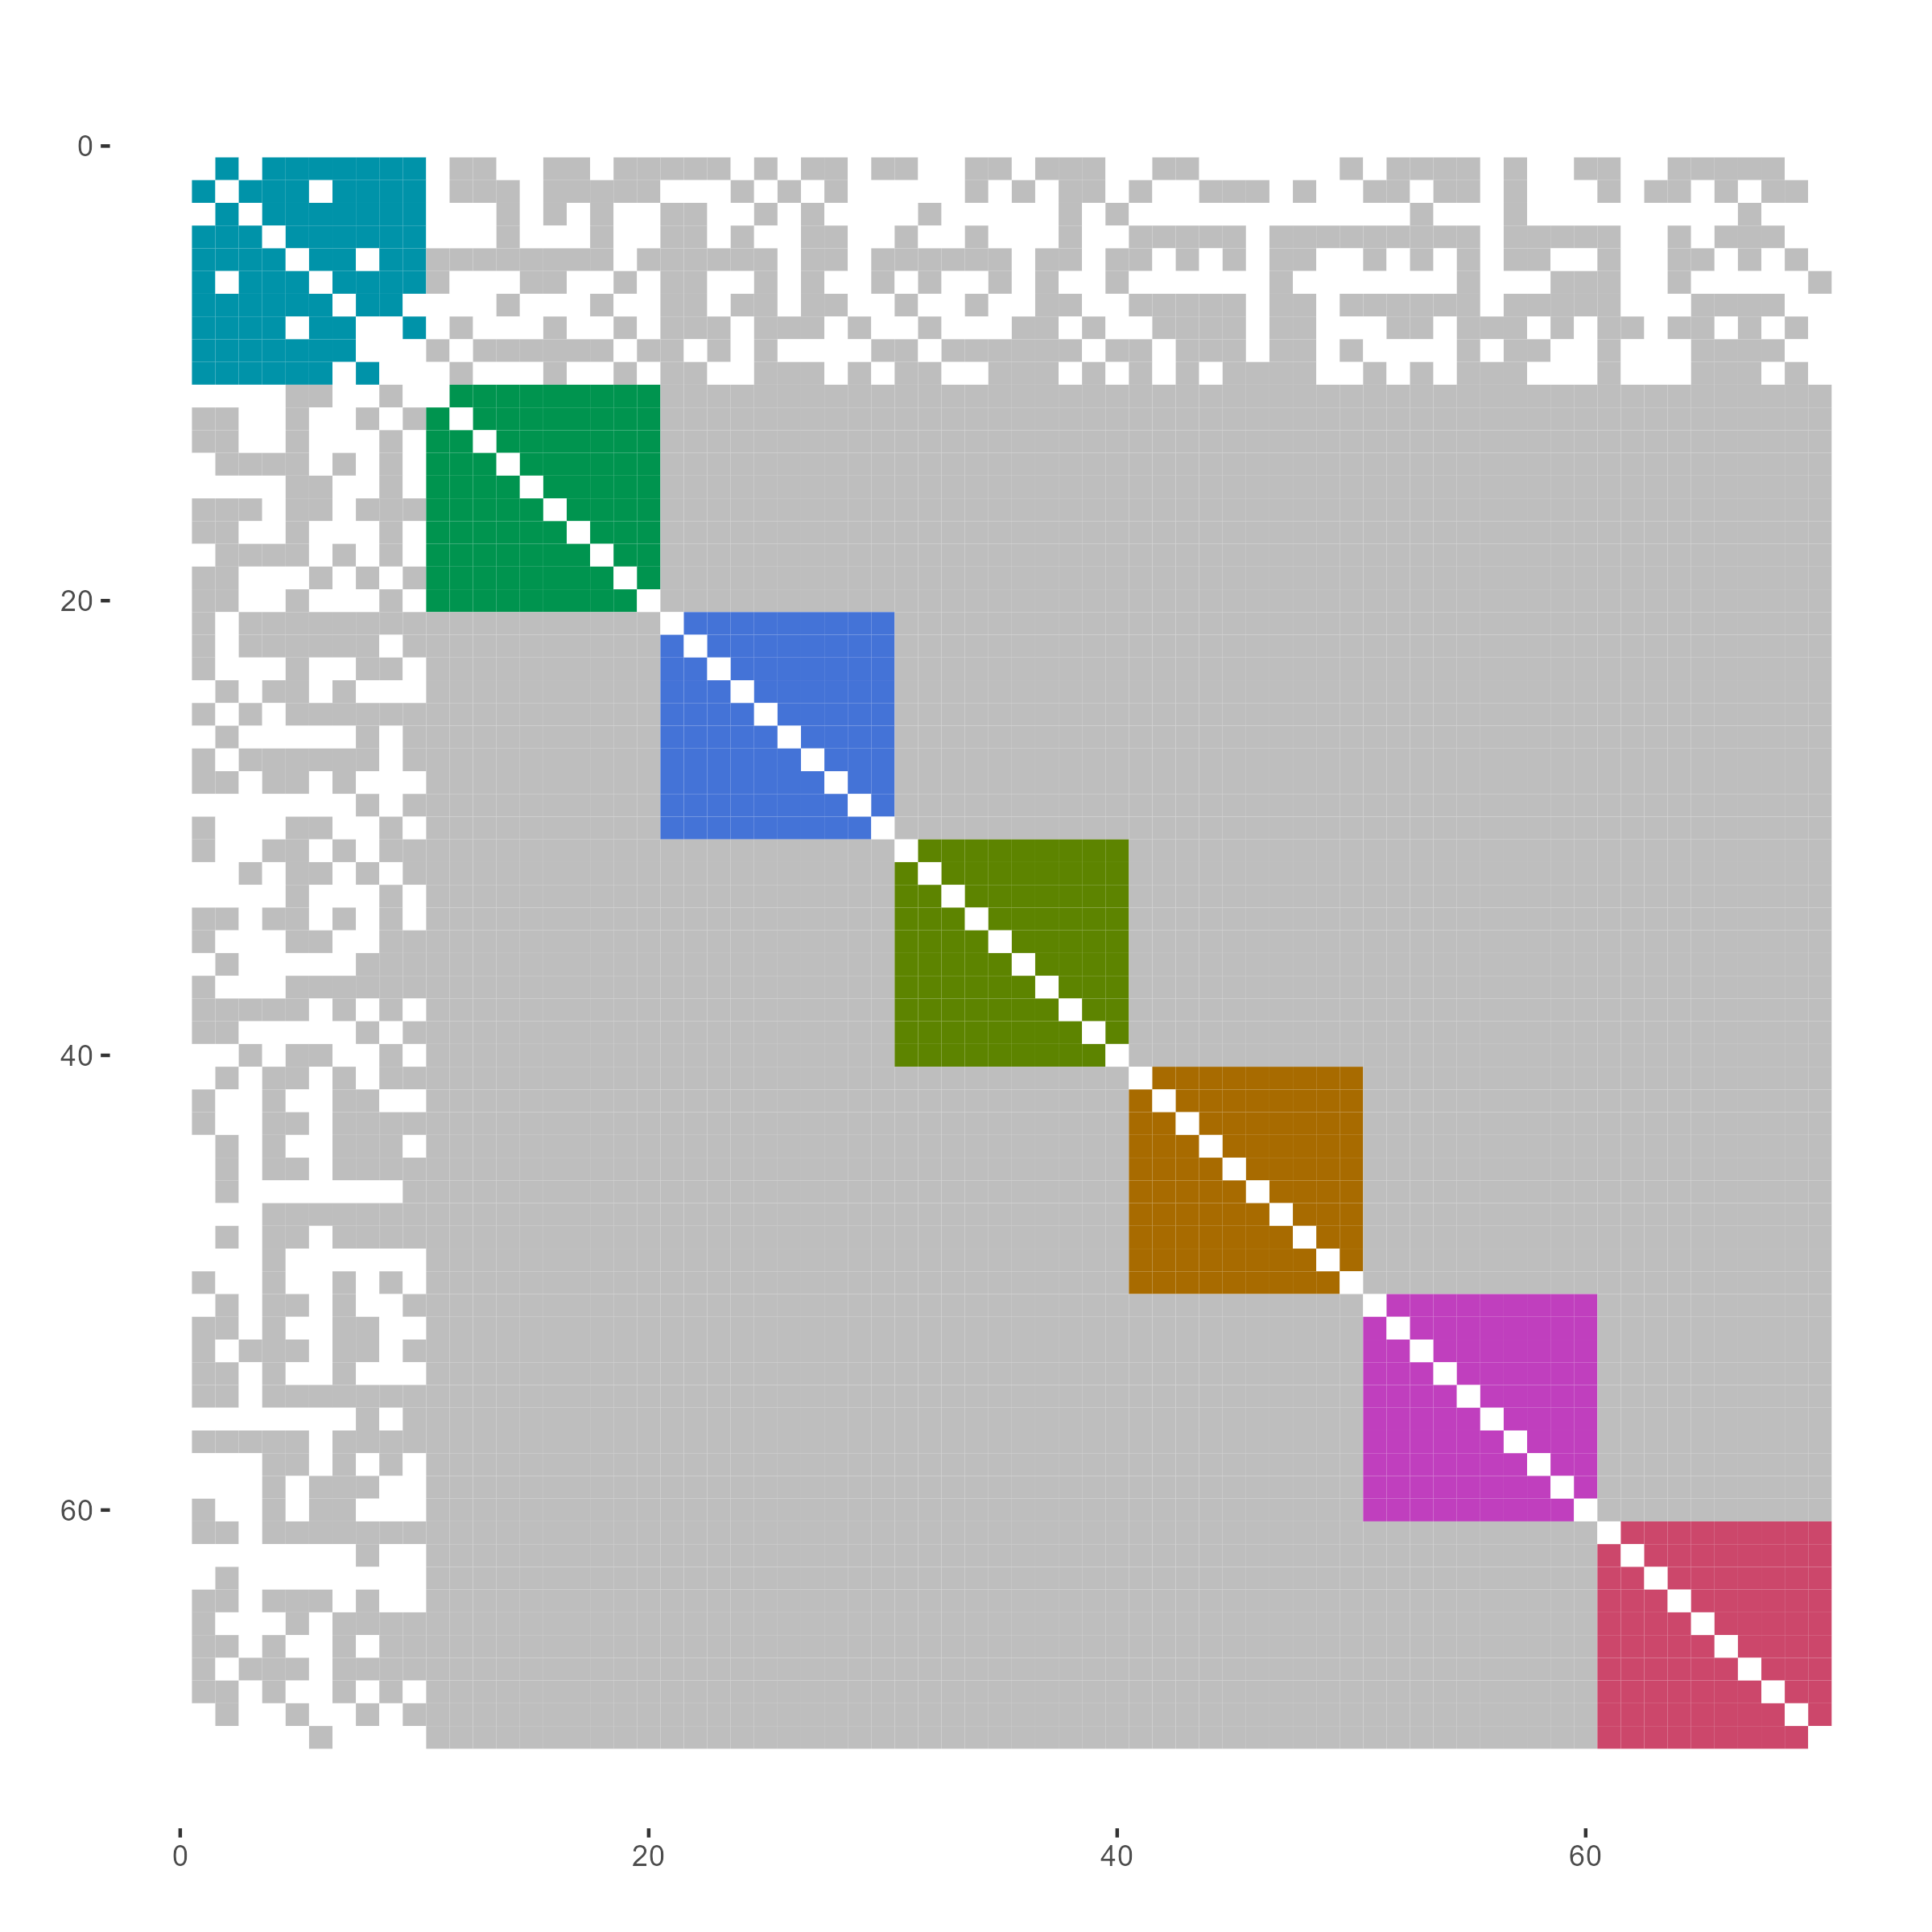
\includegraphics[scale = 0.14]{images/colored-adj_mat_mglasso_genot4_order_omic.png}
\caption{$\lambda_2$ = 4.89}
\end{subfigure}
\hfill
\begin{subfigure}{0.3\linewidth}
\centering
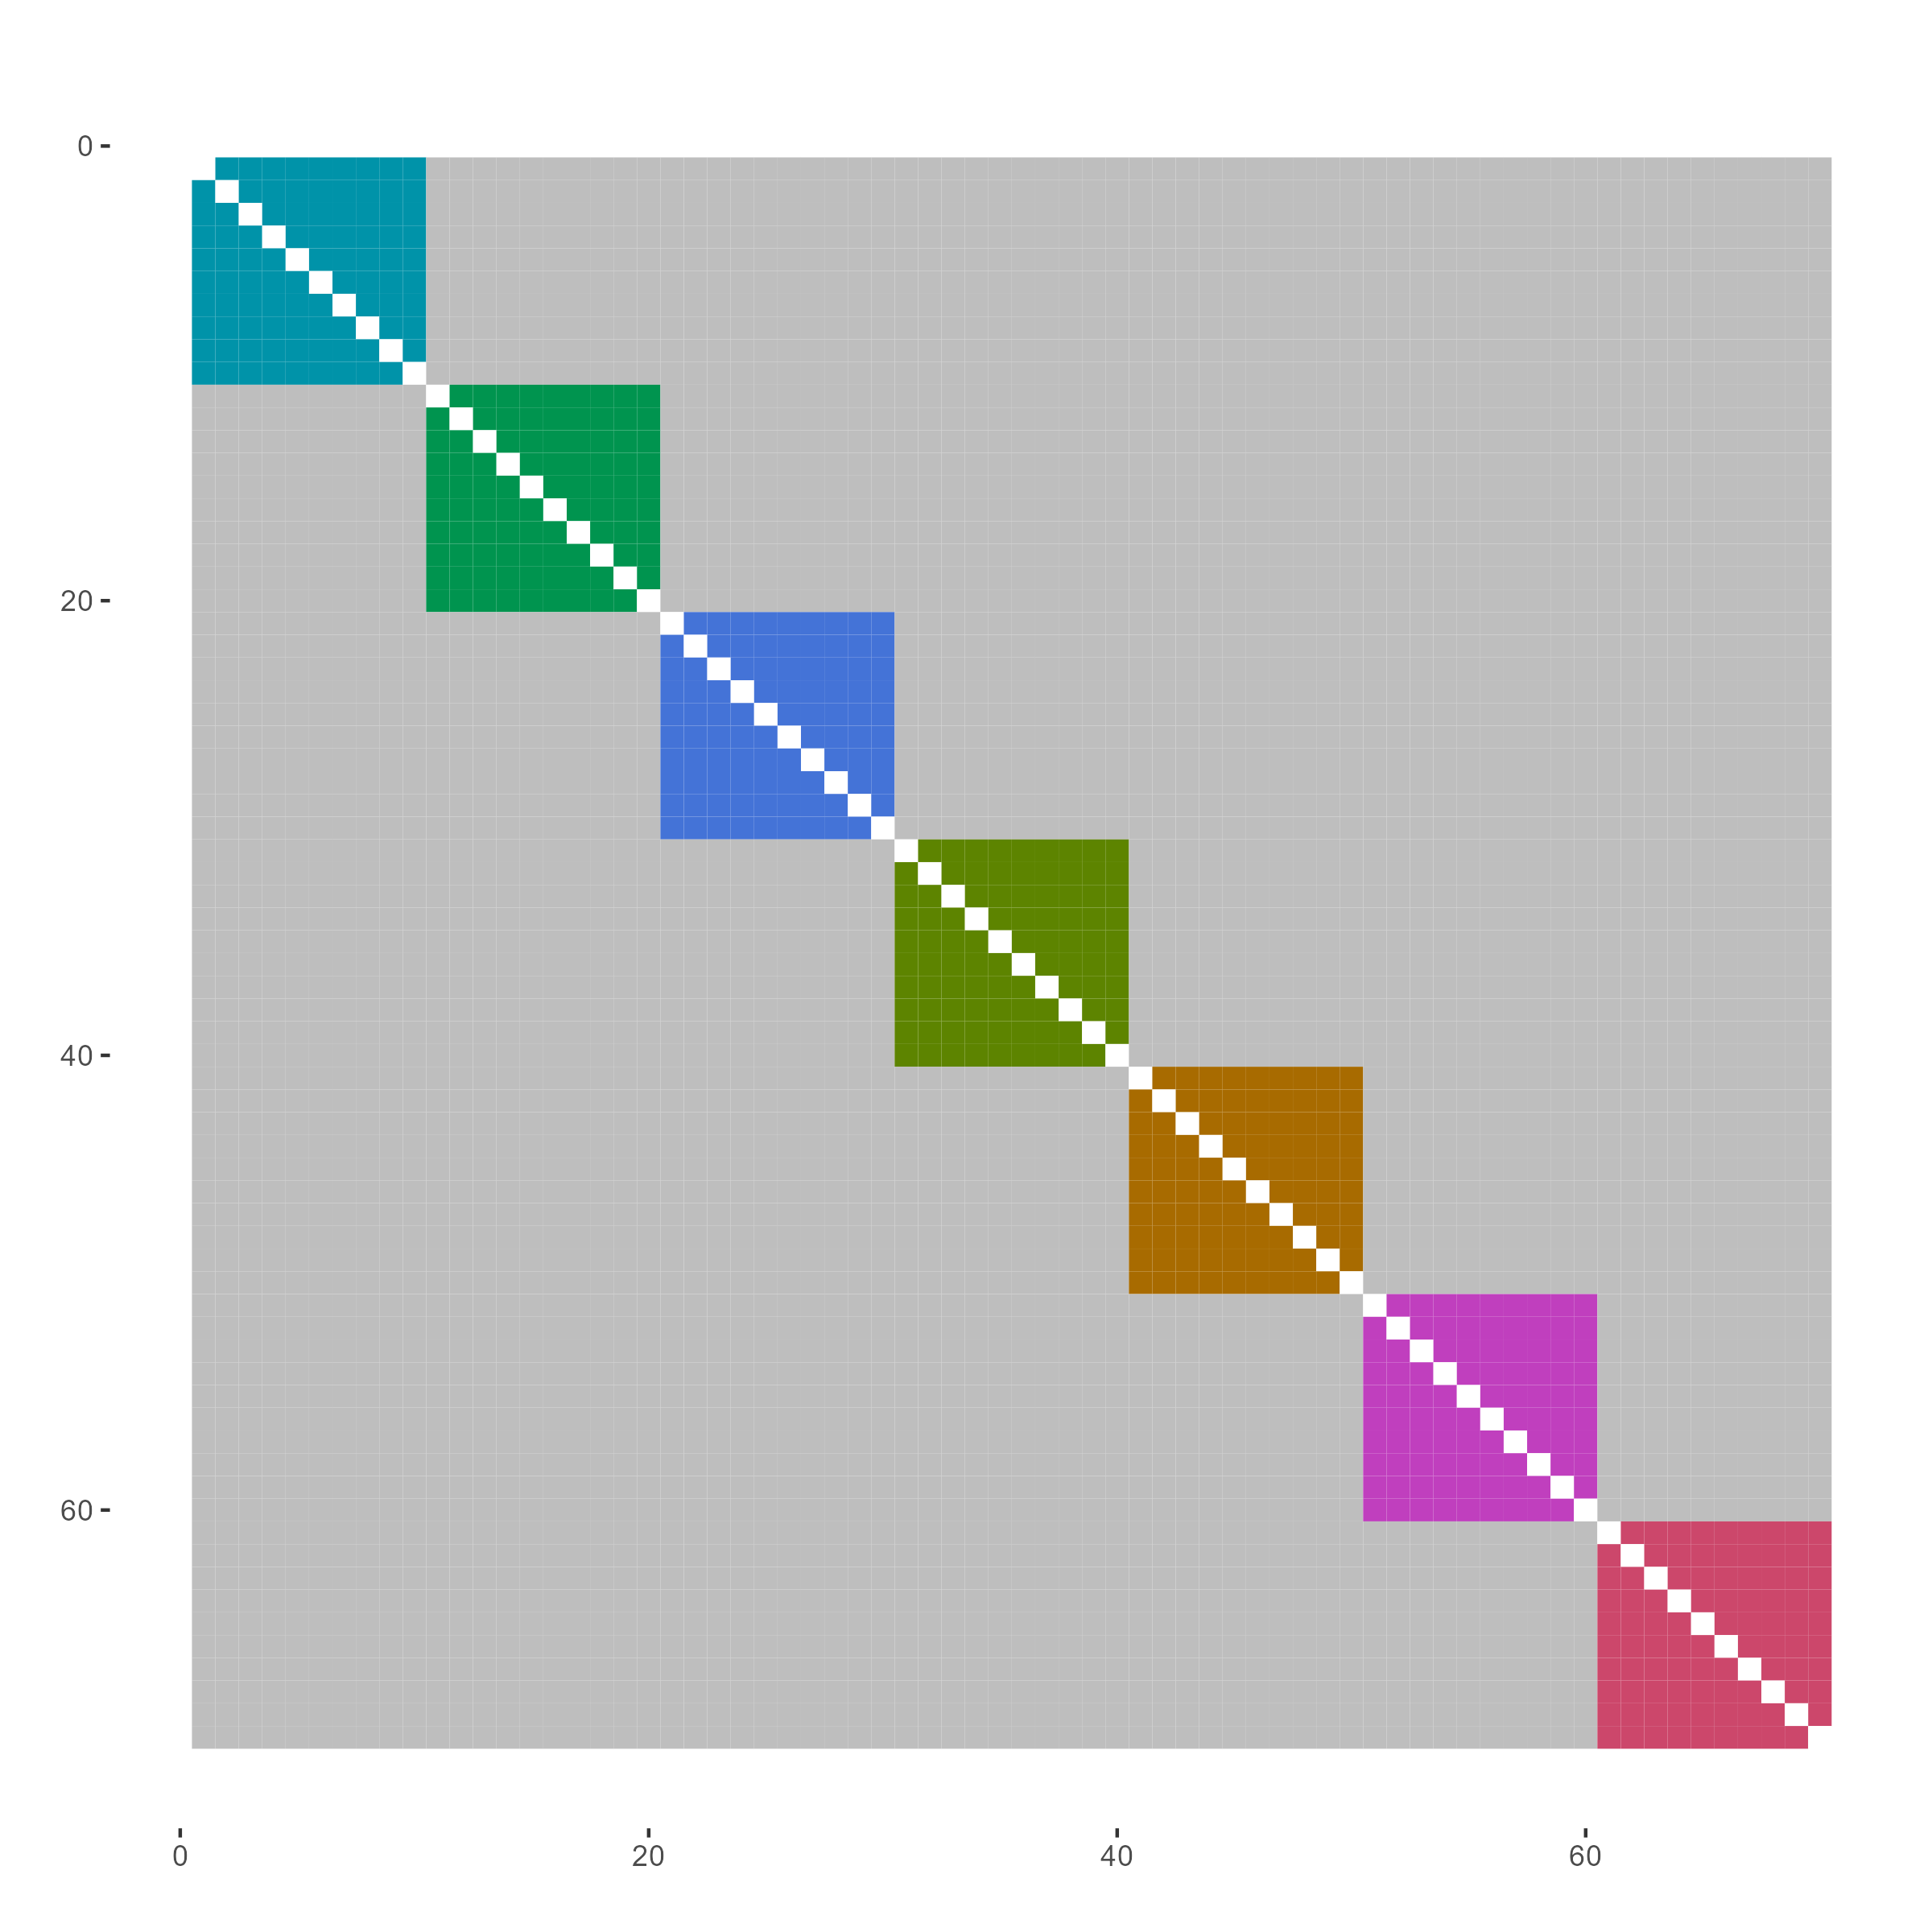
\includegraphics[scale = 0.14]{images/colored-adj_mat_mglasso_genot20_order_omic.png}
\caption{$\lambda_2$ = 30.94}
\end{subfigure}
%\caption{A figure with 6 subfigures arranged in two rows.}
\end{figure}
\end{frame}



\subsection{Discussion}


\section{Perspectives}
\begin{frame}{}
\begin{center}
\Huge{\prune{Conclusion and Perspectives}}
\end{center}
%\begin{center}
%\begin{description}
%\item[i] A
%\item[ii] B
%\item[iii] C
%\end{description}
%\end{center}
\end{frame}

\subsection{Conclusion}
\begin{frame}{Conclusion}
\begin{block}{Mathematics}
\only<2-3>{A probabilistic model for:
\begin{itemize}
	\item Inferring multiscale networks for continuous data.
	\item Estimating simultaneously clustering partition.
\end{itemize}
Based on:
\begin{itemize}
	\item Gaussian graphical modeling via pseudo log-likelihood maximization.
	\item Convex clustering theory.
	\end{itemize}}
\end{block}

\begin{block}{Applications: Life sciences}

\begin{itemize} 
\item   Epigenetics can differentiate natural populations of poplars.
%\item Multiscale exploratory genotypes-genotypes networks on integrated multi-omics data
\end{itemize}
Through
\begin{itemize}
\item \emphase{Differential analysis} of methylation data.
\item \emphase{Gene set enrichment analysis} of selected genes.
\end{itemize}
\end{block}
\end{frame}

\subsection{Extensions}
\begin{frame}{Extensions}
\begin{block}{Convex clustering}
\begin{itemize}
\item Conditions for which one can recover a tree structure.
\item Bounds on regularization parameters.
\end{itemize}
\end{block}

\begin{block}{Network inference}
\begin{itemize}
\item Penalized maximum likelihood estimator.
\item Fitting \emphase{mixed graphical models} for heterogeneous data.
\end{itemize}
\end{block}
 
\begin{block}{Optimization}
\begin{itemize}
\item Scale to high dimensional data.
\end{itemize}
\end{block}
\end{frame}

\subsection{Contributions}
\begin{frame}{Contributions}
\begin{description}
\item[Articles] \begin{itemize}
\item[]\vspace{-0.5cm}\small
\item E. Sanou, C. Ambroise, G. Robin \textit{"Inference of Multiscale Gaussian Graphical Model."} \emphase{Computo} (2023)\vspace{0.2cm}
\item  M. Sow et al. \textit{"Epigenetic Variation in Tree Evolution: a case study in black poplar (Populus nigra)."}  bioRxiv 2023.07.16.549253. \emphase{Submitted to New Phytologist} (2023).
\end{itemize}\vspace{0.5cm}
\item[R packages] \begin{itemize}
\item[]\vspace{-0.5cm}\normalsize
\item E. Sanou \textit{"\emphase{mglasso}: Multiscale Graphical Lasso."}: CRAN, 2022 \url{https://CRAN.R-project.org/package=mglasso}.\vspace{0.2cm}
\end{itemize}
\end{description}  
\end{frame}

\subsection{}
\begin{frame}{}
\centering
Thank you for your attention.
\end{frame}

									
										\appendix
										\backupbegin
										\begin{frame}[allowframebreaks]
											\bibliographystyle{apalike}
											{\tiny
												\bibliography{biblio}}
											\frametitle{References}
											%\bibliography{cellcite}
										\end{frame}
										
										\begin{frame}{sparse PCA for gene selection (1)}
											\centering
											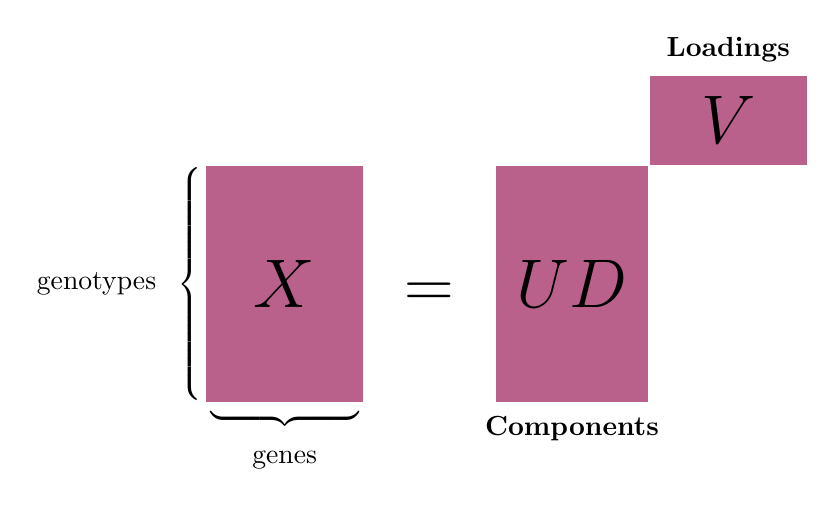
\begin{tikzpicture}[absolute, node distance=+0cm, scale=0.9]
												% Original Data Matrix
												\node[big=2x3, left delimiter=\{, below delimiter=\}, tighter delimiters] (X) {$X$};
												\node[below=0.5cm] at (X.south) {genes};
												\node[left=0.5cm of X] {genotypes};
												
												% Equal sign
												\node[big'=0x0, base right=of X] (eq) {${}={}$};
												
												% Loadings Matrix
												\node[big=1x3, base right=of eq, tighter delimiters] (A) {$UD$};
												\node[below=0.05cm] at (A.south) {\textbf{Components}};
												
												% Principal Components Matrix
												\node[big=2x1, anchor=south west, at=(A.north east), tighter delimiters] (B) {$V$};
												\node[above=0.05cm] at (B.north) {\textbf{Loadings}};
												
											\end{tikzpicture}
											\begin{block}{PCA: Dimension reduction}
												\begin{itemize}
													\item Via SVD of the data matrix $\mathbf X = \mathbf U \mathbf D \mathbf V^\top$ 
													\item PCs are linear combinations of all the genes
												\end{itemize}
											\end{block}
										\end{frame}
										
										\begin{frame}{sparse PCA for gene selection (2)}
											\begin{block}{PCA as a low rank matrix approximation problem}
												\only<1>{\begin{itemize}
														\item Sum of rank $1$ matrices 
														\begin{align*} 
															\mathbf X &= \mathbf U(\mathbf D_1 + \mathbf D_2 + \hdots + \mathbf D_p) \mathbf V^\top \\ 
															&= d_1 \mathbf u_1 \mathbf v_1^\top + \dots +  d_p \mathbf u_p \mathbf v_p^\top
														\end{align*}
														\item  PCA seeks the best rank $1$ approximation of $\mathbf X:$ $$\min{\mathbf{a}, \mathbf{v}} \left \| \mathbf X - \mathbf{{a}  {v}^\top} \right \|_F^2$$ for the first pair of singular vectors $\mathbf a_1 = d_1 \mathbf u_1$ and $\mathbf v_1.$ 
														\item Then find $(\mathbf a_2, \mathbf v_2)$ as the best rank $1$ approximation of $\mathbf X - \mathbf a_1 \mathbf v_1^\top$
												\end{itemize}}
											\end{block}
											\onslide<2->
											\begin{block}{sparse PCA}
												$$\min{\mathbf{a}, \mathbf{v}} \left \| \mathbf X - \mathbf{{a}  {v}^\top} \right \|_F^2 + \lambda \left \| \mathbf{ v} \right \|_1 $$ subject to $\|\mathbf{{a}}\|_2 = 1.$
											\end{block}
											
											\begin{block}{Procedure}
												\begin{itemize}
													\item Apply sparse PCA and select $15$ top-genes for the $3$ PCs using \texttt{mixomics}
													\item Merge genes lists for all the omics and remove duplicates: $151$ genes 
												\end{itemize}
											\end{block}
										\end{frame}									

										
										\begin{frame}{}
											\begin{center}
												\Huge{\prune{Application on microbial abundance data}}
											\end{center}
											% 	\begin{center}
												% 		\begin{description}
													% 			\item[i] A
													% 			\item[ii] B
													% 			\item[iii] C
													% 		\end{description}
												% 	\end{center}
										\end{frame}
										
										\begin{frame}{Microbial abundance data}
											Microbial abundance data collected as part of the American Gut project \citep{mcdonald2018american}.
											\begin{itemize}
												\item $n = 289$ samples via an abundance table for $p = 127$ types of microbes (operational taxonomic units).
												\begin{table}[ht]
													\centering
													\begin{tabular}{cccc}
														OTU 1 & OTU 2 & \dots & OTU 127\\ 
														\hline
														0 & 7 & \dots & 0 \\ 
														0 & 43 & \dots & 4 \\ 
														8 & 0 & \dots & 2 \\ 
														0 & 0 & \dots & 0 \\ 
														\dots & \dots & \dots & \dots \\ 
														0 & 0 & \dots & 346 \\ 
													\end{tabular}
													\caption{Matrix of OTUs}
												\end{table}
												\item Data transformed with the centered log-ratio (clr, \cite{aitchison1982statistical}). 
											\end{itemize}
										\end{frame}
										
										\begin{frame}{OTUs clustering path}
											%merge
											\begin{figure}[!ht]
												\centering
												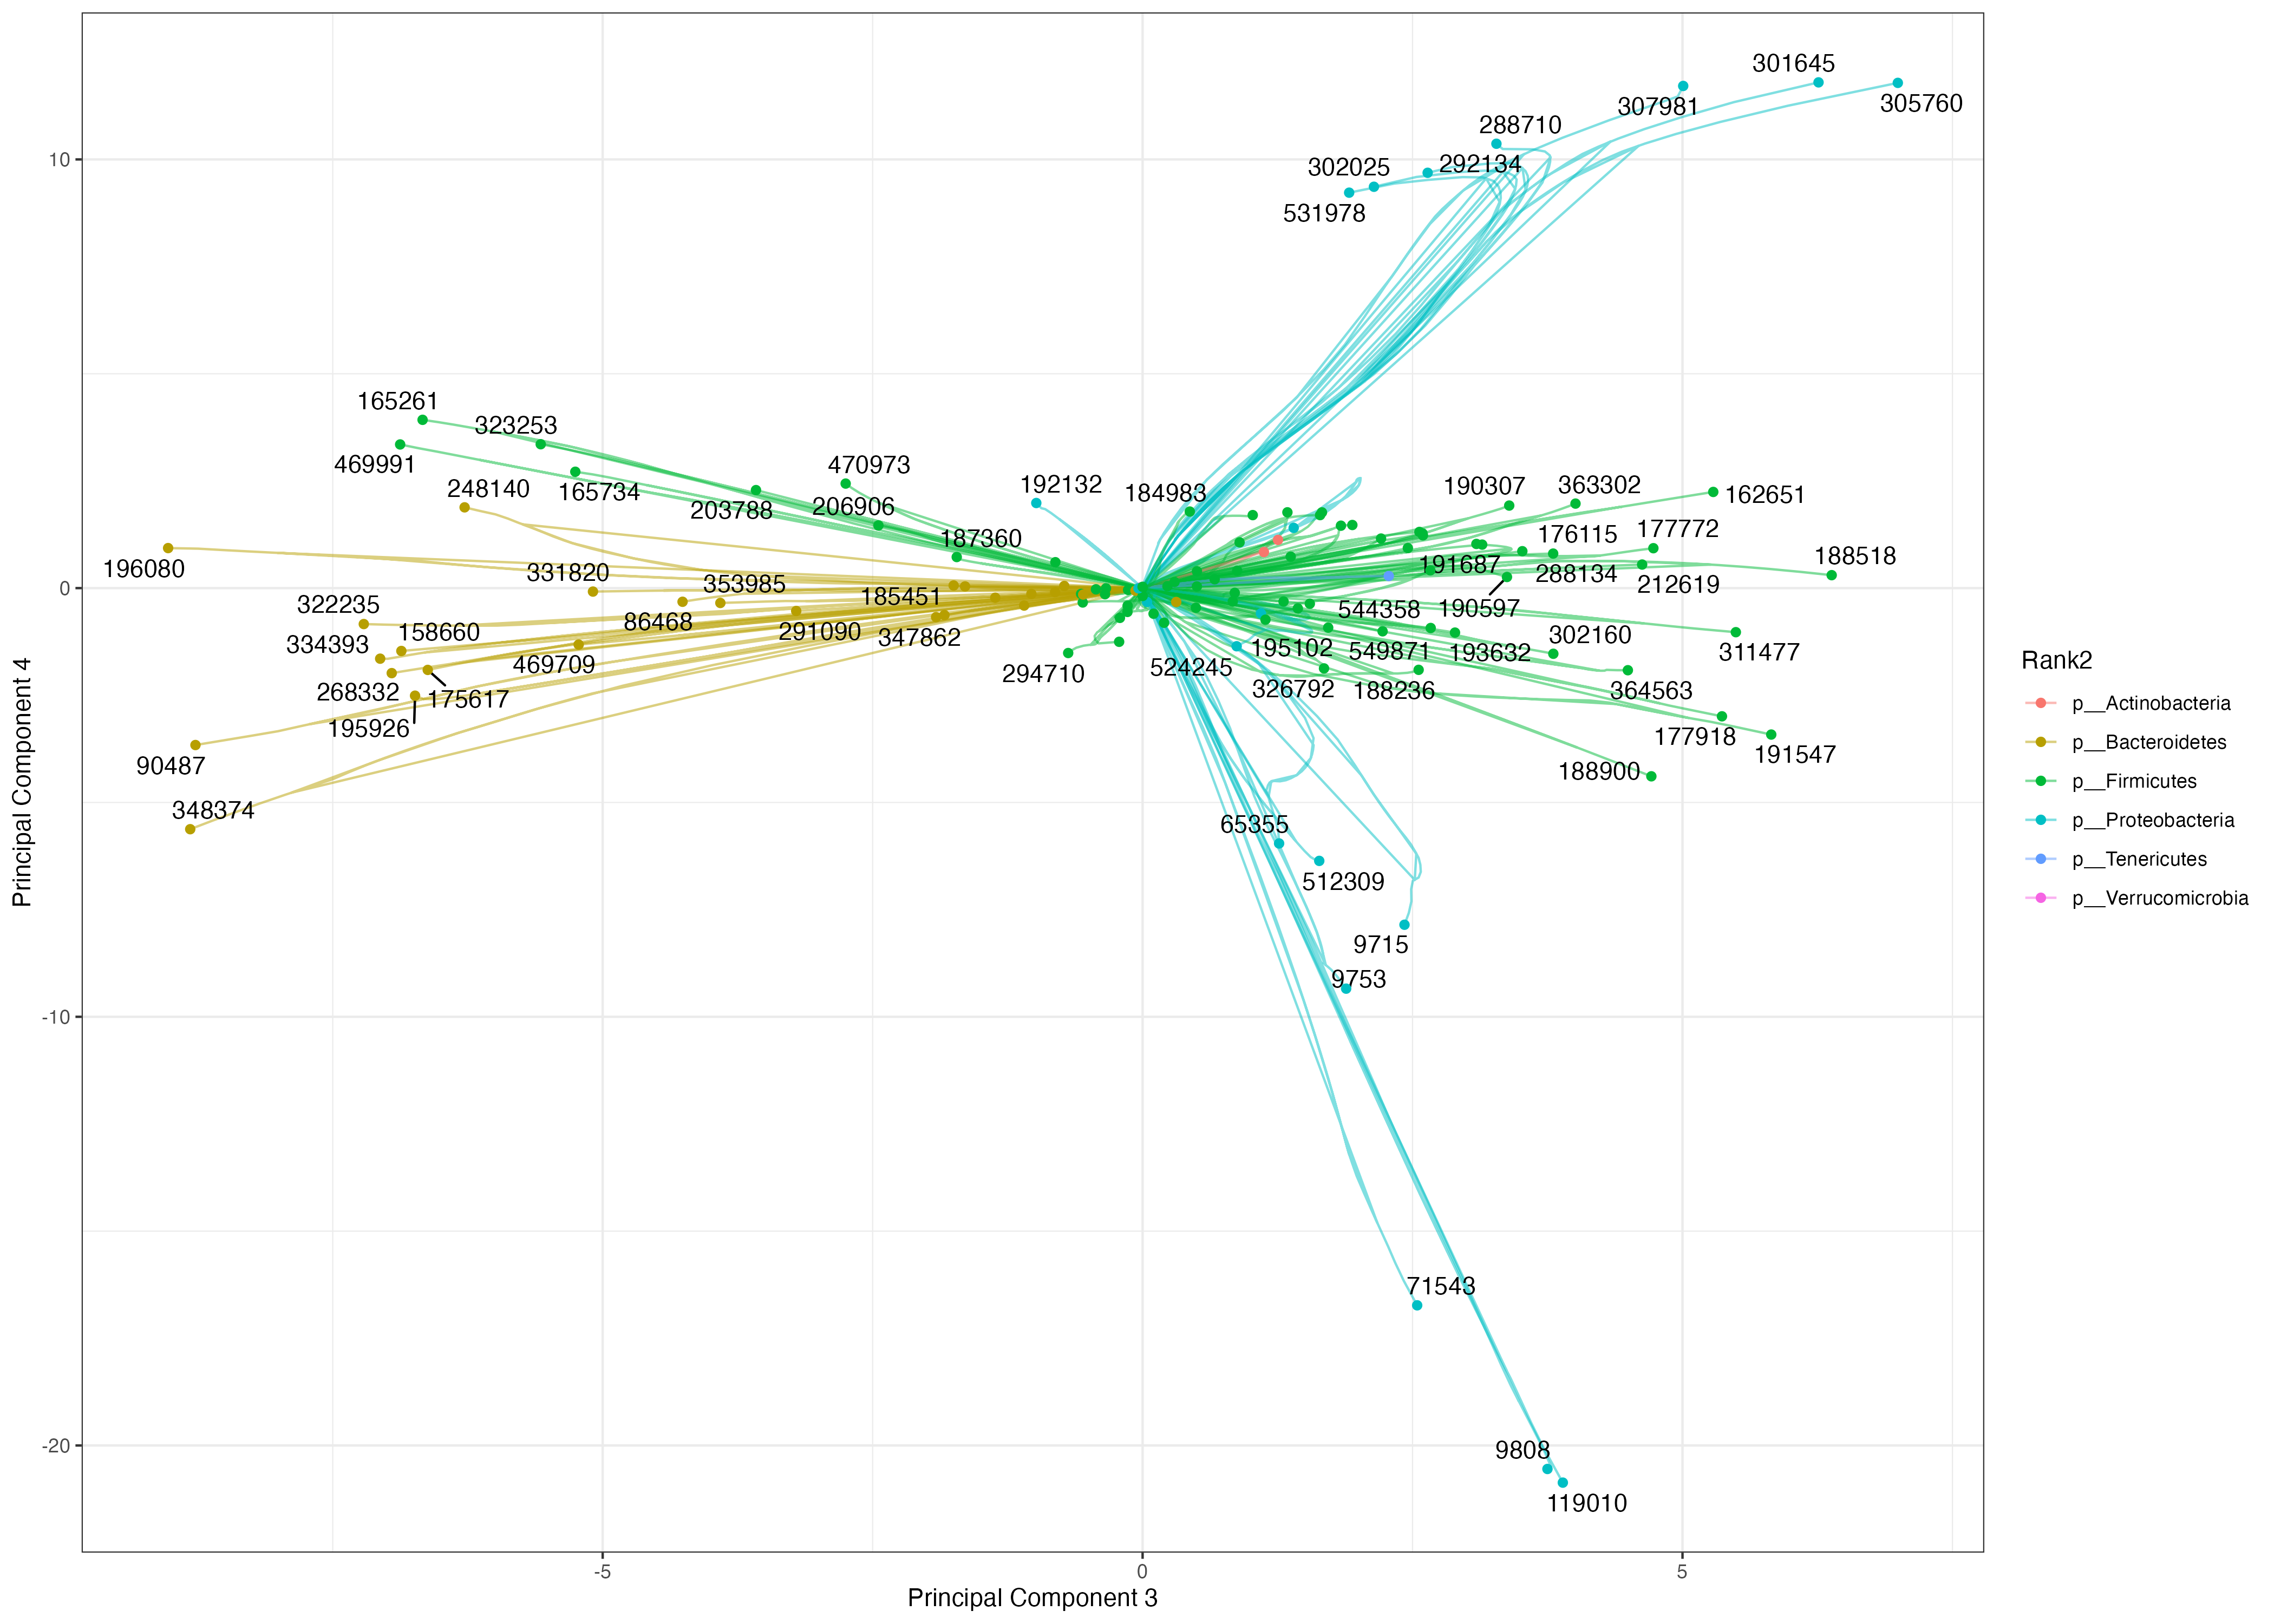
\includegraphics[scale=0.3]{images/clusterpath-gut-data.png}
												\caption{Clustering path of MGLasso solutions on human microbiome data composed of $127$ operational taxonomic units. OTUs are colored according to their phylum classification. The path displays abrupt merges. The pure cluster on the graph's left side (down) corresponds to the phylum Bacteroidetes.}
												\label{fig-clusterpath}
											\end{figure}
										\end{frame}
										
										\begin{frame}{OTUs networks} 
											
											\only<1>{
												\begin{figure}[H]
													\centering
													\subfloat[$\lambda_2 = 0$]{\label{fig:graph-path-gut-127clusters}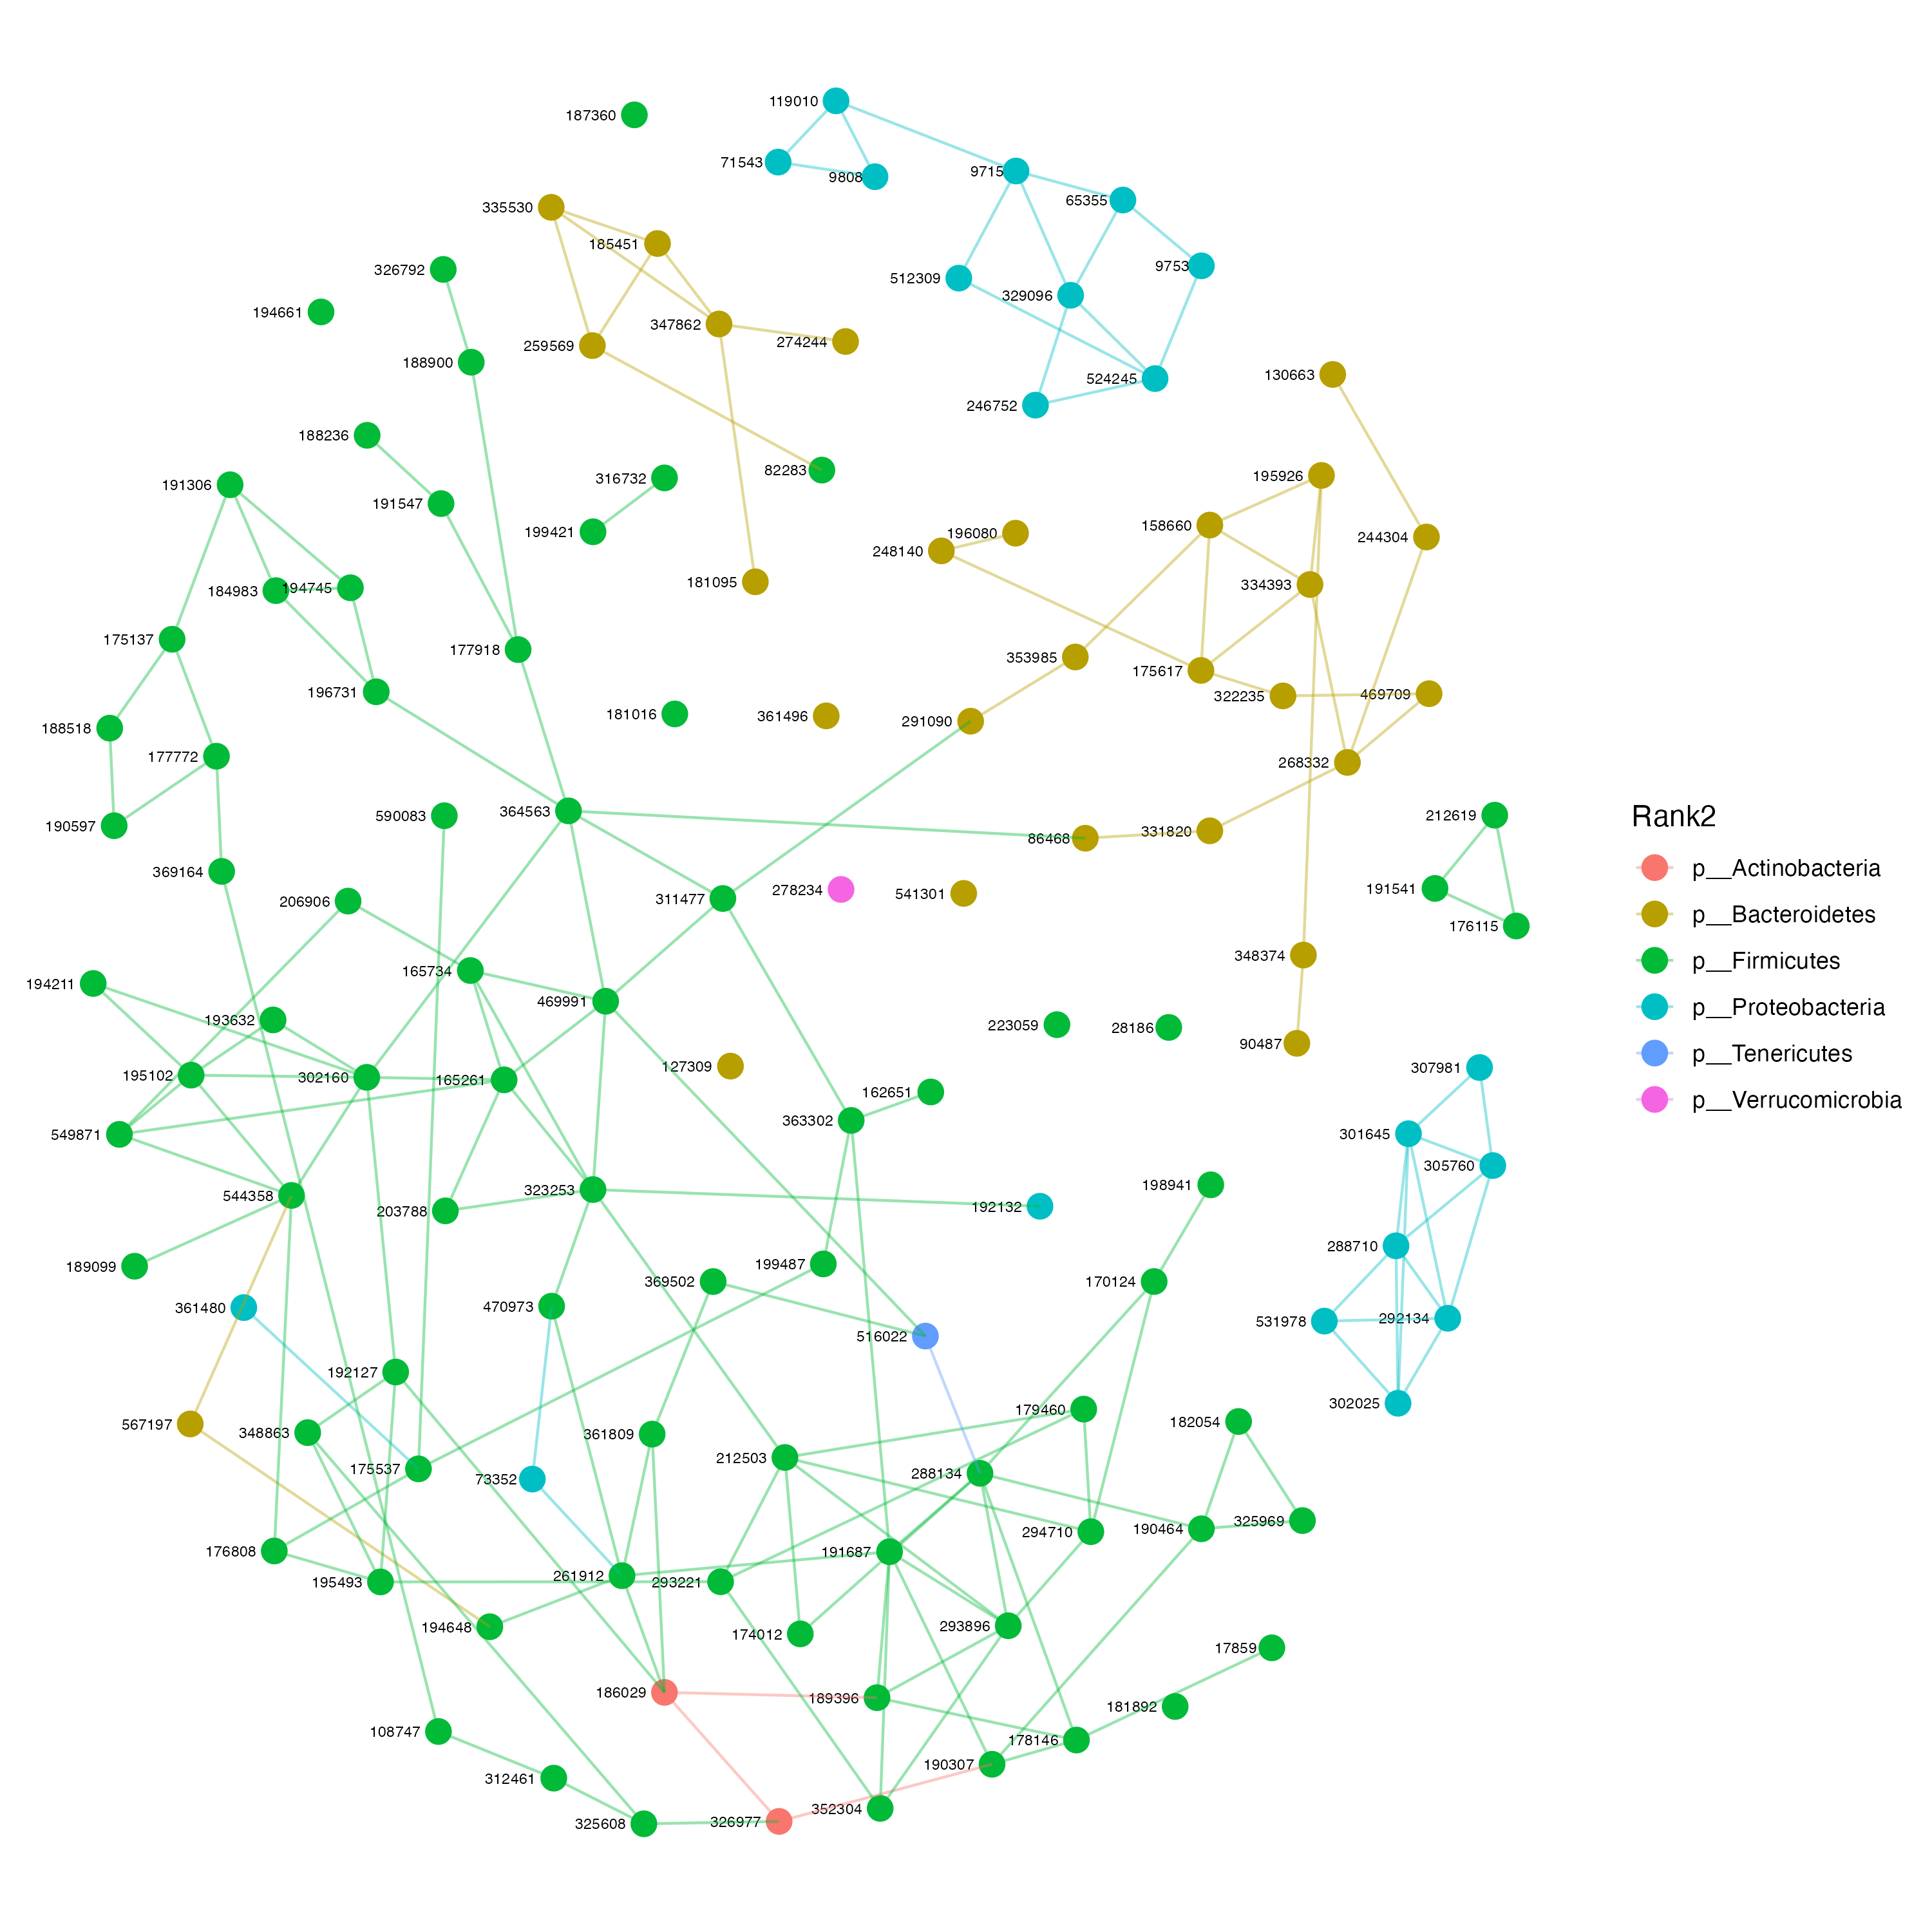
\includegraphics[height=4.7cm]{images/graph-path-gut-127clusters-175edges.png}}
												\end{figure}
											}
											\only<2>{
												\begin{figure}[H]
													\centering
													\subfloat[$63$ clusters]{\label{fig:graph-path-gut-63clusters} \includegraphics[height=4.7cm]{images/graph-path-gut-63clusters-548edges.png}}
													\subfloat[$31$ clusters]{\label{fig:graph-path-gut-31clusters}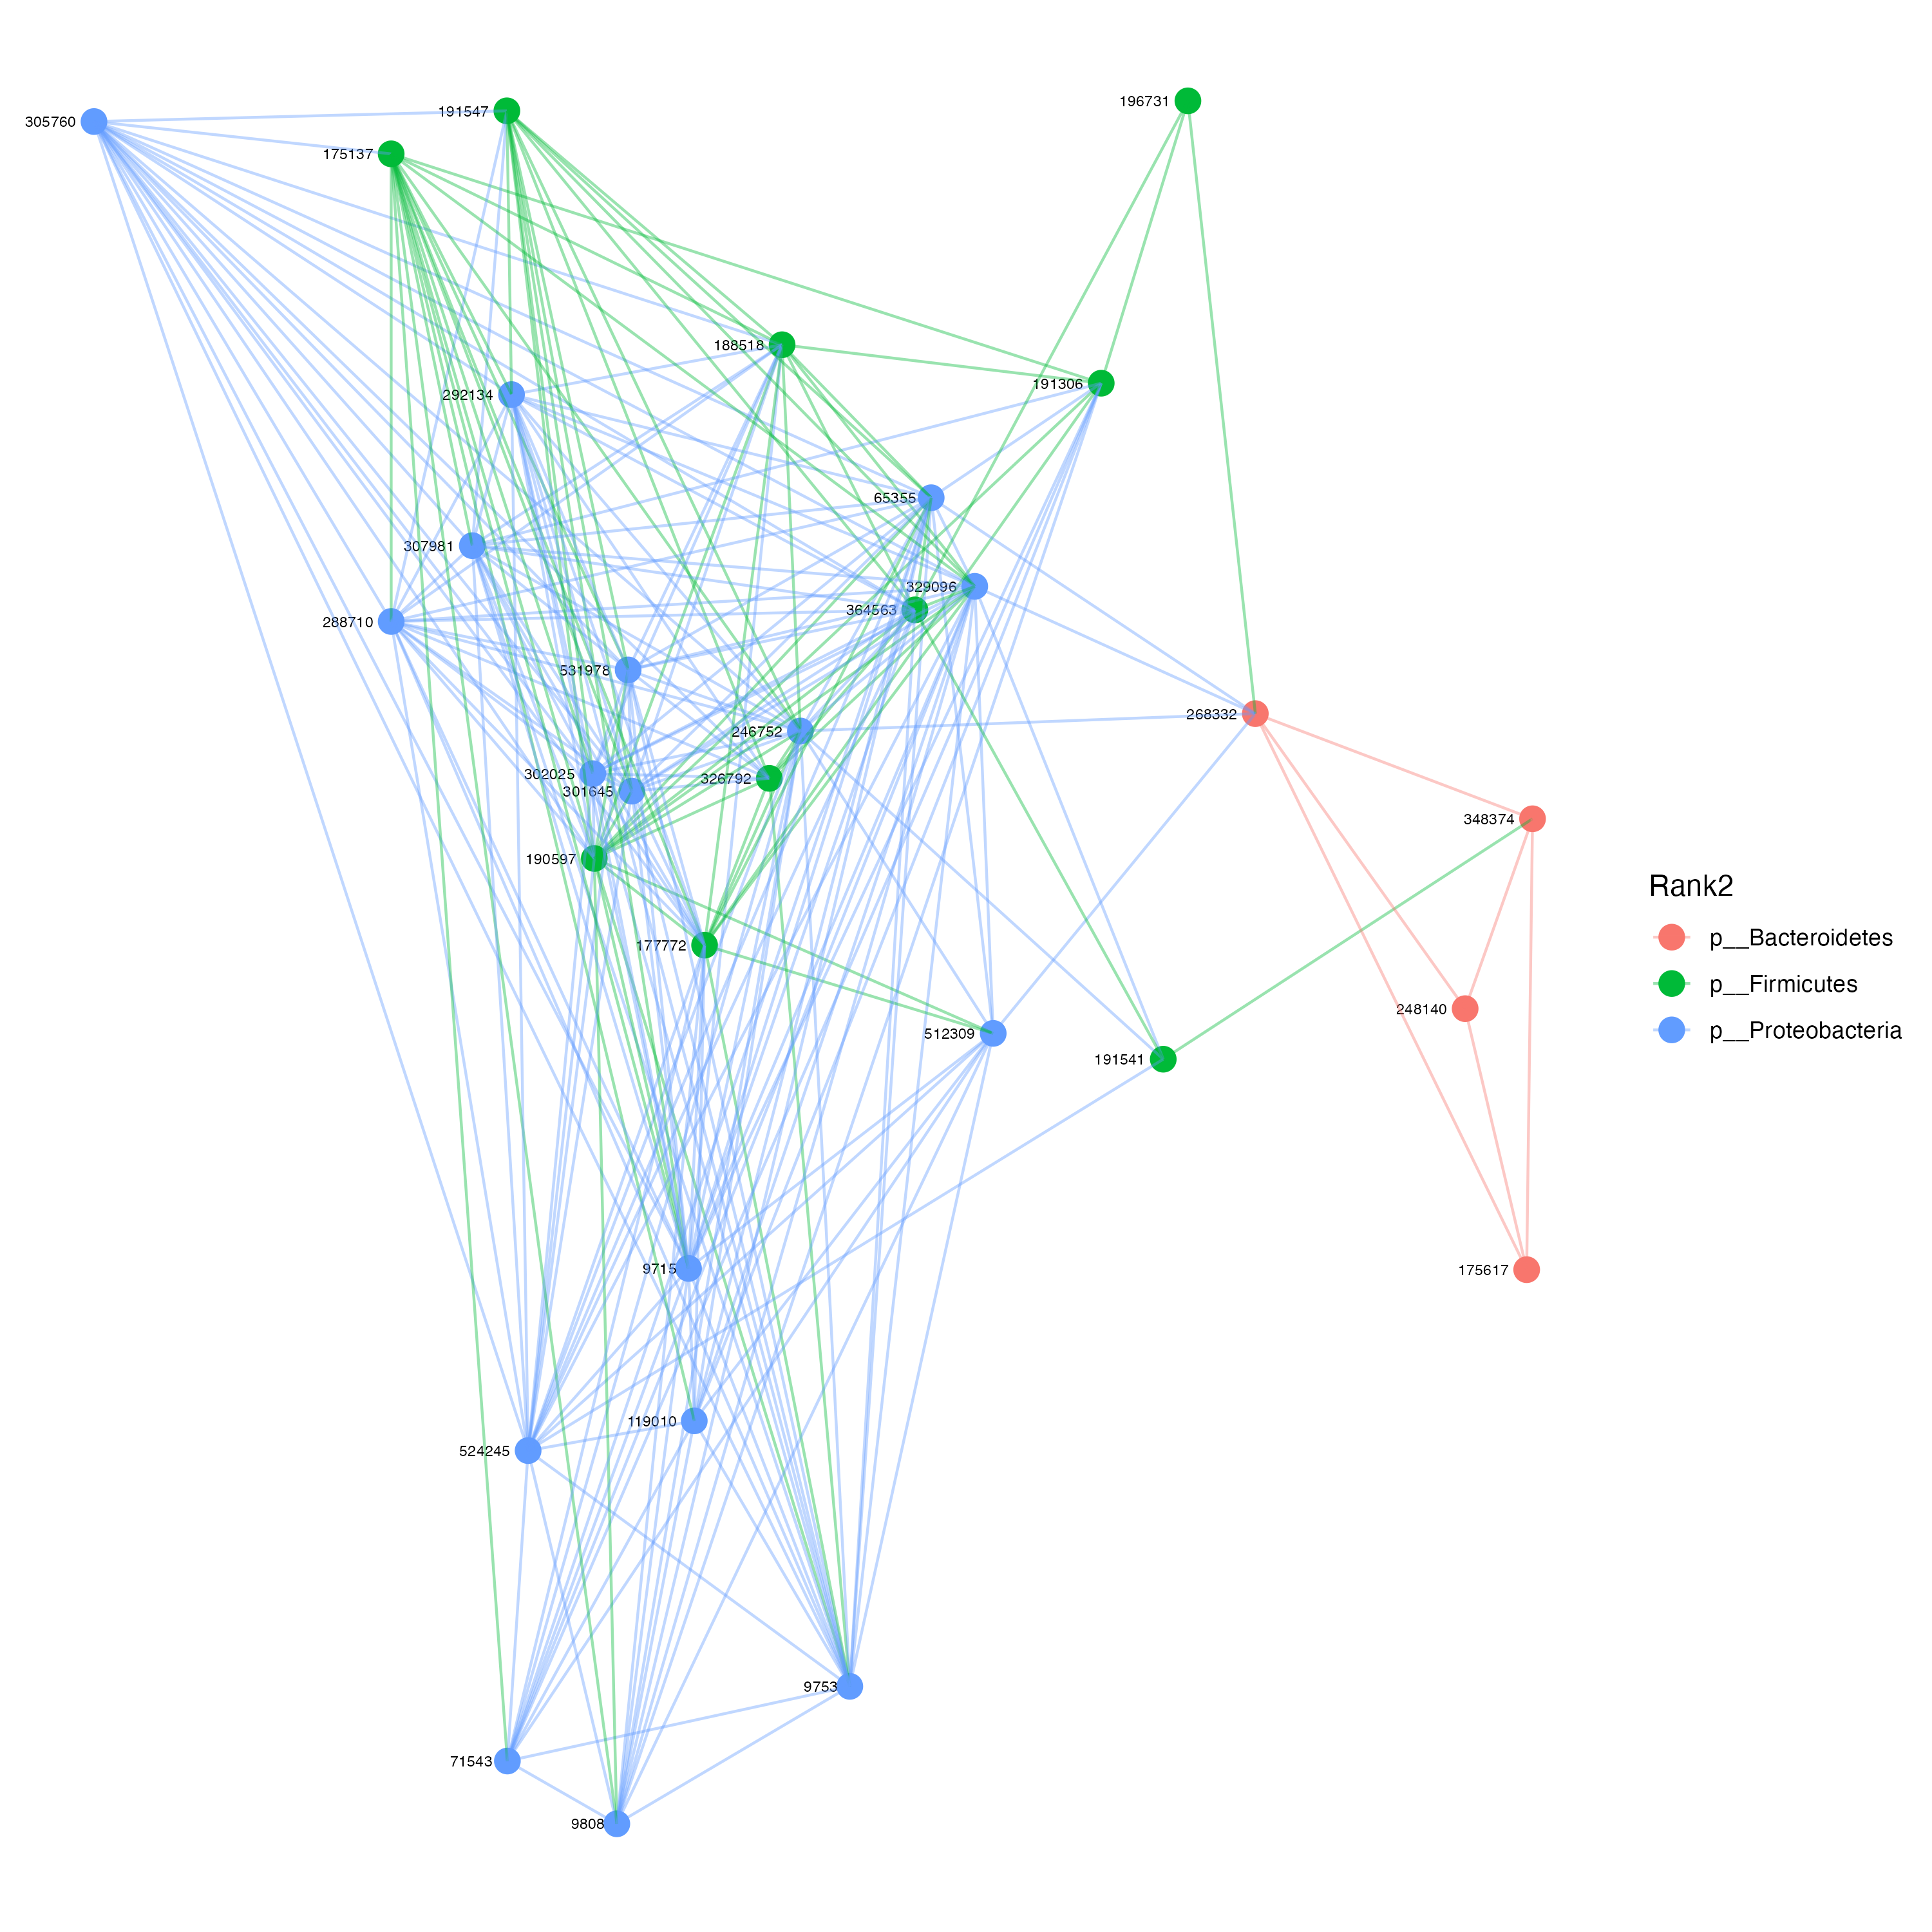
\includegraphics[height=4.7cm]{images/graph-path-gut-31clusters-240edges.png}}
												\end{figure}
											}
											\only<3>{
												\begin{figure}
													\centering
													\subfloat[$15$ clusters]{\label{fig:graph-path-gut-15clusters} 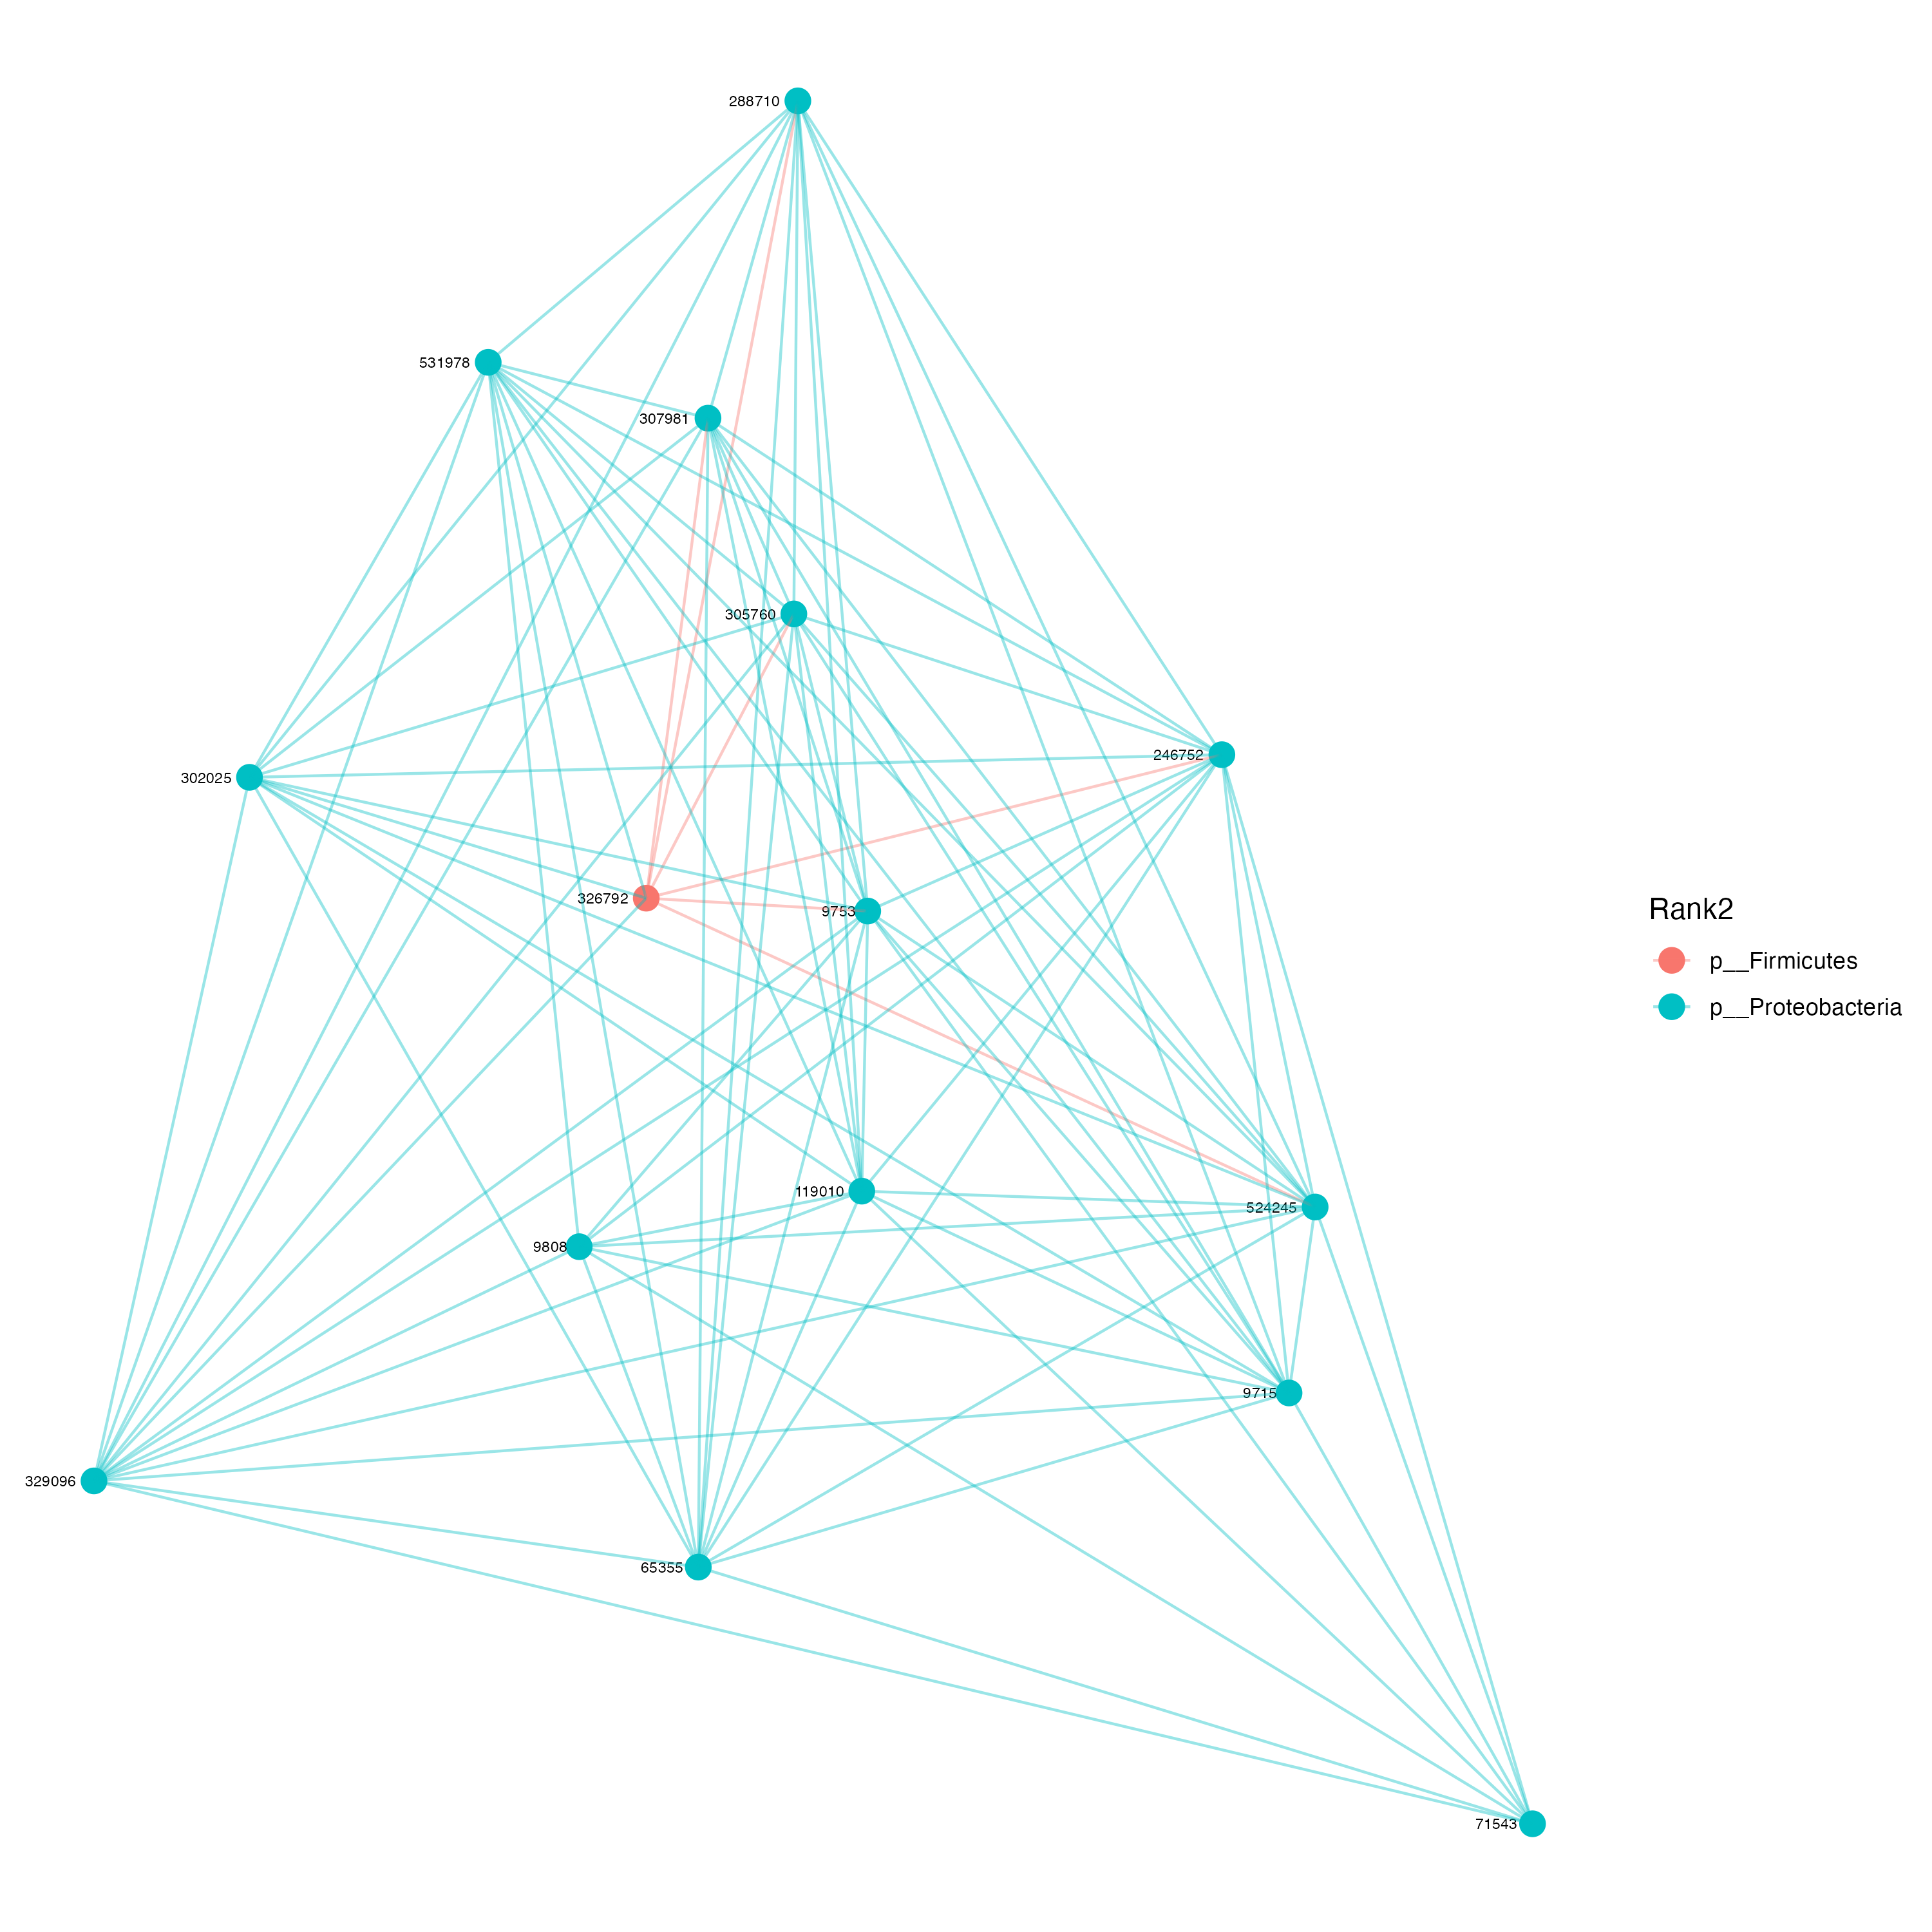
\includegraphics[height=4.7cm]{images/graph-path-gut-15clusters-91edges.png}}
													\subfloat[$2$ clusters]{\label{fig:graph-path-gut-2clusters} 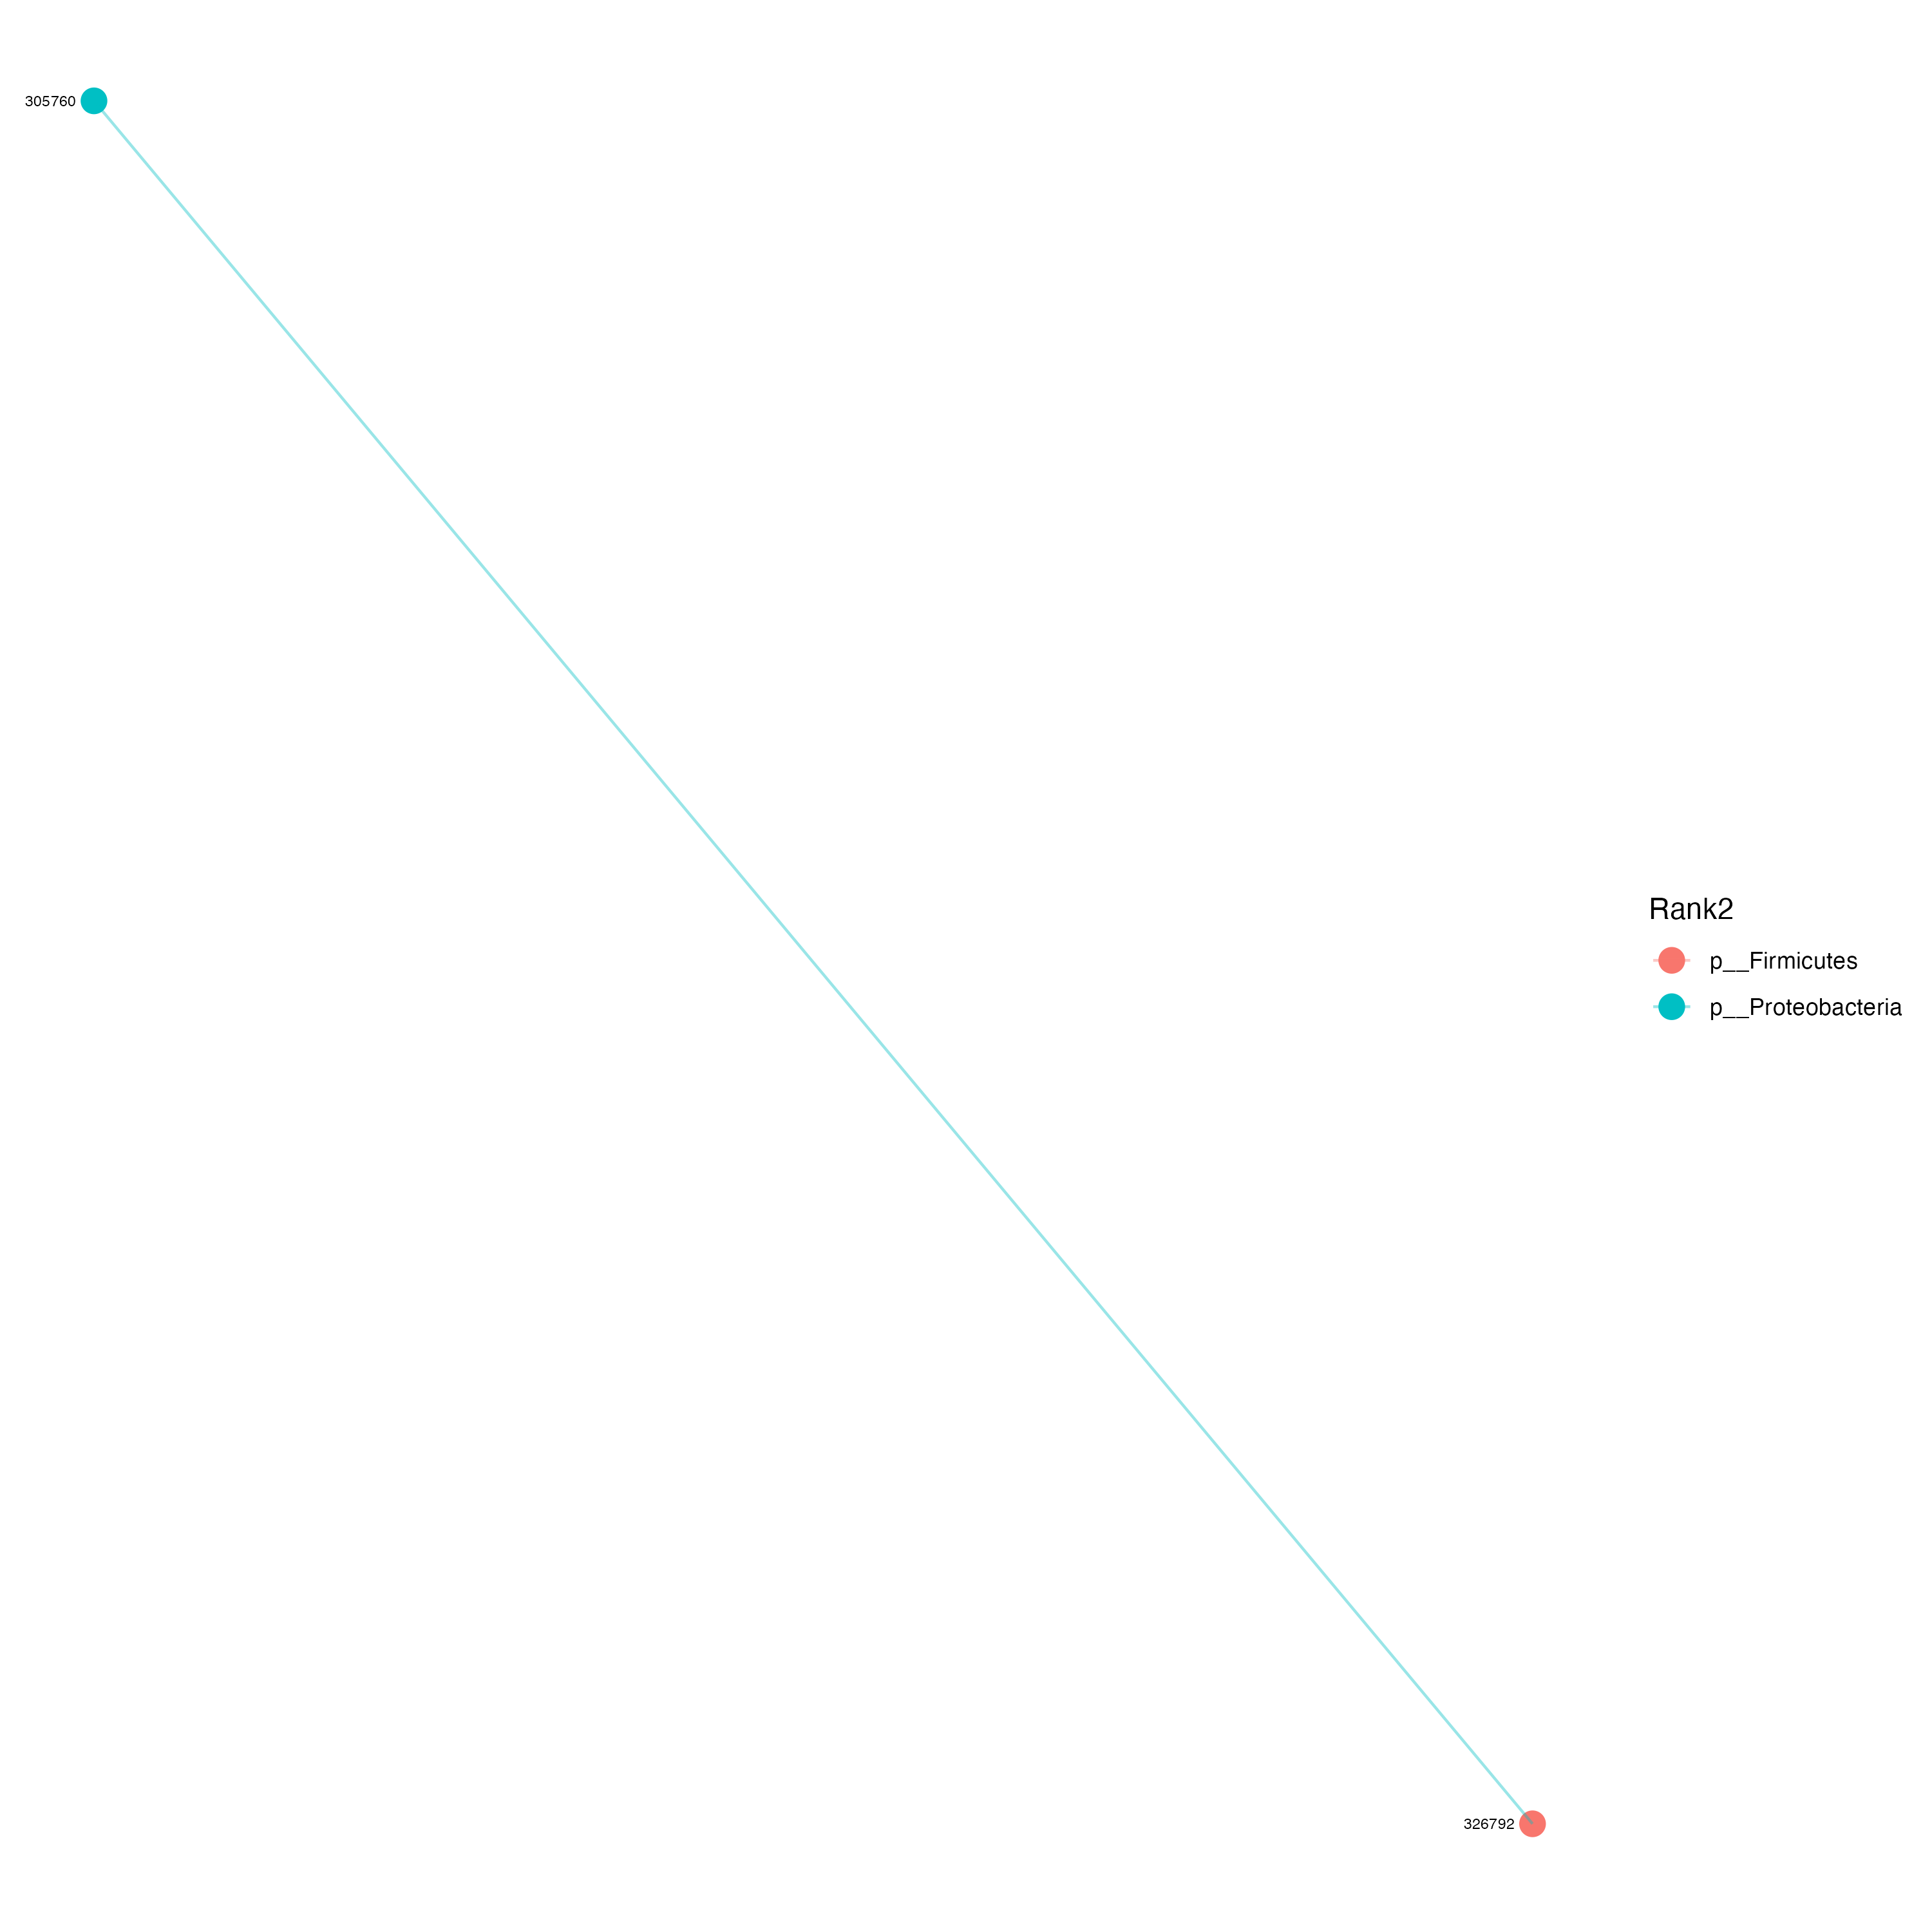
\includegraphics[height=4.7cm]{images/graph-path-gut-2clusters-1edge.png}}
													%\caption{Graphs estimated at multiple levels of granularity for the microbiome data. The first graph, showing a network inferred by the MGLASSO method when $\lambda_2 =0,$ corresponds to the SpiecEasi network. Increasing the fusion penalty makes it possible to uncover graphs built on the representative variable of each cluster. OTUs are colored according to their phylum taxonomic classifier.}
													\label{fig-meta-graphs}
												\end{figure}
											}
										\end{frame}
										

										\section{Simulations}
										\begin{frame}{}
											\begin{center}
												\Huge{\prune{Simulations}}
											\end{center}
											% 	\begin{center}
												% 		\begin{description}
													% 			\item[i] A
													% 			\item[ii] B
													% 			\item[iii] C
													% 		\end{description}
												% 	\end{center}
										\end{frame}
										
										\begin{frame}{}
											Performances evaluated in term of:
											\begin{itemize}
												\item Support recovery: 
												\begin{itemize}
													\item Methods: GLASSO
													\item Simulation model: Stochastic block, Erdos-Renyi and Scale free models
													\item Criterion: ROC curve 
												\end{itemize} 
												\item Clustering: 
												\begin{itemize}
													\item Methods: HAC, $k-$means, Convex clustering, spectral clustering 
													\item Simulation model: Stochastic block and hierarchically structured models 
													\item Criterion: Adjusted Rand Index
												\end{itemize}
											\end{itemize}
										\end{frame}
										
										\subsection{Support recovery}
										\begin{frame}{Graph models}
											\begin{figure}
												\centering
												\begin{subfigure}[b]{0.30\textwidth}
													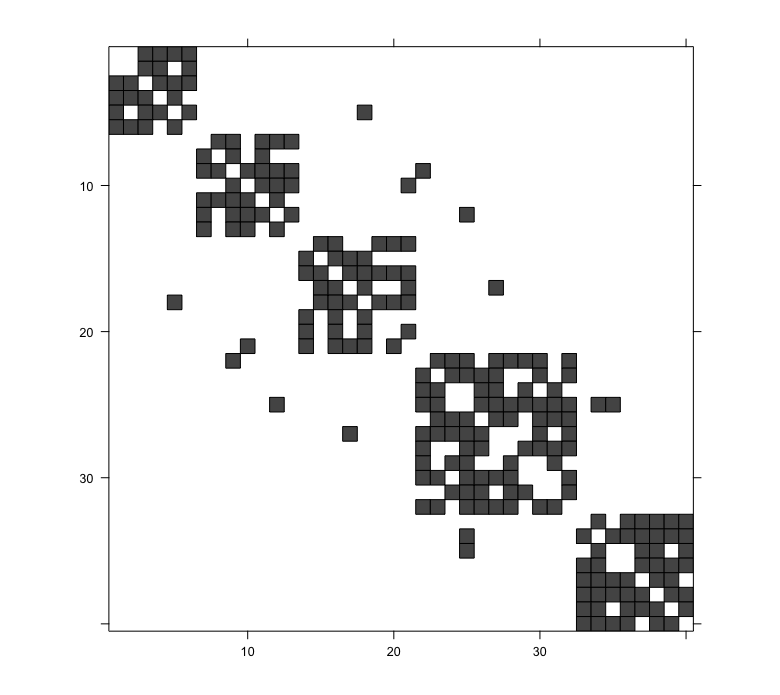
\includegraphics[width=\textwidth]{images/graph_stochastic_block.png}
													\caption{Stochastic block model}
												\end{subfigure}
												\begin{subfigure}[b]{0.30\textwidth}
													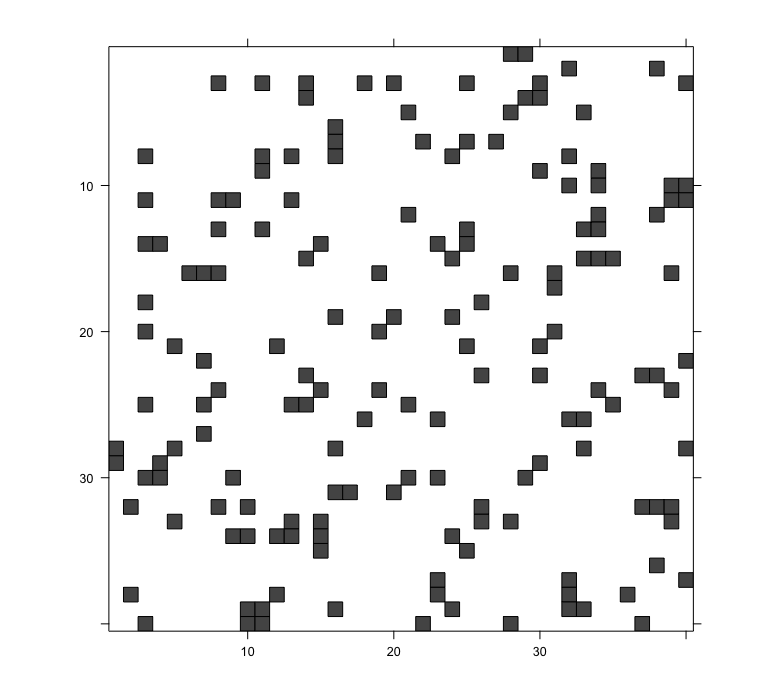
\includegraphics[width=\textwidth]{images/graph_erdos.png}
													\caption{Erdos-Renyi model}
												\end{subfigure}
												\begin{subfigure}[b]{0.30\textwidth}
													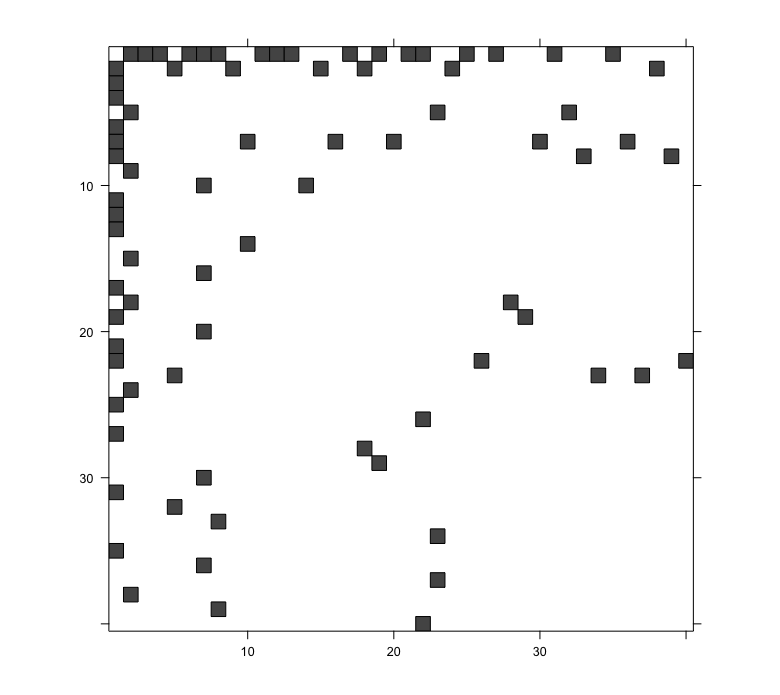
\includegraphics[width=\textwidth]{images/graph_scale_free.png}
													\caption{Scale free model}
												\end{subfigure}
												\caption{Different graph models}
											\end{figure}
										\end{frame}
										
										\begin{frame}{Stochastic block model: settings}
											\begin{figure}
												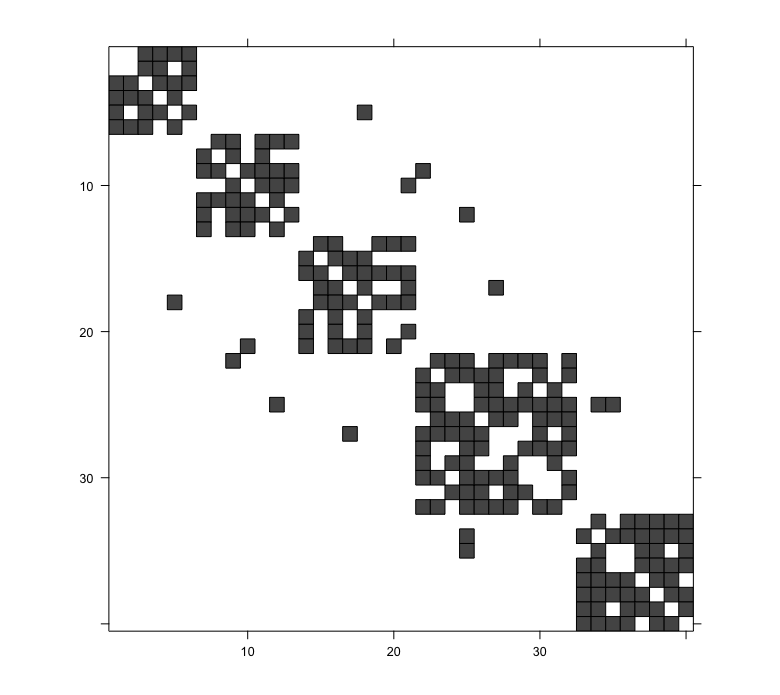
\includegraphics[scale=0.15]{images/graph_stochastic_block.png}
												\caption{Stochastic block model}
											\end{figure}
											Settings
											\begin{itemize}
												\item $p=40$ variables, $\frac{n}{p}\in \{0.5,1,2\}$
												\item $50$ simulations per setting
											\end{itemize}
										\end{frame}
										
										\begin{frame}{Stochastic block model: results}
											\begin{figure}
												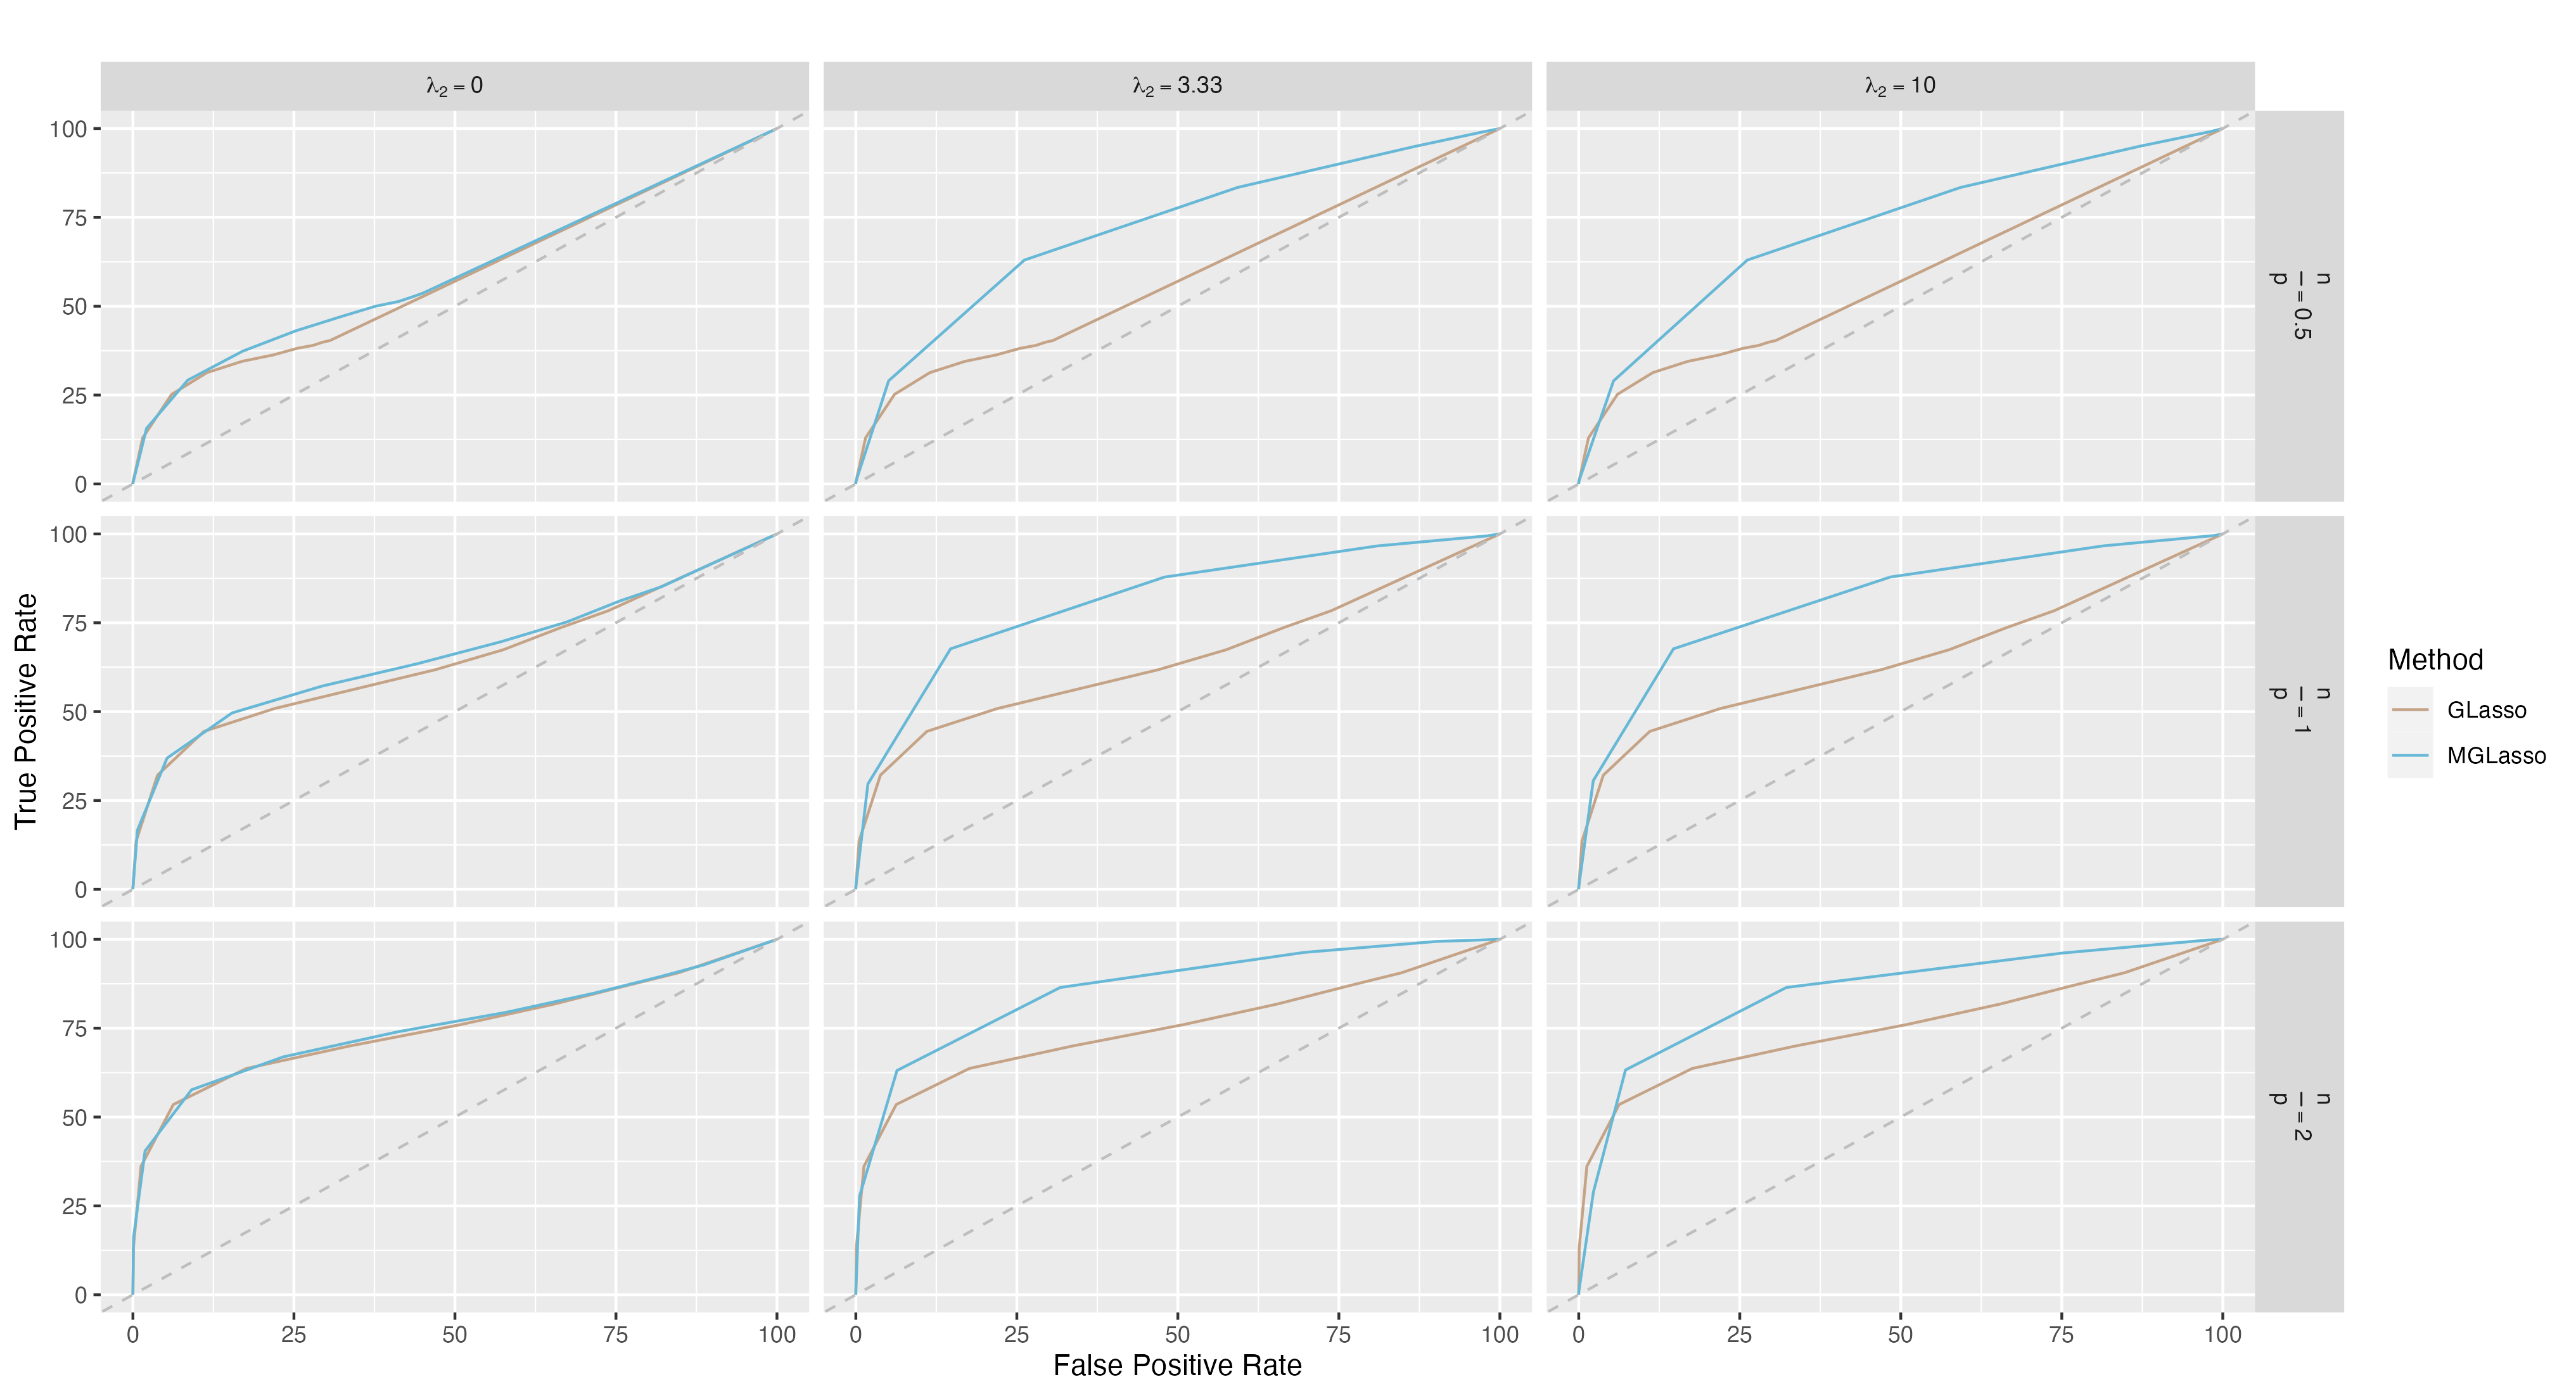
\includegraphics[scale=0.30]{images/fig-roc-sbm.png}
											\end{figure}
										\end{frame}
										

										
										\begin{frame}{Hierarchically structured model}
											\begin{figure}[H]
												\begin{subfigure}[b]{0.4\textwidth}
													\centering
													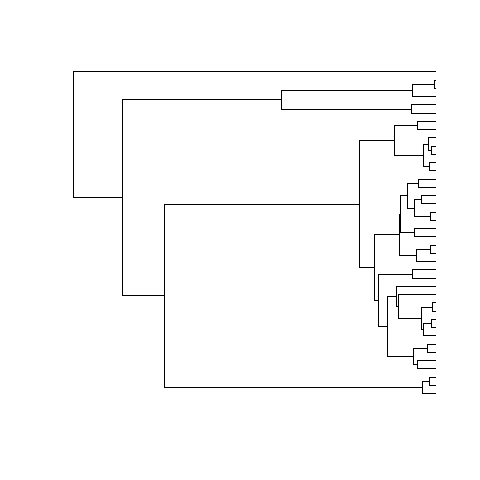
\includegraphics[width=\textwidth]{images/coalescent-tree.png}
													%\caption{Erdös-Rényi model}
													%\label{fig:parameter-tuning-erdos}
												\end{subfigure}
												\hfill
												\begin{subfigure}[b]{0.4\textwidth}
													\centering
													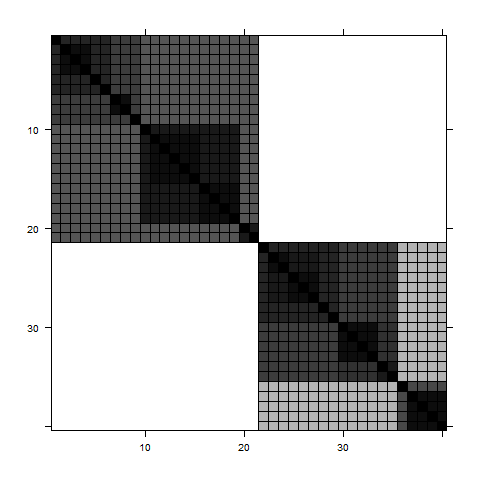
\includegraphics[width=\textwidth]{images/cov-mat-OU-process-on-coalescent-tree.png}
													%\caption{scale-free model}
													%\label{fig:parameter-tuning-sfree}
												\end{subfigure}
												% 		\hfill
												% 		\begin{subfigure}[b]{0.3\textwidth}
													% 			\centering
													% 			\includegraphics[width=4.5cm]{images/prec-mat-OU-process-on-coalescent-tree.png}
													% 			%\caption{Stochastic block model}
													% 			%\label{fig:parameter-tuning-sbm}
													% 		\end{subfigure}
												\caption{Tree, Covariance matrix of the phylogeny based hierarchical model}
												\label{fig:hierarchical-model}
											\end{figure}
										\end{frame}
										
										\begin{frame}{Hierarchically structured model: results}
											\begin{figure}
												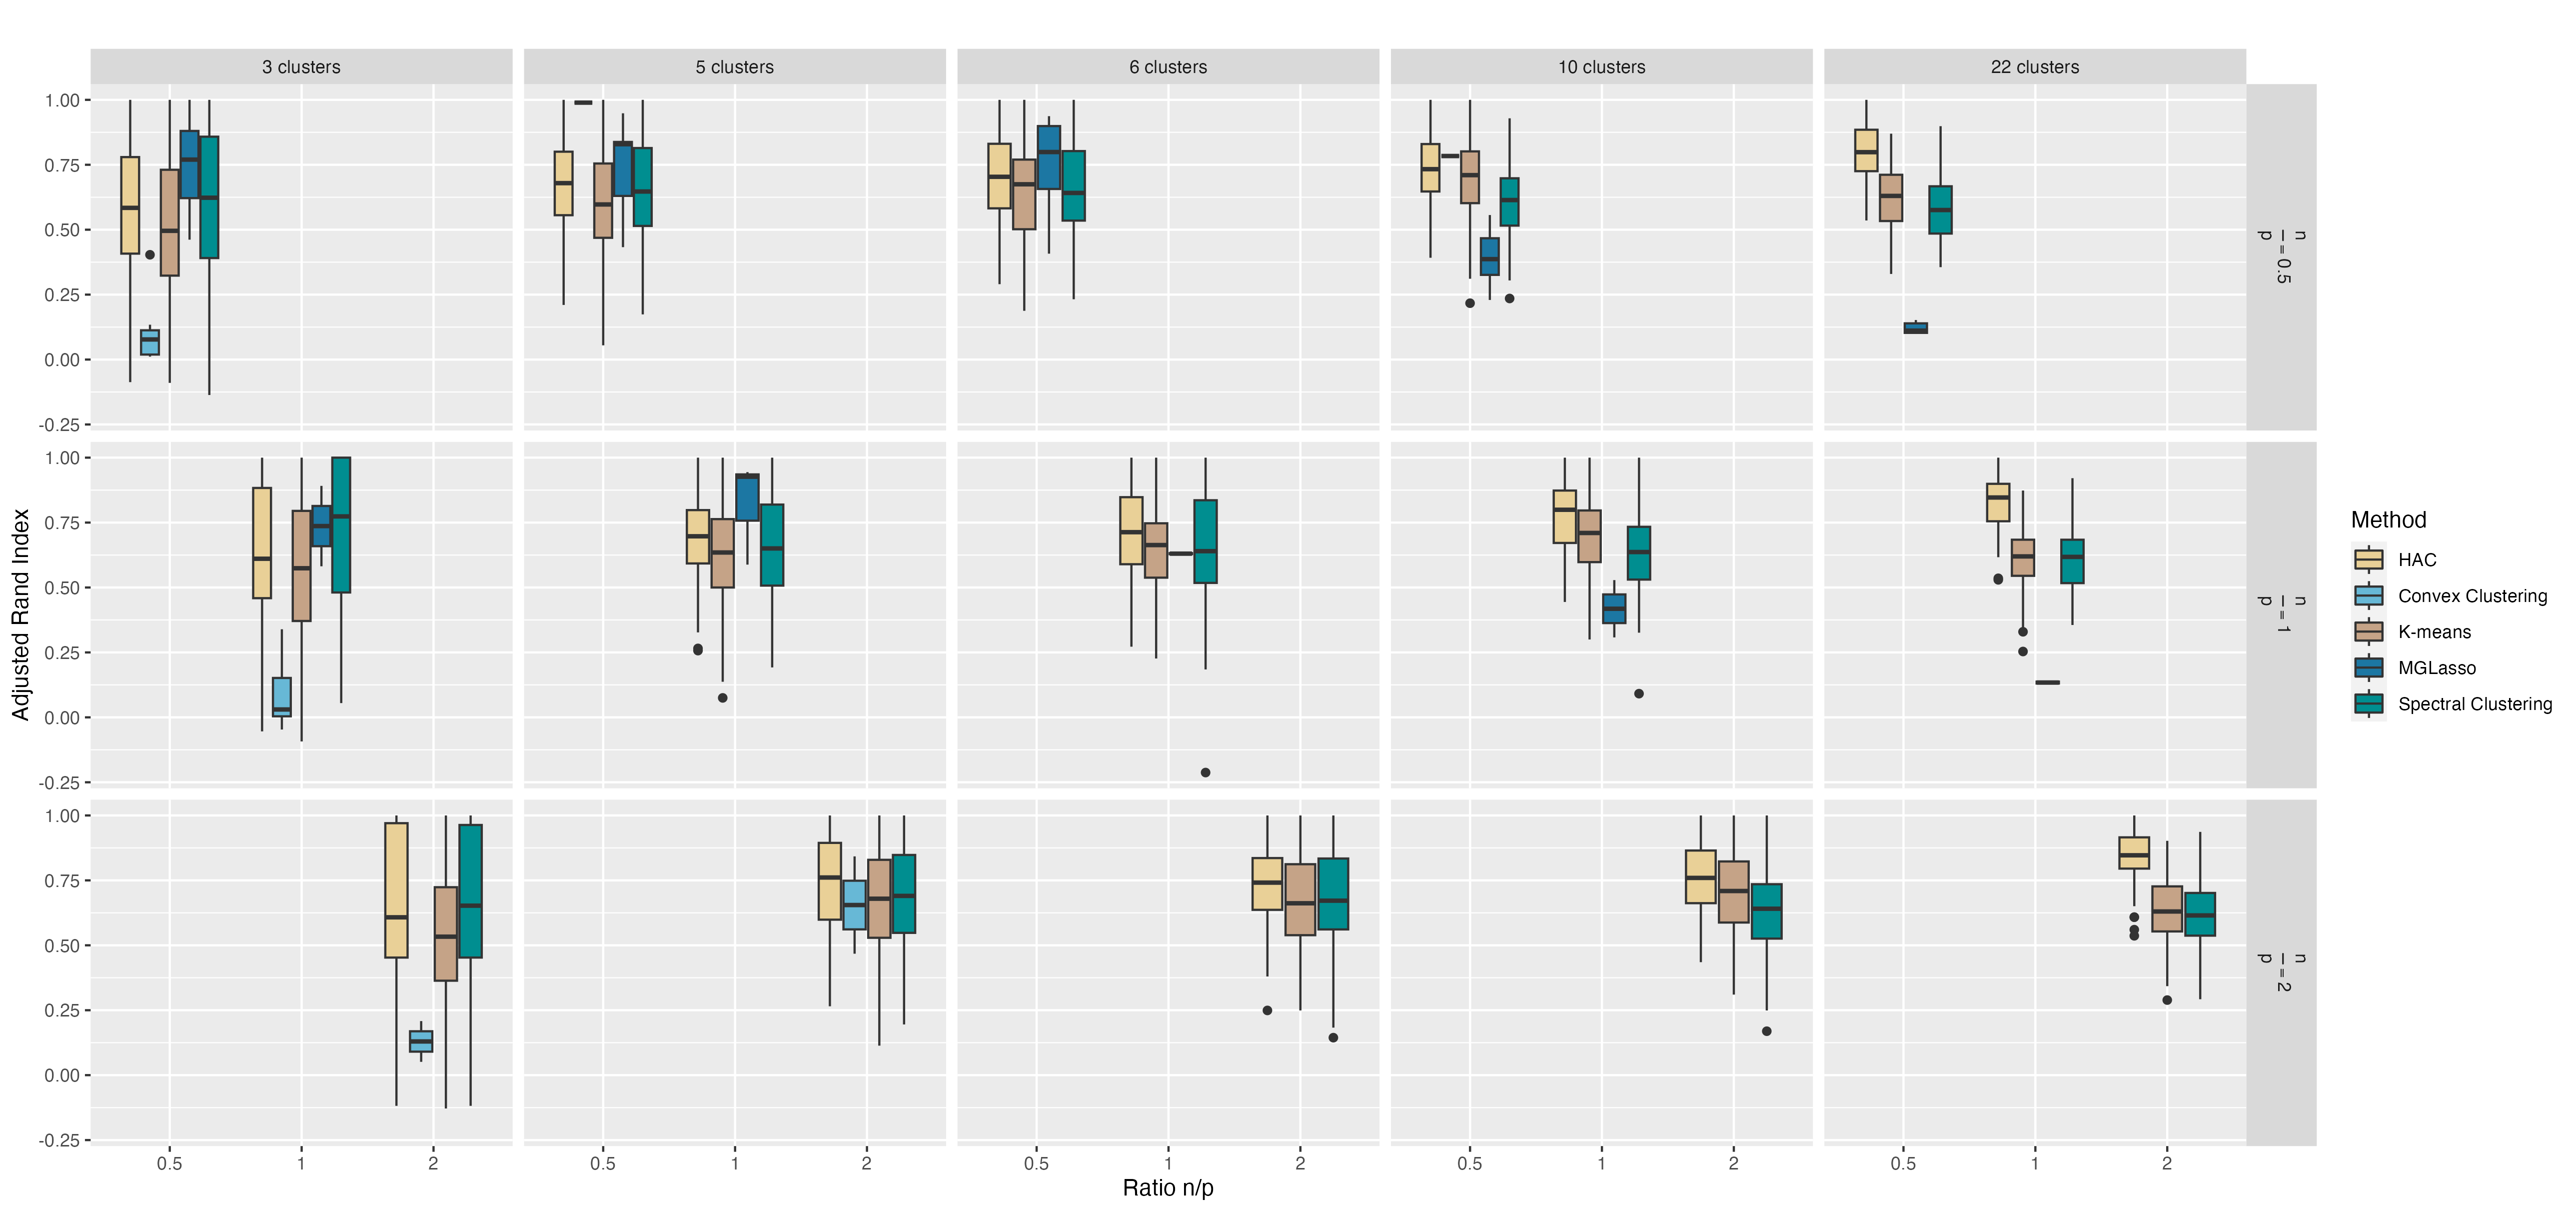
\includegraphics[scale=0.28]{images/tree-model-perf-rand.png}
											\end{figure}
										\end{frame}
										
										
										\section{Miscellaneous}
										\subsection{Convex clustering}
										
										
										\begin{frame}{Graphical models + Convex clustering: Relevant Works}
											\begin{itemize}
												\item \textcolor{Framaprune}{Clustered Gaussian Graphical Model Via Symmetric Convex Clustering \citep{Yao2019}}:
												\begin{equation}
													\min_{\Theta, \{\Psi_l\}} -\log \det \Omega + \tr{\hat \Sigma \Omega} + \lambda \sum_{l \in \mathcal M}^{} w_l \normldeux{\Psi_{l,1} - \Psi_{l,2}} 
												\end{equation}
												subject to $(Q_l \Theta R_l) - \Psi_l = 0, \forall l \in \mathcal M.$
												
												\item \textcolor{Framaprune}{Estimation of Sparse Gaussian Graphical Models with Hidden Clustering Structure \citep{lin2020estimation}}:
												\begin{equation} 
													\operatorname{max}_{\bO \in \mathbb S_{\succ 0 }^p} \left \{ \log \det (\bO) - \tr(\bS \bO) - \lambda_1 \sum_{i<j} |\bO_{ij}| - \lambda_2 \sum_{i <j} \sum_{s < t} | \bO_{ij} - \bO_{st} | \right \}
												\end{equation}
											\end{itemize}
										\end{frame}
										
										\begin{frame}{Convex Clustering with Weights}
											\begin{equation}
												\label{eq:convex-clust}
												\frac{1}{2} \sum_{i=1}^n \normldeux{x_i - \alpha_i}^2 + \lambda \sum_{i < j} w_{ij} \normlq{\alpha_i - \alpha_j}
											\end{equation}
											
											\textcolor{Framaprune}{Distance Decreasing Weights}:
											\begin{itemize}
												\item Empirical approach \cite{Hocking2011, chi2019recovering}: $w_{ij} = \exp \left (-\gamma \normldeux{x_i - x_j}^2 \right)$ (Gaussian kernel)
												\item Theoretical approach \cite{chiquet2017fast}: $w_{ij} = f \left(\normlq{x_i - x_j} \right)$ ($\ell_1$ case, and multimensional clusterpath problem).
												\begin{equation}
													\sum_{i=1}^{p} \left[ \frac{1}{2} \sum_{i=1}^n (x_{ik} - \alpha_{ik})^2  + \lambda \sum_{i < j} w_{ij} \abs{\alpha_{ik} - \alpha_{jk}}\right] 
												\end{equation}
											\end{itemize}
										\end{frame}
										
										\begin{frame}{Conditional Gaussian Distribution}
											Given $\bX^{\backslash j} = \bm Z$, the conditional distribution of $\bX^j = Y$ is Gaussian.
											
											Partitioning $\bm \Sigma$:
											$$\bm \Sigma = \begin{pmatrix}
												\Sigma_{YY} & \Sigma_{YZ}\\
												\Sigma_{ZY} & \bm \Sigma_{ZZ}
											\end{pmatrix}$$
											
											The conditional distribution:
											$$Y|\bm Z=z \sim \mathcal N\left((z-\mu_Z)^T \bm \Sigma_{ZZ}^{-1} \Sigma_{ZY}, \Sigma_{YY} - \Sigma_{ZY}^T \bm \Sigma_{ZZ}^{-1} \Sigma_{ZY}\right)$$
											
											Using Schur complement and partitioning $\bm \Omega$:
											$$Y|\bm Z=z \sim \mathcal N\left((z-\mu_Z)^T (-\bm \Omega_{YZ}/\Omega_{YY}), \Omega_{YY}^{-1}\right)$$
											
											Log-likelihood of univariate-conditional normal distribution:
											\begin{equation*}
												\begin{split}
													\log p(Y|\bm Z) &= \frac{1}{2} \text{log}(\Omega_{YY}) - \frac{1}{2} \Omega_{YY} \left (y + \frac{\bm \Omega_{YZ}}{\Omega_{YY}} z \right )^2 + \text{const}
												\end{split}
											\end{equation*}
										\end{frame}
										
									\backupend
									\end{document}